\clearpage
\section{Data availability statement}

The \href{https://github.com/Photonico/H-Beryllene_20250718}{beryllene repository on GitHub} contains the calculation data for this chapter.

\FloatBarrier
\section{Supplementary information}
\label{3_supplementary}

We first check the convergence of the cohesive and total energies with the k-point mesh.
Figures~\ref{fig:proj3_cohesive_energy_convergence} and~\ref{fig:proj3_total_energy_convergence}
show these tests.

We also test the sensitivity of the cohesive energies to dispersion by adding the D3 energy with Becke--Johnson damping at the PBE geometries.
The cohesive energies of $\alpha$-beryllene, $\beta$-beryllene, and trilayer cubic beryllene then lie \qty{1.04}{\electronvolt}, \qty{0.60}{\electronvolt}, and \qty{0.56}{\electronvolt} per atom above that of bulk hcp beryllium.
Without the correction, these differences are \qty{0.79}{\electronvolt}, \qty{0.44}{\electronvolt}, and \qty{0.43}{\electronvolt} per atom.
The correction therefore favours bulk hcp beryllium relative to these three layers and preserves their energy ordering.

\begin{figure}[!htbp]
\centering
\begin{tabular}{@{}cc@{}}
    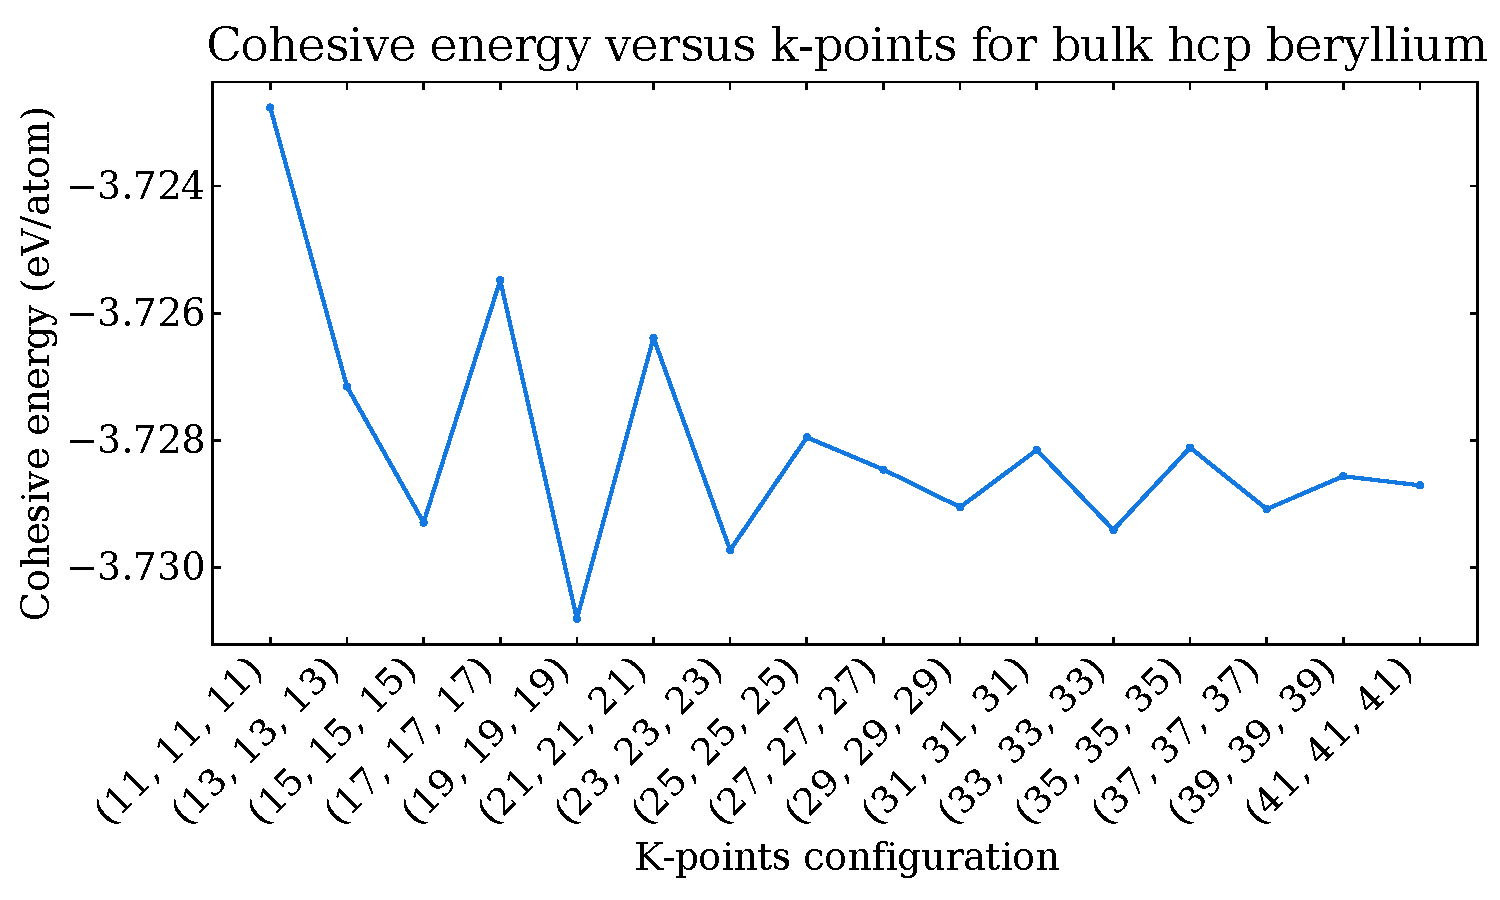
\includegraphics[width=0.40\linewidth]{figures_proj3/convergence_cohesive_kpoints_hcp-beryllium_thesis.pdf}&
    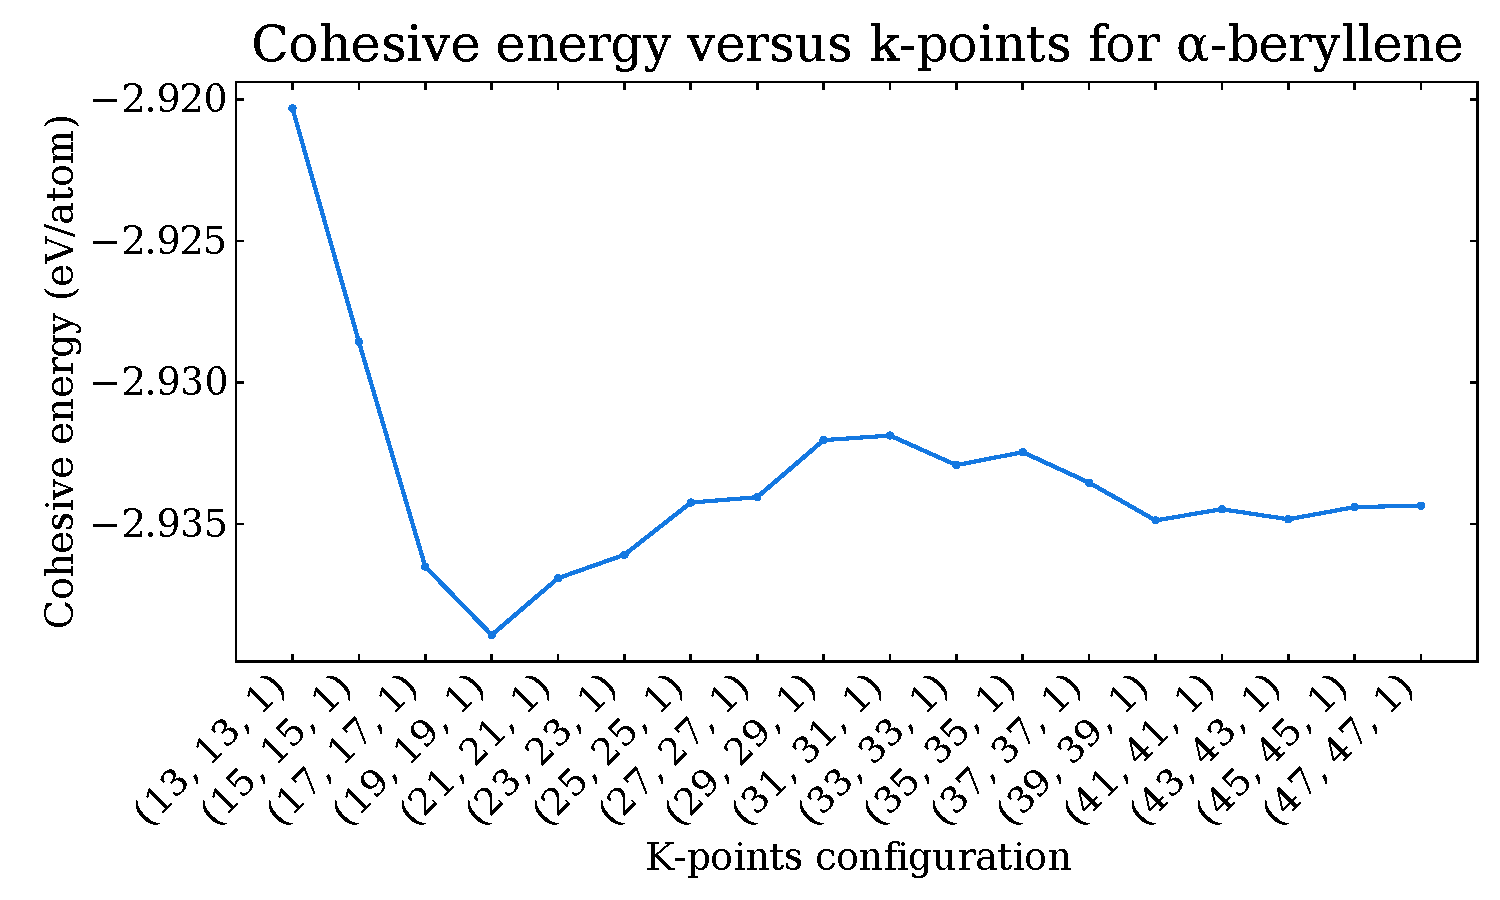
\includegraphics[width=0.40\linewidth]{figures_proj3/convergence_cohesive_kpoints_alpha-beryllene_thesis.pdf}\\
    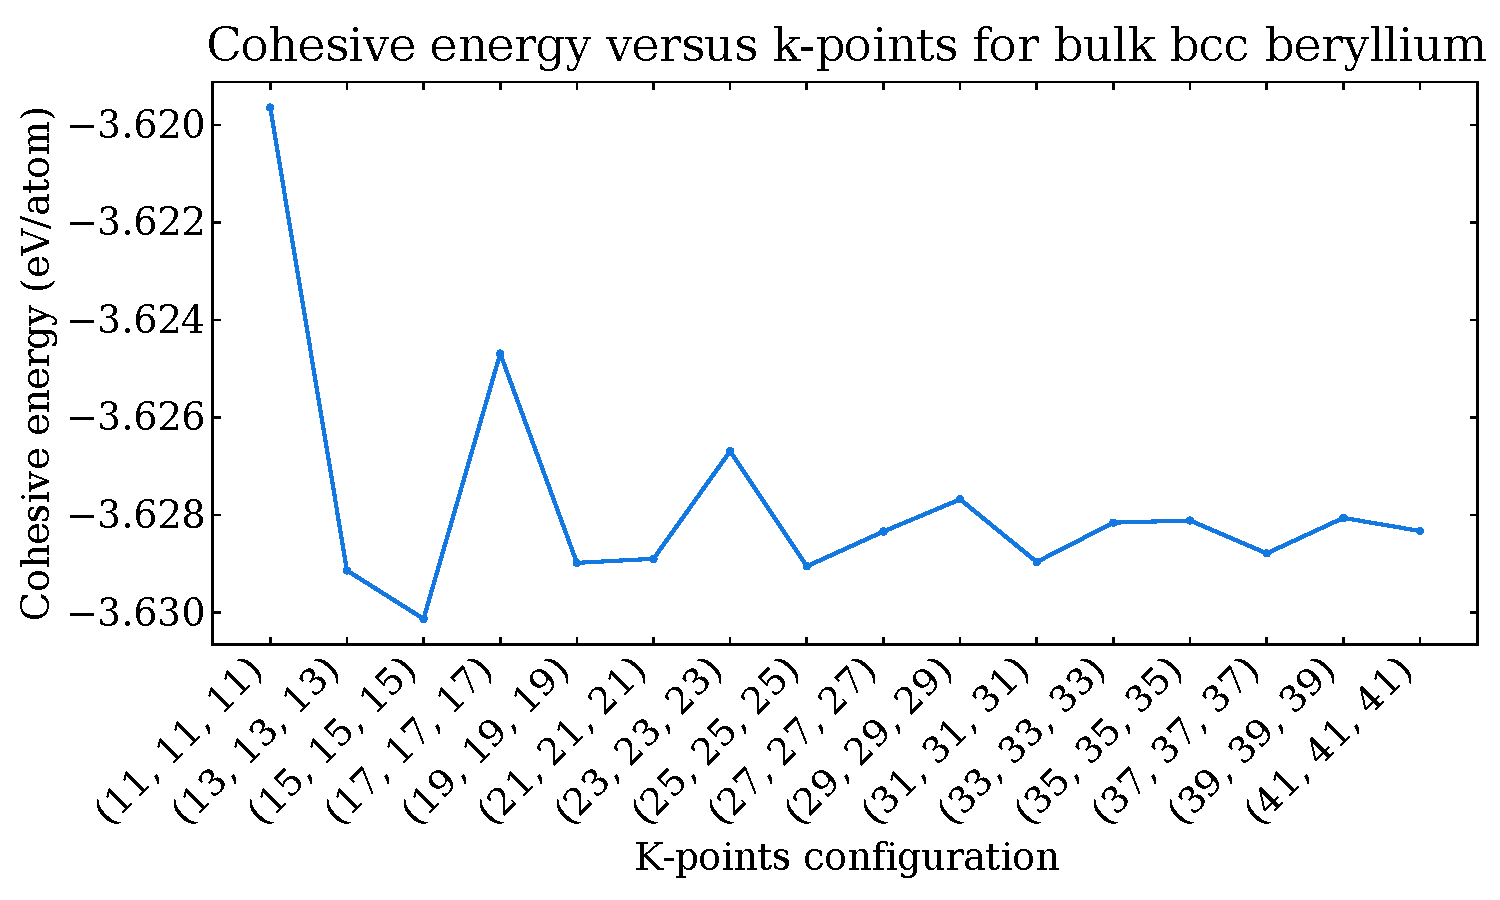
\includegraphics[width=0.40\linewidth]{figures_proj3/convergence_cohesive_kpoints_bcc-beryllium_thesis.pdf}&
    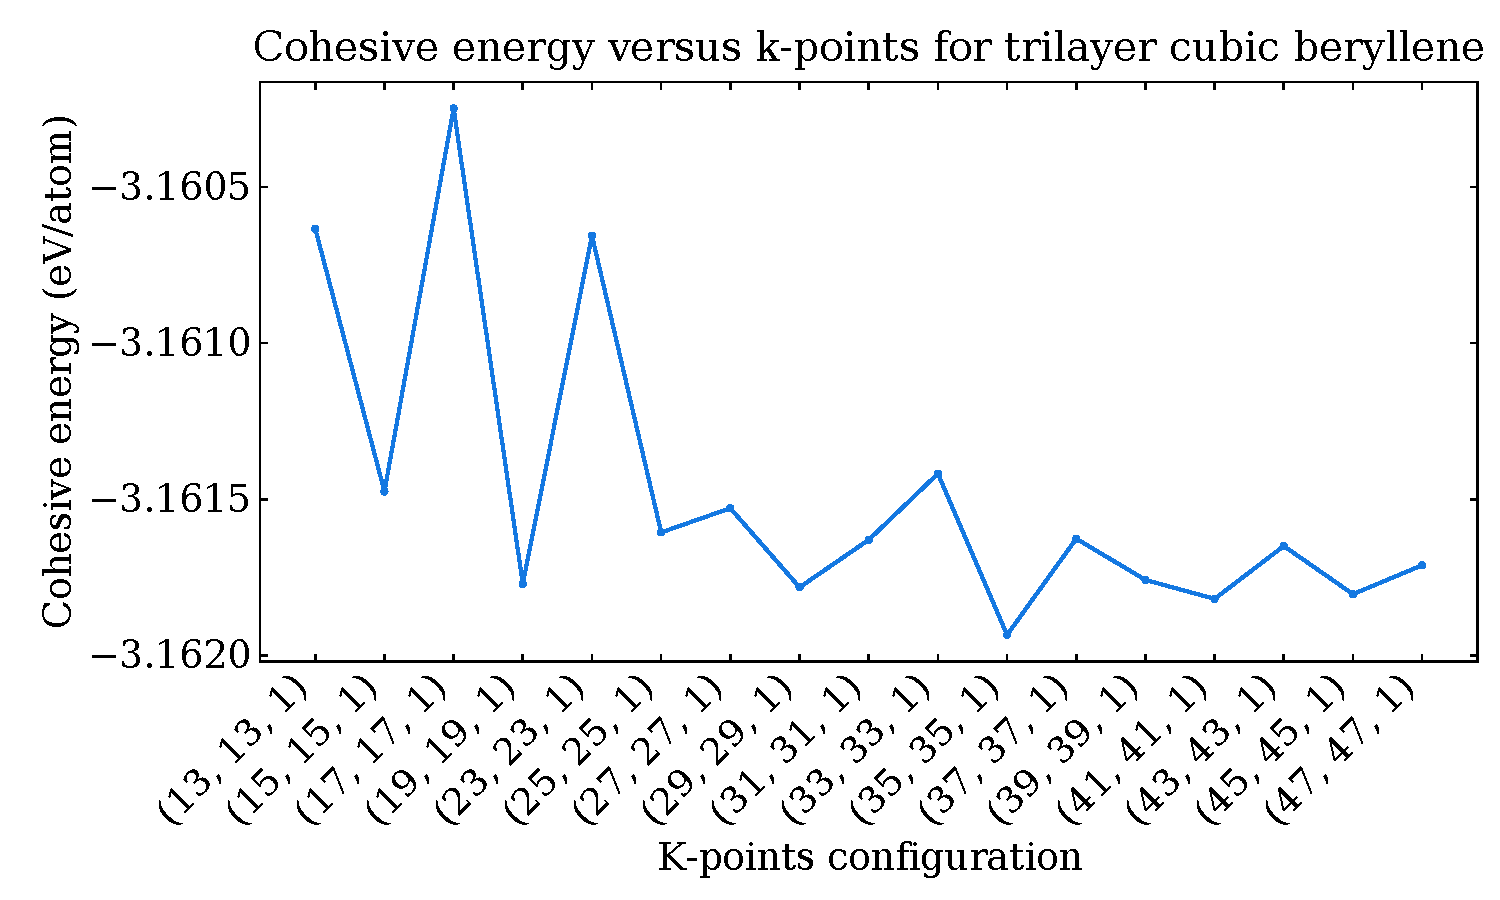
\includegraphics[width=0.40\linewidth]{figures_proj3/convergence_cohesive_kpoints_cubic-beryllene-trilayer_thesis.pdf}
\end{tabular}
\caption{Cohesive energy as a function of the k-point mesh for bulk hcp beryllium, $\alpha$-beryllene, bulk bcc beryllium, and trilayer cubic beryllene.}
\label{fig:proj3_cohesive_energy_convergence}
\end{figure}

\begin{figure}[!htbp]
\centering
\begin{tabular}{@{}cc@{}}
    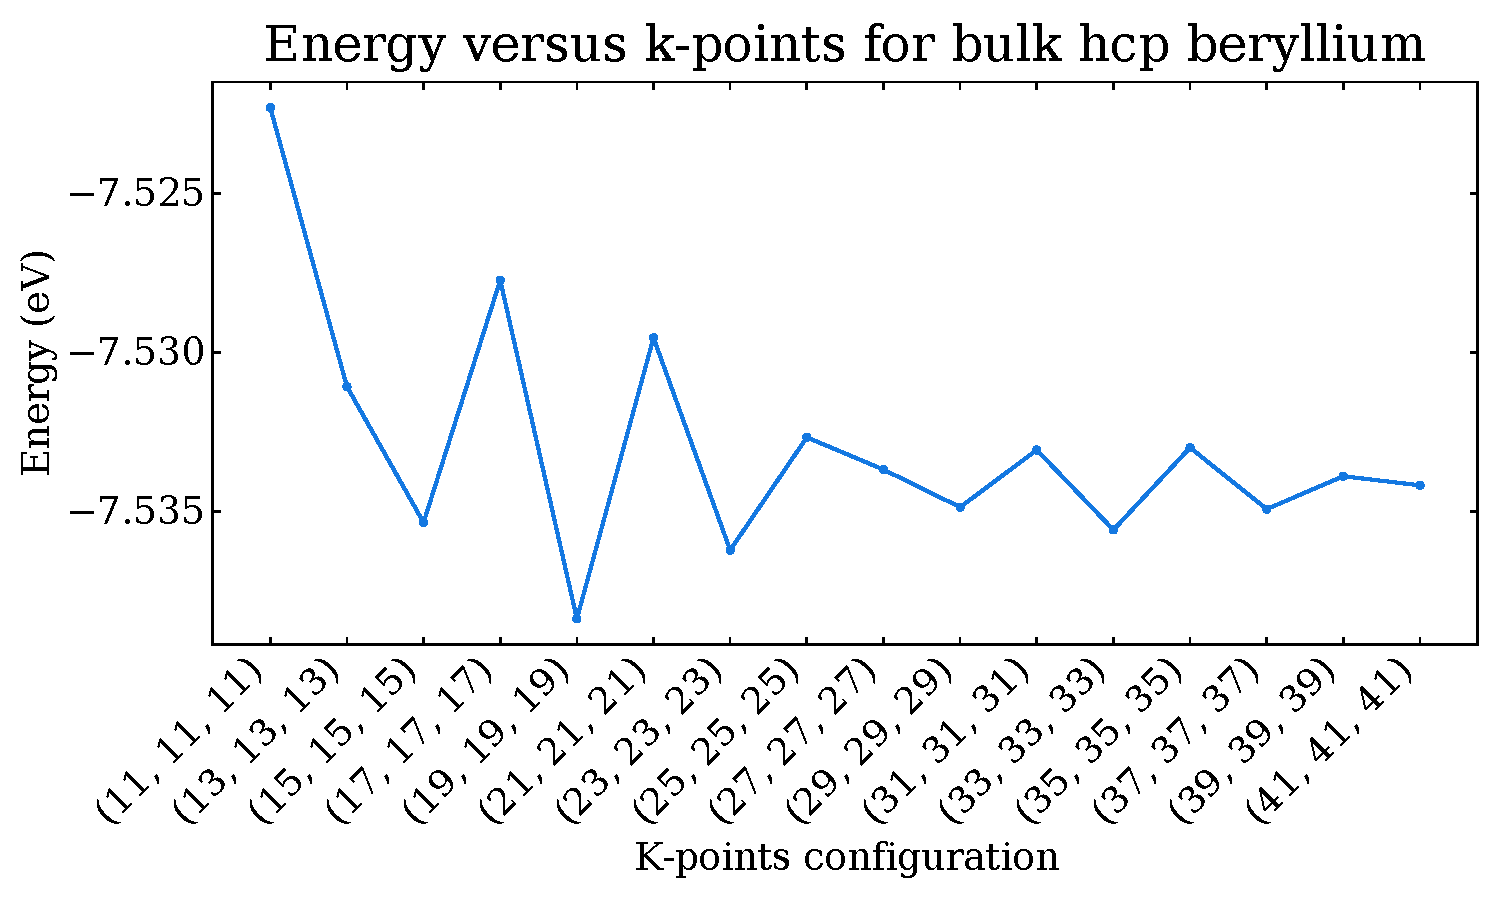
\includegraphics[width=0.40\linewidth]{figures_proj3/convergence_energy_kpoints_hcp-beryllium_thesis.pdf}&
    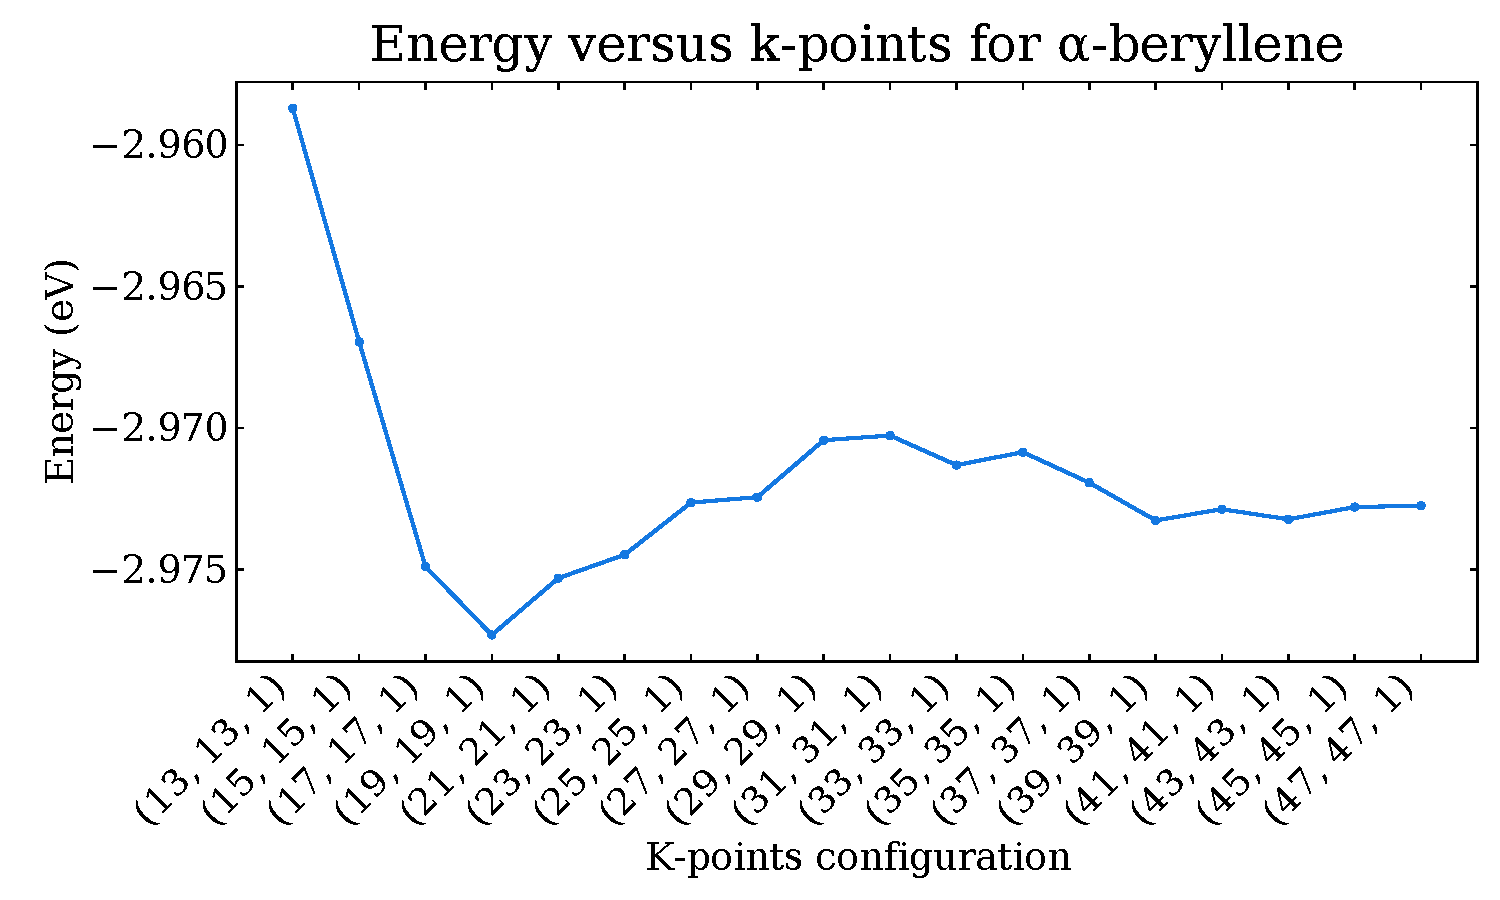
\includegraphics[width=0.40\linewidth]{figures_proj3/convergence_energy_kpoints_alpha-beryllene_thesis.pdf}\\
    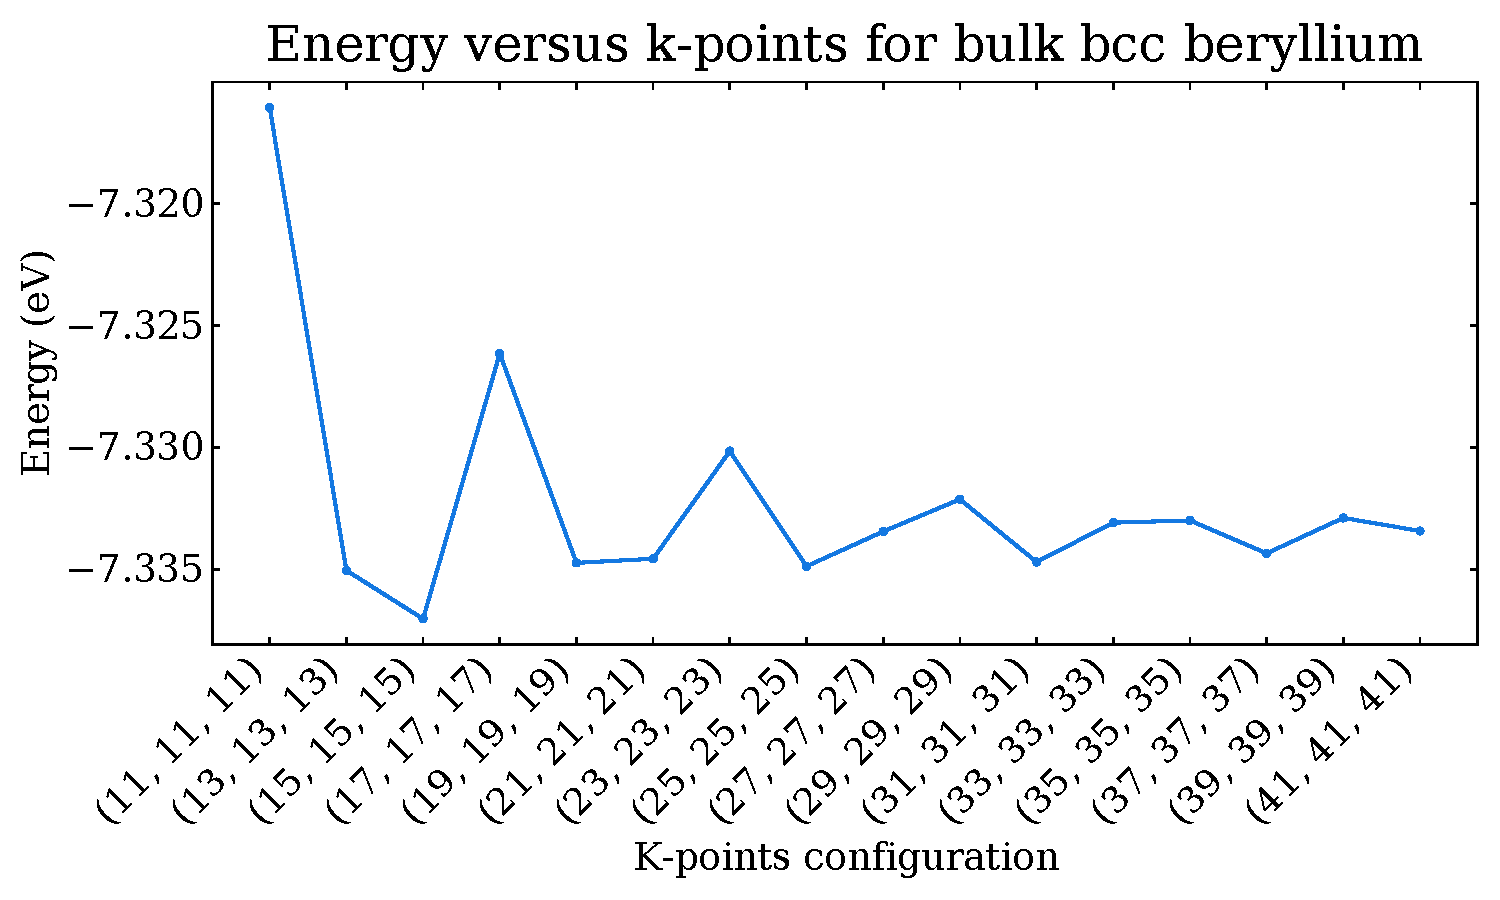
\includegraphics[width=0.40\linewidth]{figures_proj3/convergence_energy_kpoints_bcc-beryllium_thesis.pdf}&
    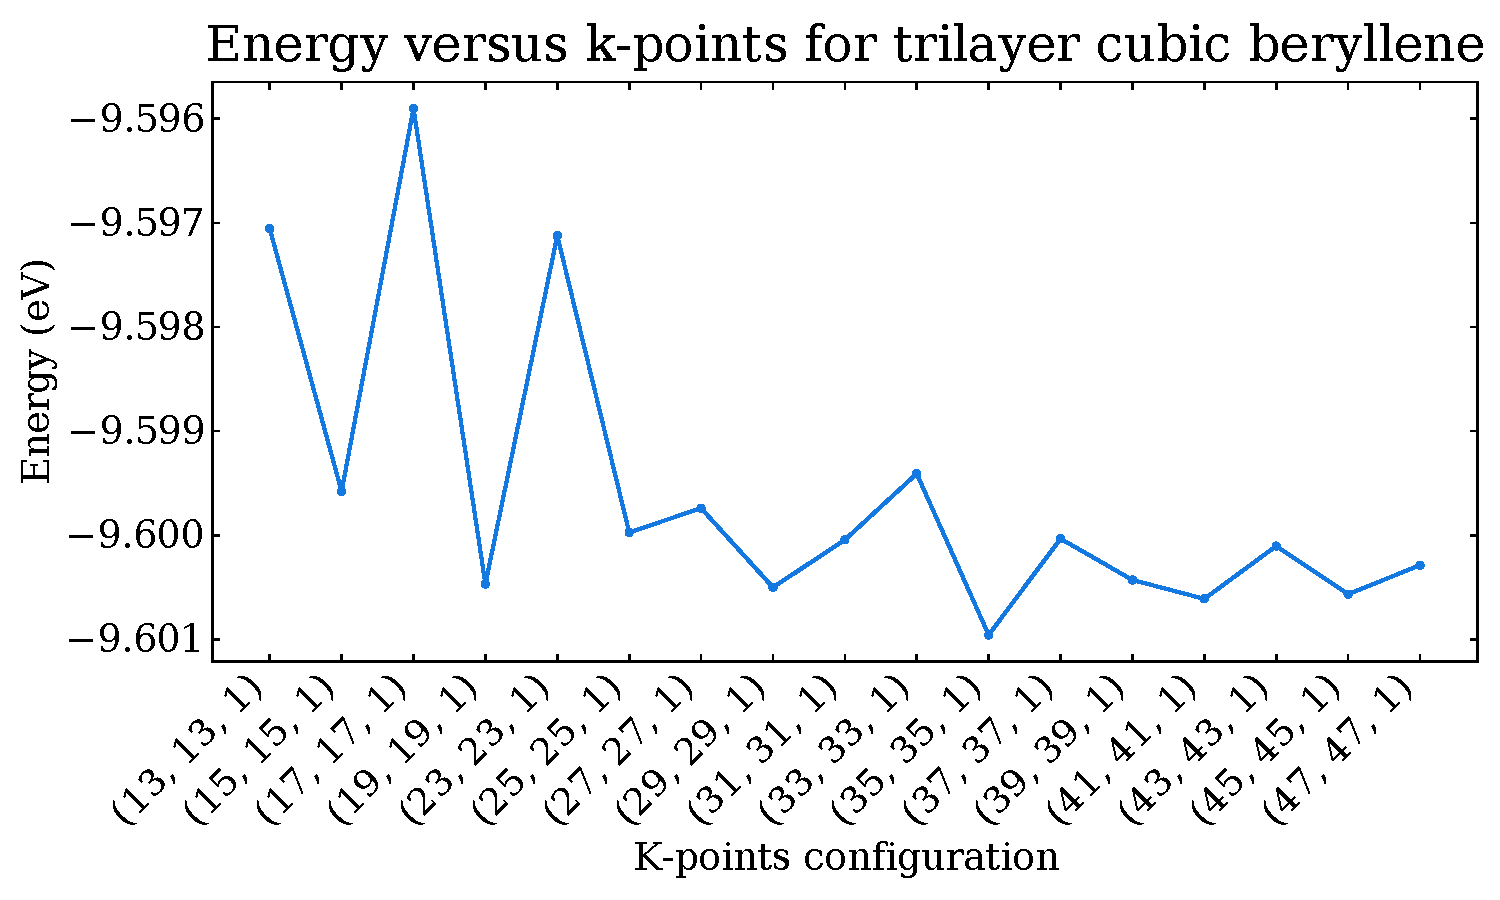
\includegraphics[width=0.40\linewidth]{figures_proj3/convergence_energy_kpoints_cubic-beryllene-trilayer_thesis.pdf}
\end{tabular}
\caption{Total energy as a function of the k-point mesh for bulk hcp beryllium, $\alpha$-beryllene, bulk bcc beryllium, and trilayer cubic beryllene.}
\label{fig:proj3_total_energy_convergence}
\end{figure}

\FloatBarrier
\subsection*{Optical-calculation parameters}

We use the optical definitions in section~\ref{sec:from_dielectric_function_to_optical_properties}
and the volume normalization in equation~\eqref{optical_volume_normalization_2d}.
The effective thicknesses $d_{\mathrm{2D}}$ in this normalization are
\qty{3.960}{\angstrom} for pristine $\alpha$-beryllene,
\qty{5.869}{\angstrom} for pristine $\beta$-beryllene,
\qty{6.966}{\angstrom} for trilayer cubic beryllene,
\qty{3.145}{\angstrom} for 2H-$\alpha$-beryllene,
\qty{5.524}{\angstrom} for 1H-$\beta$-beryllene,
and \qty{5.193}{\angstrom} for 2H-$\beta$-beryllene.
We remove periodic wrapping before measuring the separation of the outermost atomic centres along the surface normal.
The radius correction uses two Be radii for pristine layers, two H radii for double-sided termination, and one of each for single-sided termination.
The smaller H radius makes the assigned thickness of 2H-$\alpha$-beryllene shorter than that of pristine $\alpha$-beryllene under this convention.
We use the unrounded thicknesses in all calculations.

The calculations use 140 bands for each hydrogen-functionalized structure,
133 for pristine $\alpha$-beryllene and trilayer cubic beryllene,
128 for pristine $\beta$-beryllene,
70 for bulk bcc beryllium,
and 66 for bulk hcp beryllium.
These numbers include both occupied and unoccupied bands.
The total can differ from the requested \texttt{NBANDS} because the code allocates bands in groups for parallel execution.

\FloatBarrier
\subsection*{Dielectric-function convergence}

We test the interband dielectric response against the total band count and the k-point mesh.
Figures~\ref{fig:proj3_hcp_dielectric_nbands_convergence}--\ref{fig:proj3_cubic_dielectric_kpoint_convergence}
show the tests for bulk hcp beryllium, $\alpha$-beryllene, $\beta$-beryllene, bulk bcc beryllium, and trilayer cubic beryllene.
The reference curves use the final settings, whose meshes and band counts can differ from those in the convergence series.
The plots retain the full height of each curve in the displayed energy window.
In particular, figure~\ref{fig:proj3_hcp_dielectric_kpoint_convergence} shows a large low-energy response for the $45 \times 45 \times 45$ mesh of bulk hcp beryllium.

\begin{figure}[!htbp]
\centering
    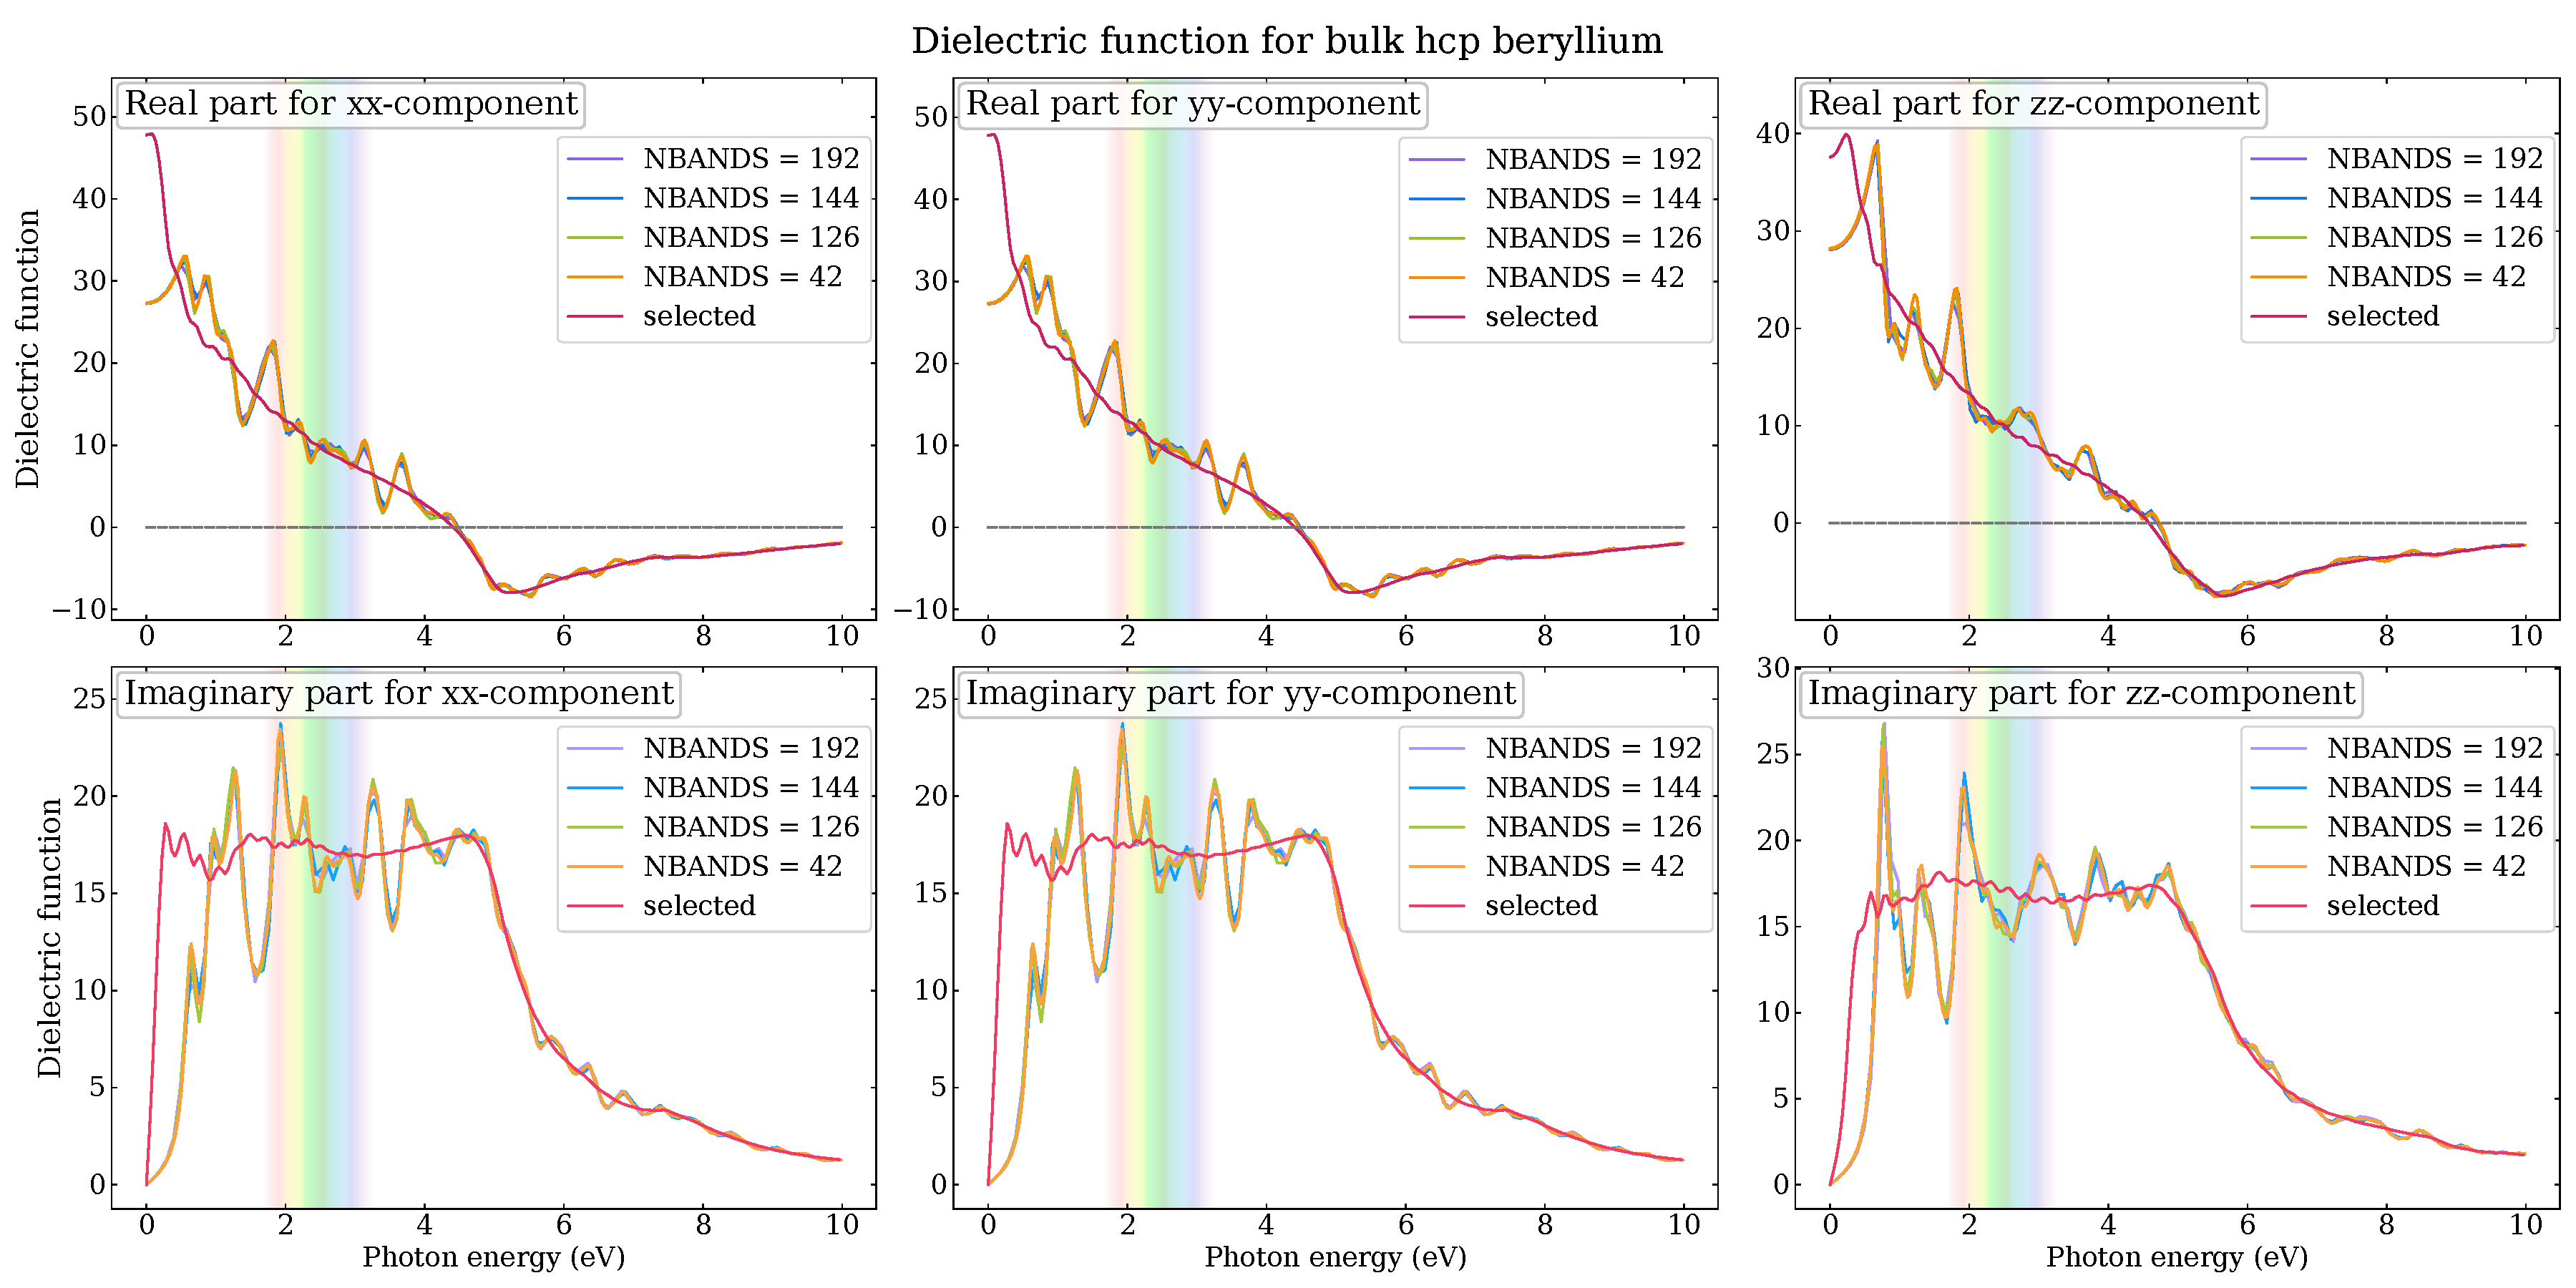
\includegraphics[width=1.0\linewidth]{figures_proj3/convergence_dielectric_nbands_hcp-beryllium_thesis.pdf}
\caption{Real and imaginary parts of the dielectric function for bulk hcp beryllium,
calculated with different total numbers of bands.}
\label{fig:proj3_hcp_dielectric_nbands_convergence}
\end{figure}

\begin{figure}[!htbp]
\centering
    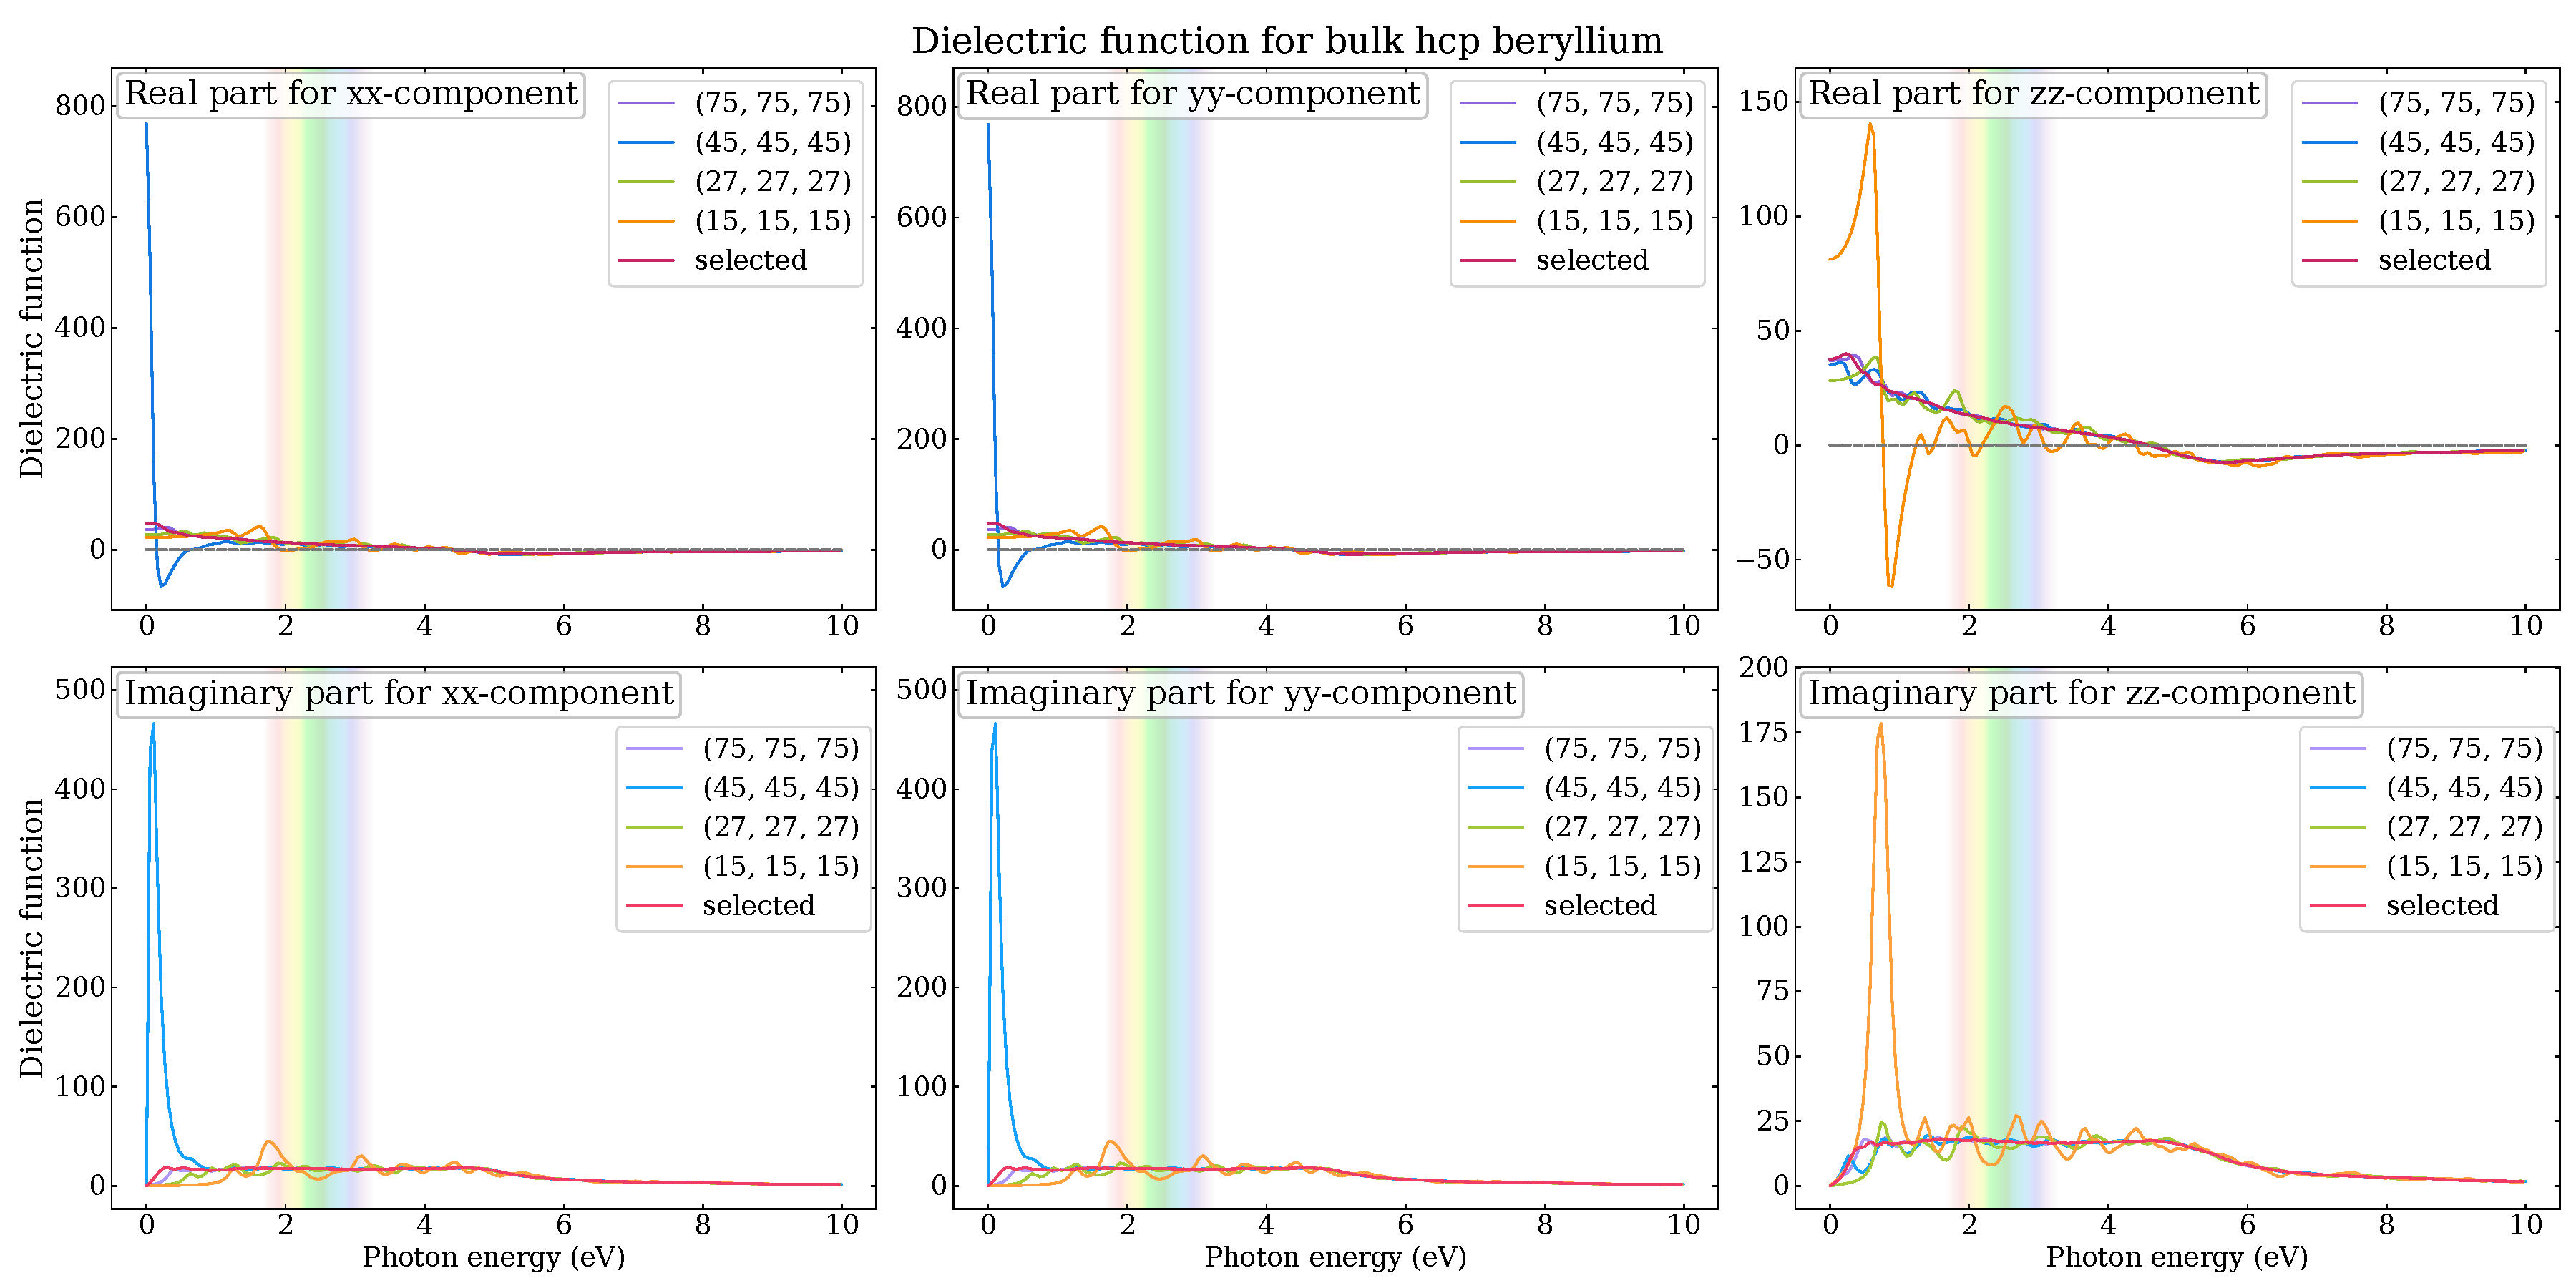
\includegraphics[width=1.0\linewidth]{figures_proj3/convergence_dielectric_kpoints_hcp-beryllium_thesis.pdf}
\caption{Real and imaginary parts of the dielectric function for bulk hcp beryllium,
calculated with different k-point meshes.}
\label{fig:proj3_hcp_dielectric_kpoint_convergence}
\end{figure}

\begin{figure}[!htbp]
\centering
    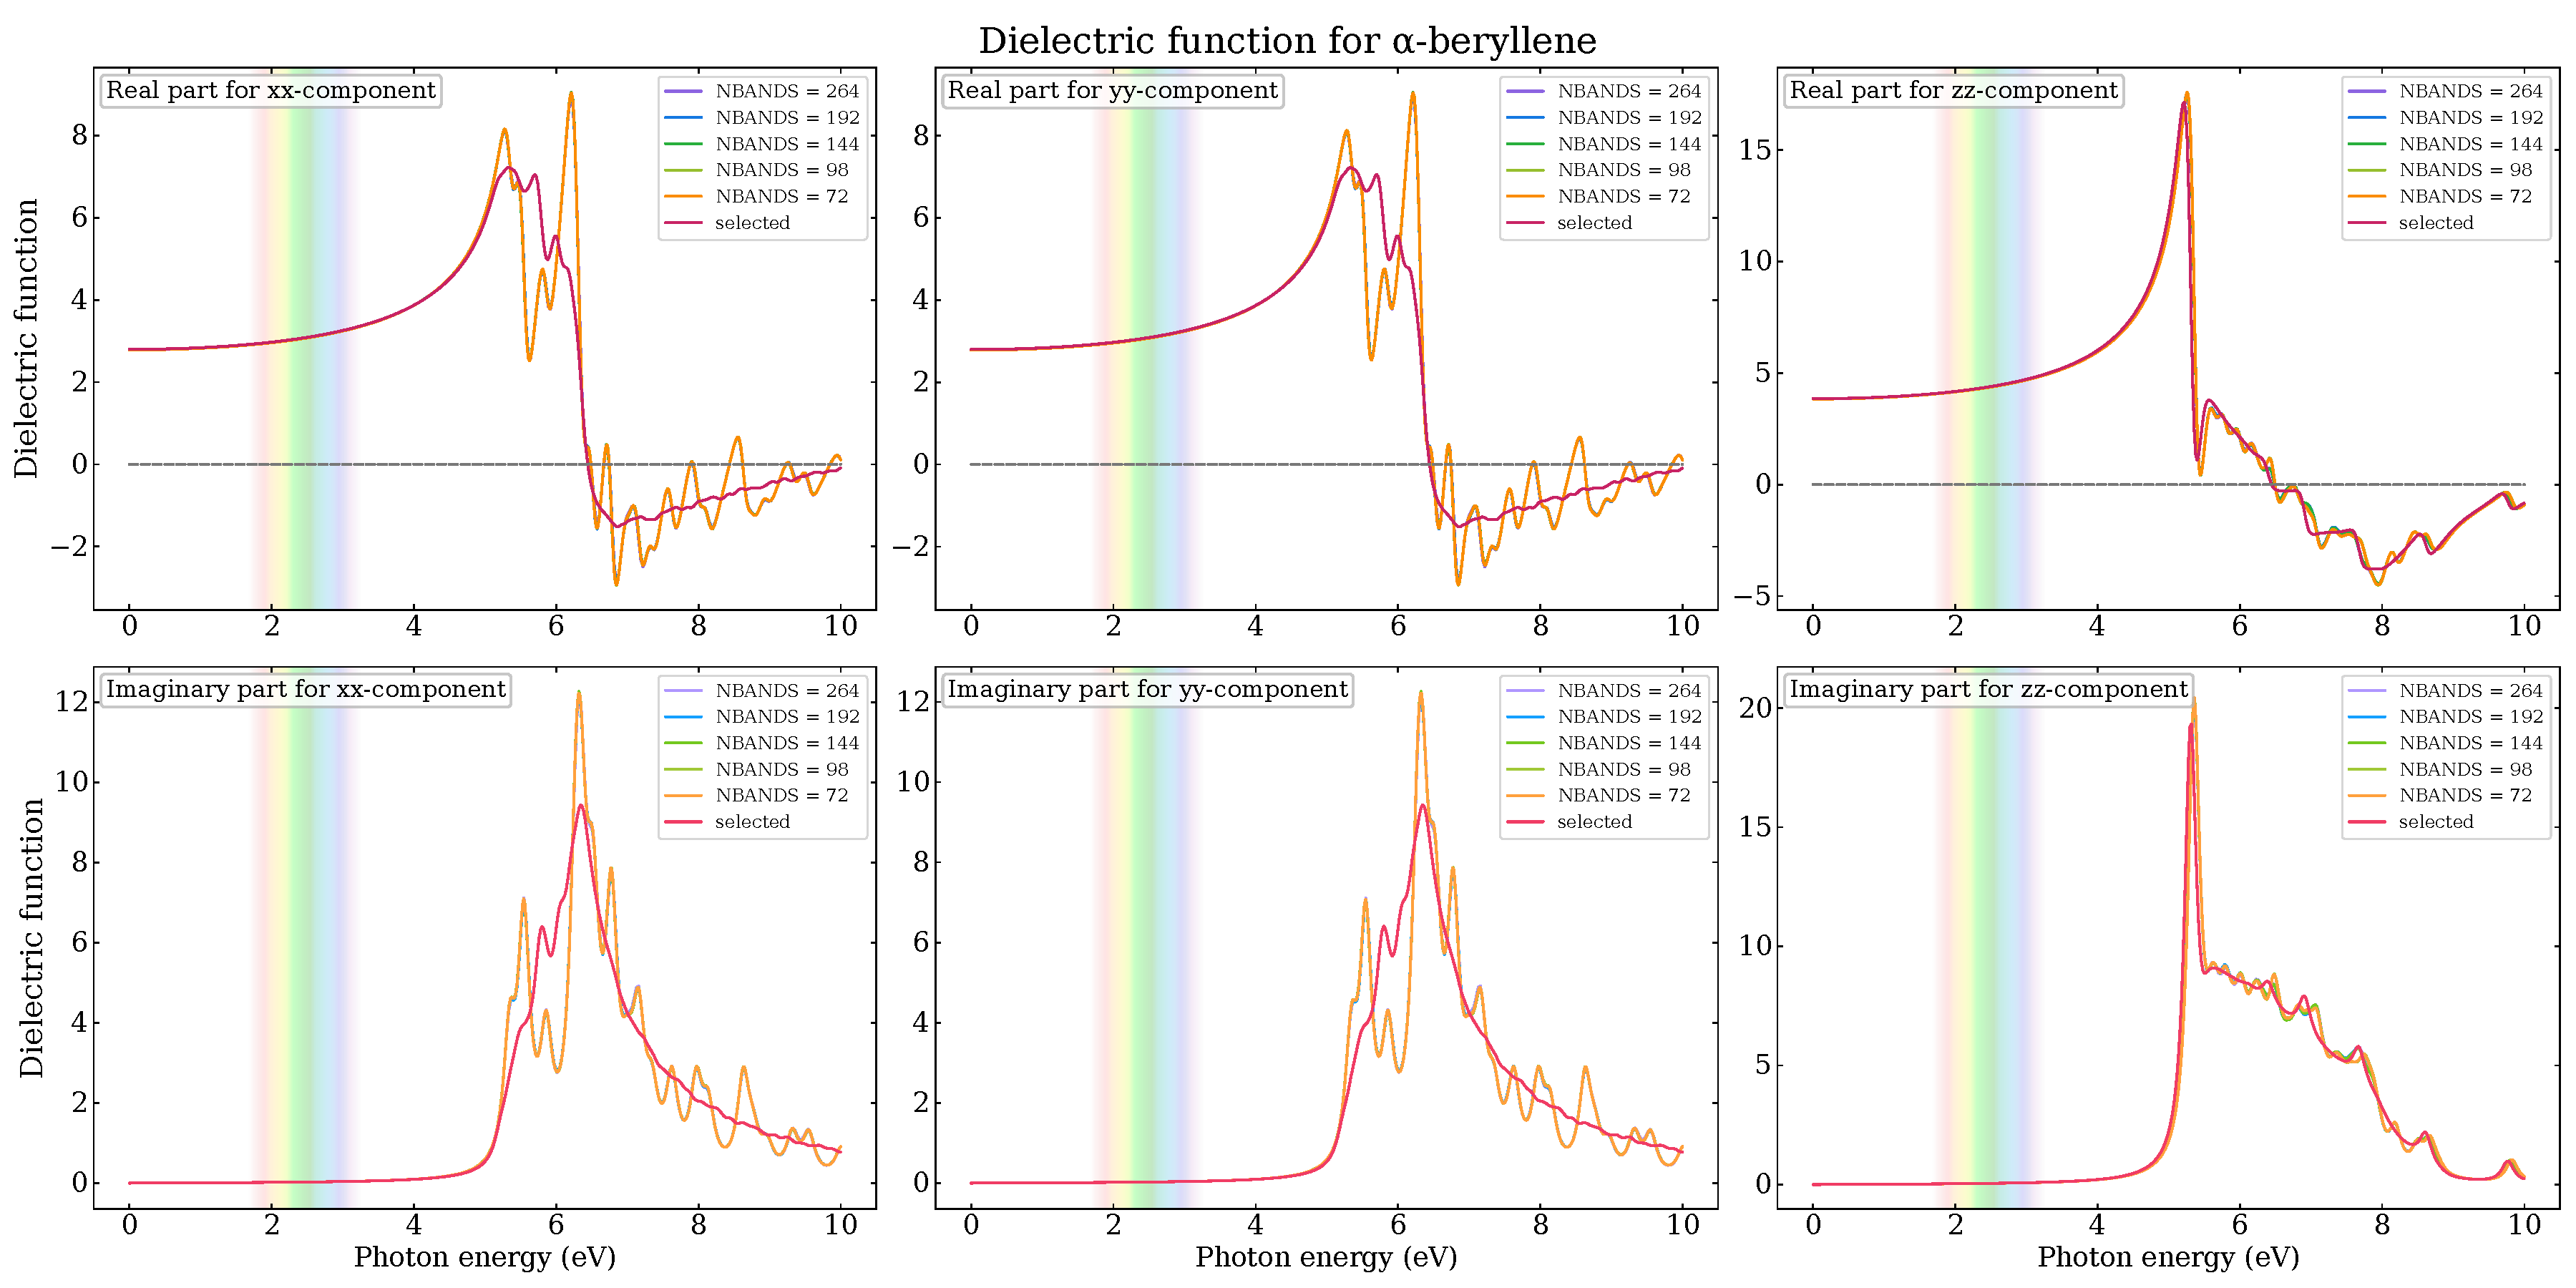
\includegraphics[width=1.0\linewidth]{figures_proj3/convergence_dielectric_nbands_alpha-beryllene_thesis.pdf}
\caption{Real and imaginary parts of the dielectric function for $\alpha$-beryllene,
calculated with different total numbers of bands.}
\label{fig:proj3_alpha_dielectric_nbands_convergence}
\end{figure}

\begin{figure}[!htbp]
\centering
    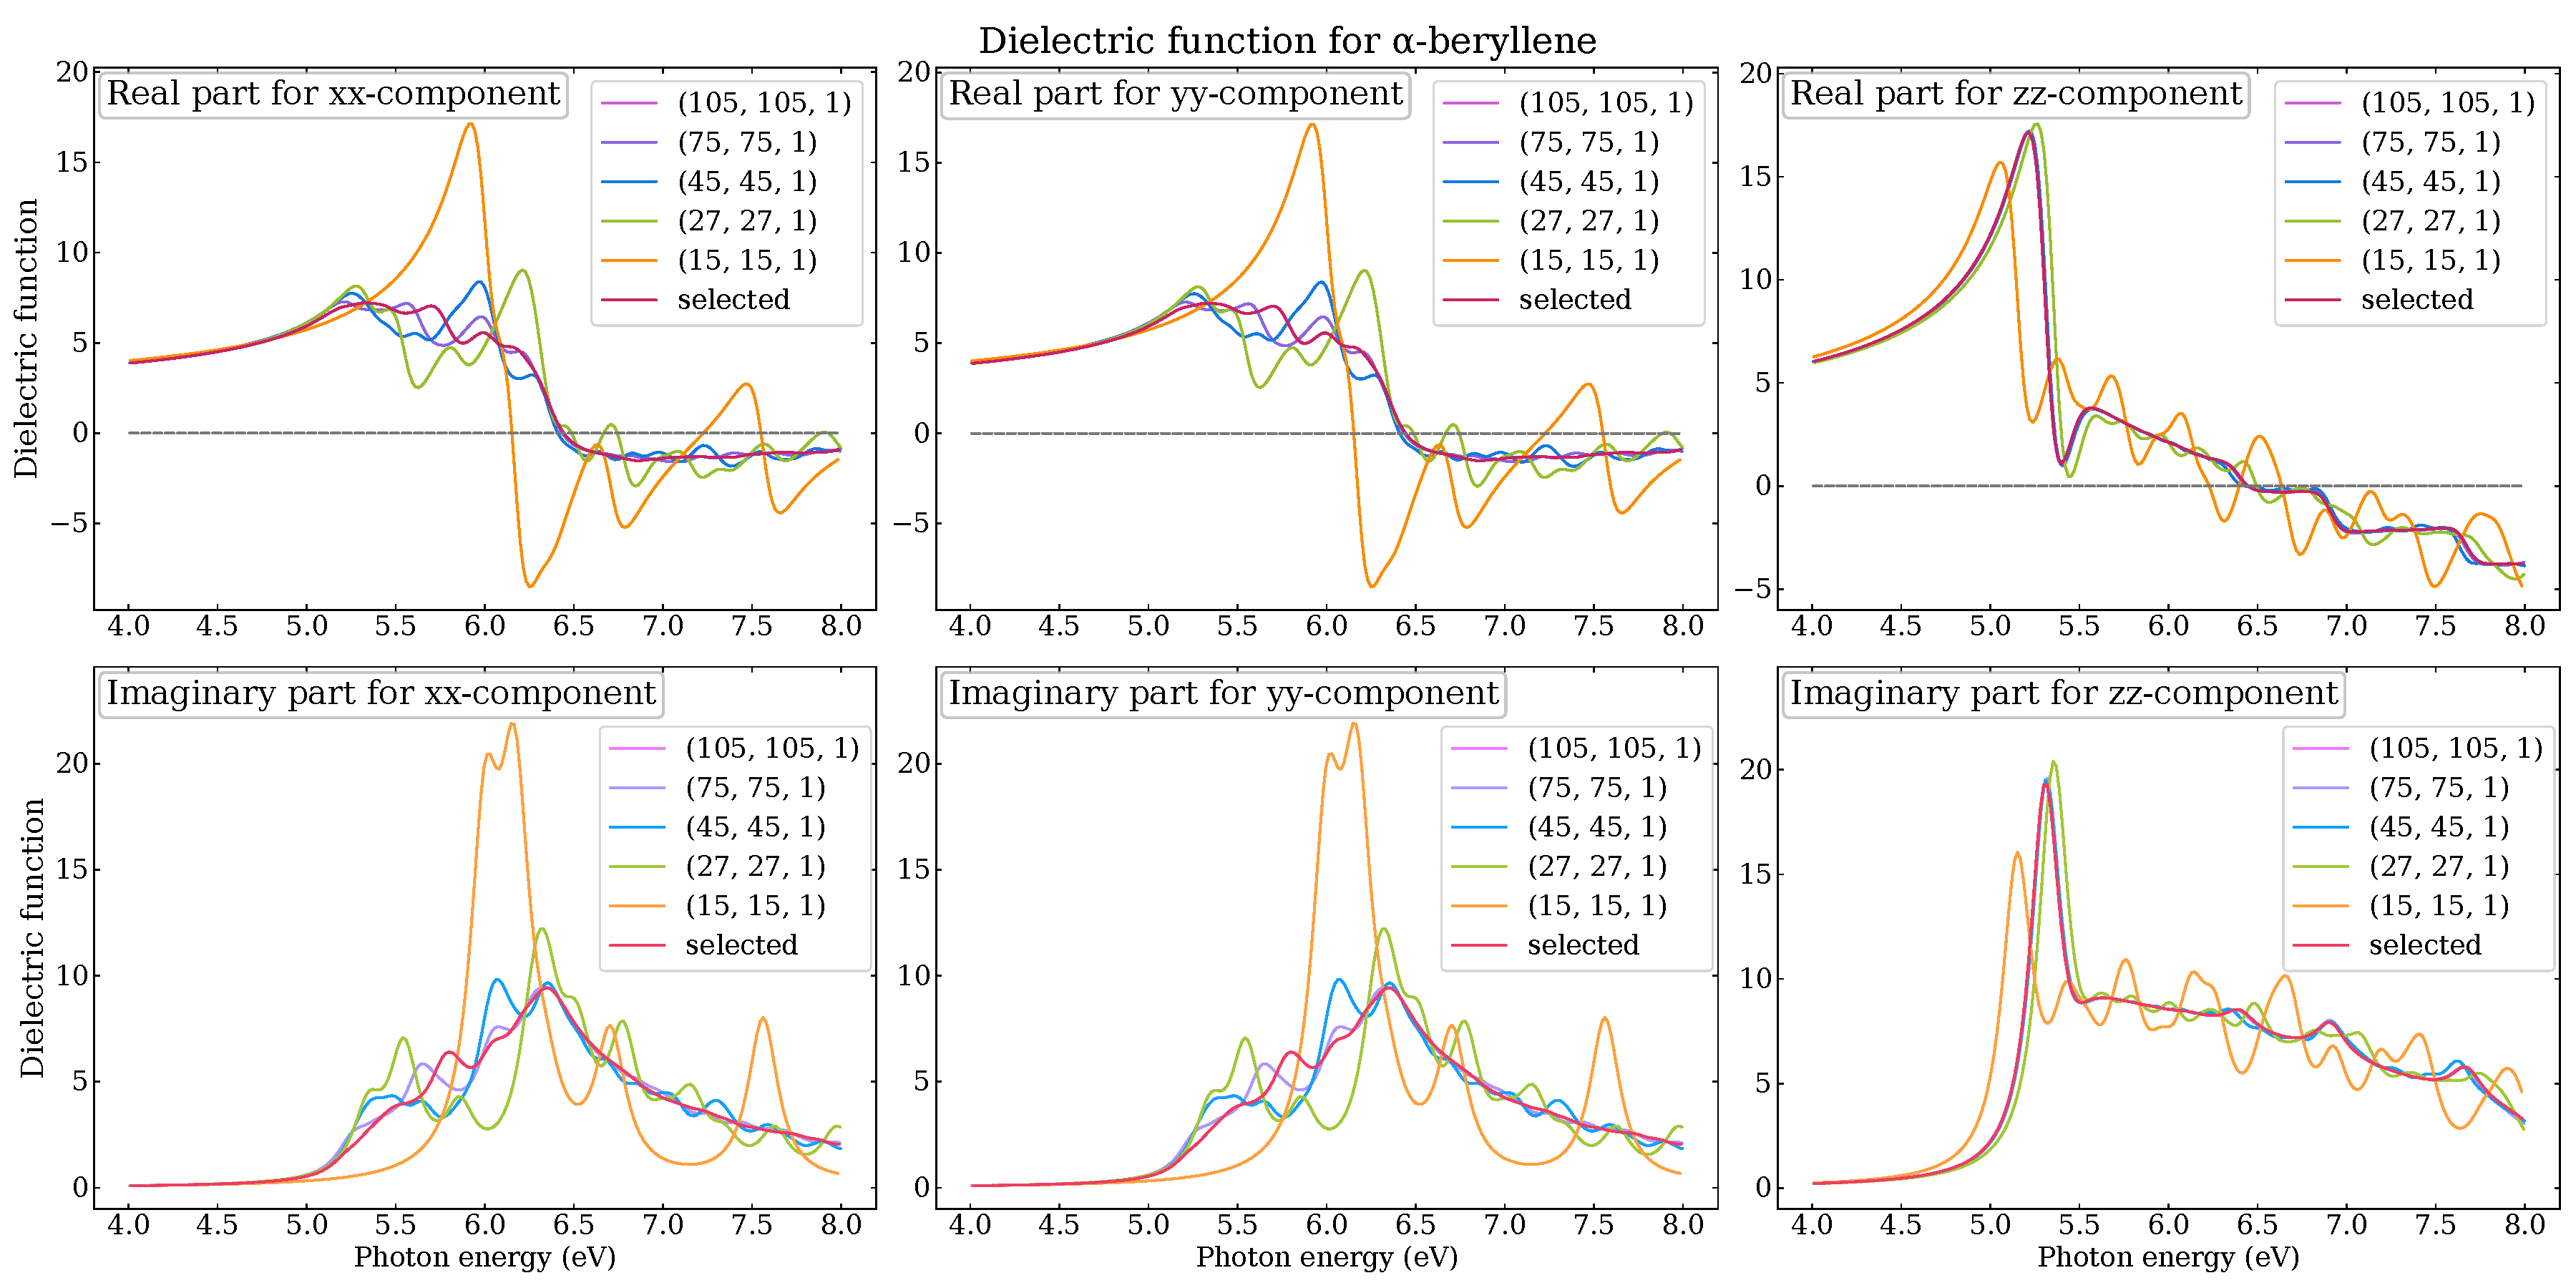
\includegraphics[width=1.0\linewidth]{figures_proj3/convergence_dielectric_kpoints_alpha-beryllene_thesis.pdf}
\caption{Real and imaginary parts of the dielectric function for $\alpha$-beryllene,
calculated with different k-point meshes.}
\label{fig:proj3_alpha_dielectric_kpoint_convergence}
\end{figure}

\begin{figure}[!htbp]
\centering
    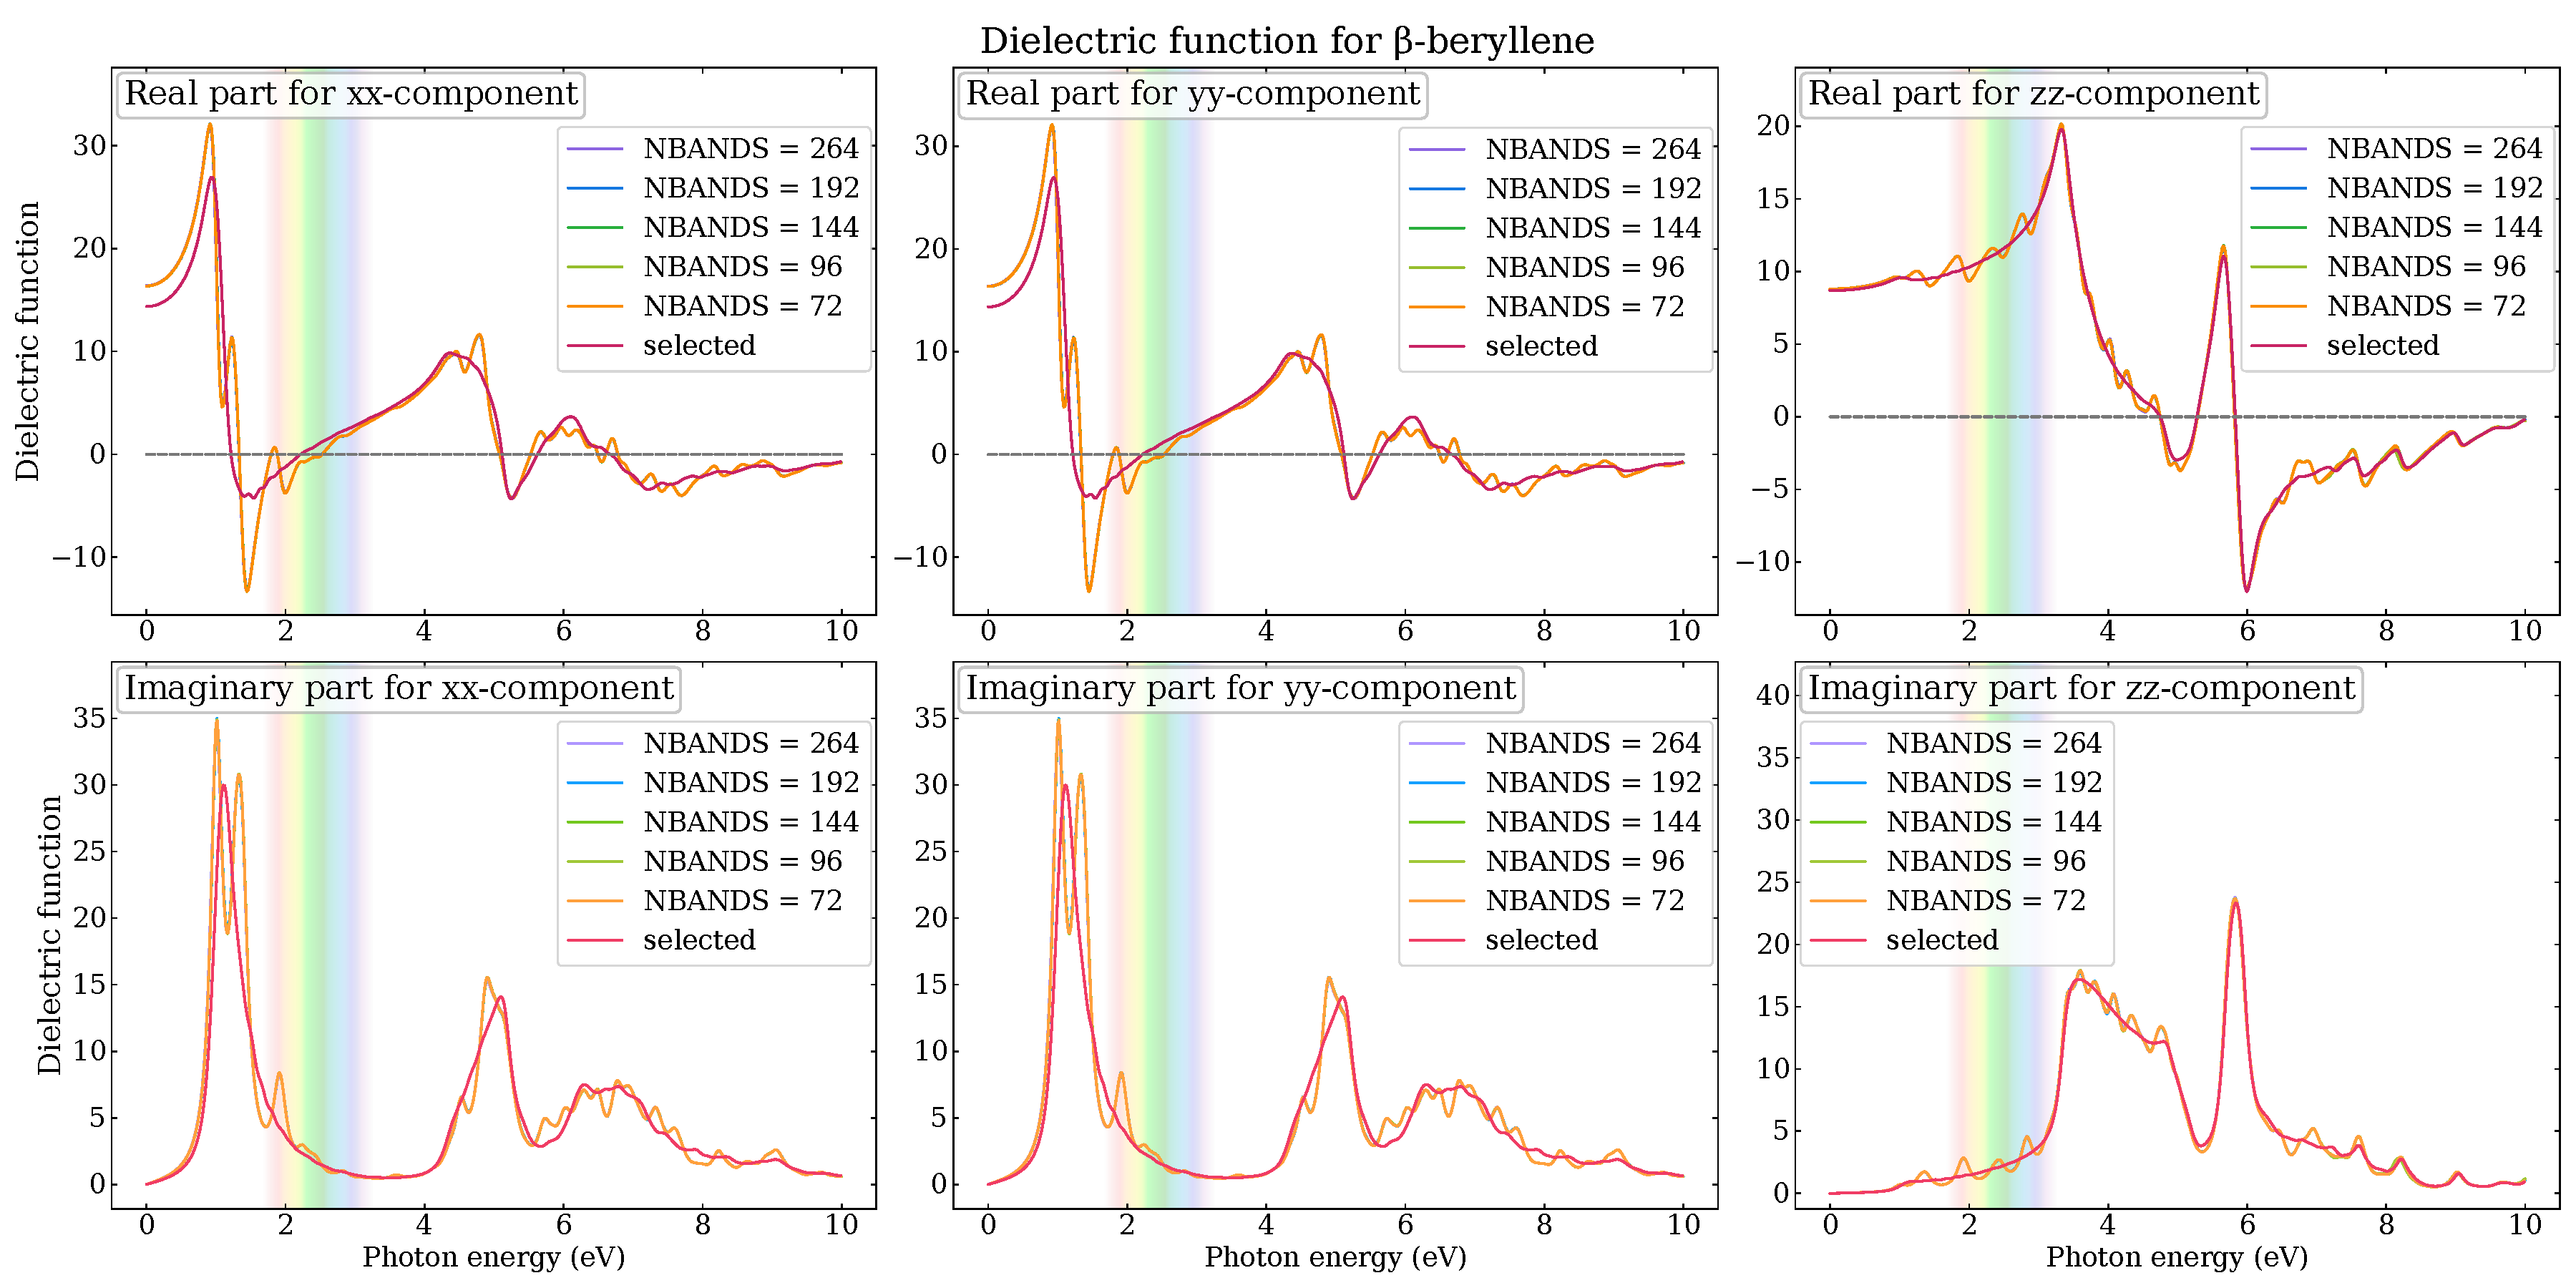
\includegraphics[width=1.0\linewidth]{figures_proj3/convergence_dielectric_nbands_beta-beryllene_thesis.pdf}
\caption{Real and imaginary parts of the dielectric function for $\beta$-beryllene,
calculated with different total numbers of bands.}
\label{fig:proj3_beta_dielectric_nbands_convergence}
\end{figure}

\begin{figure}[!htbp]
\centering
    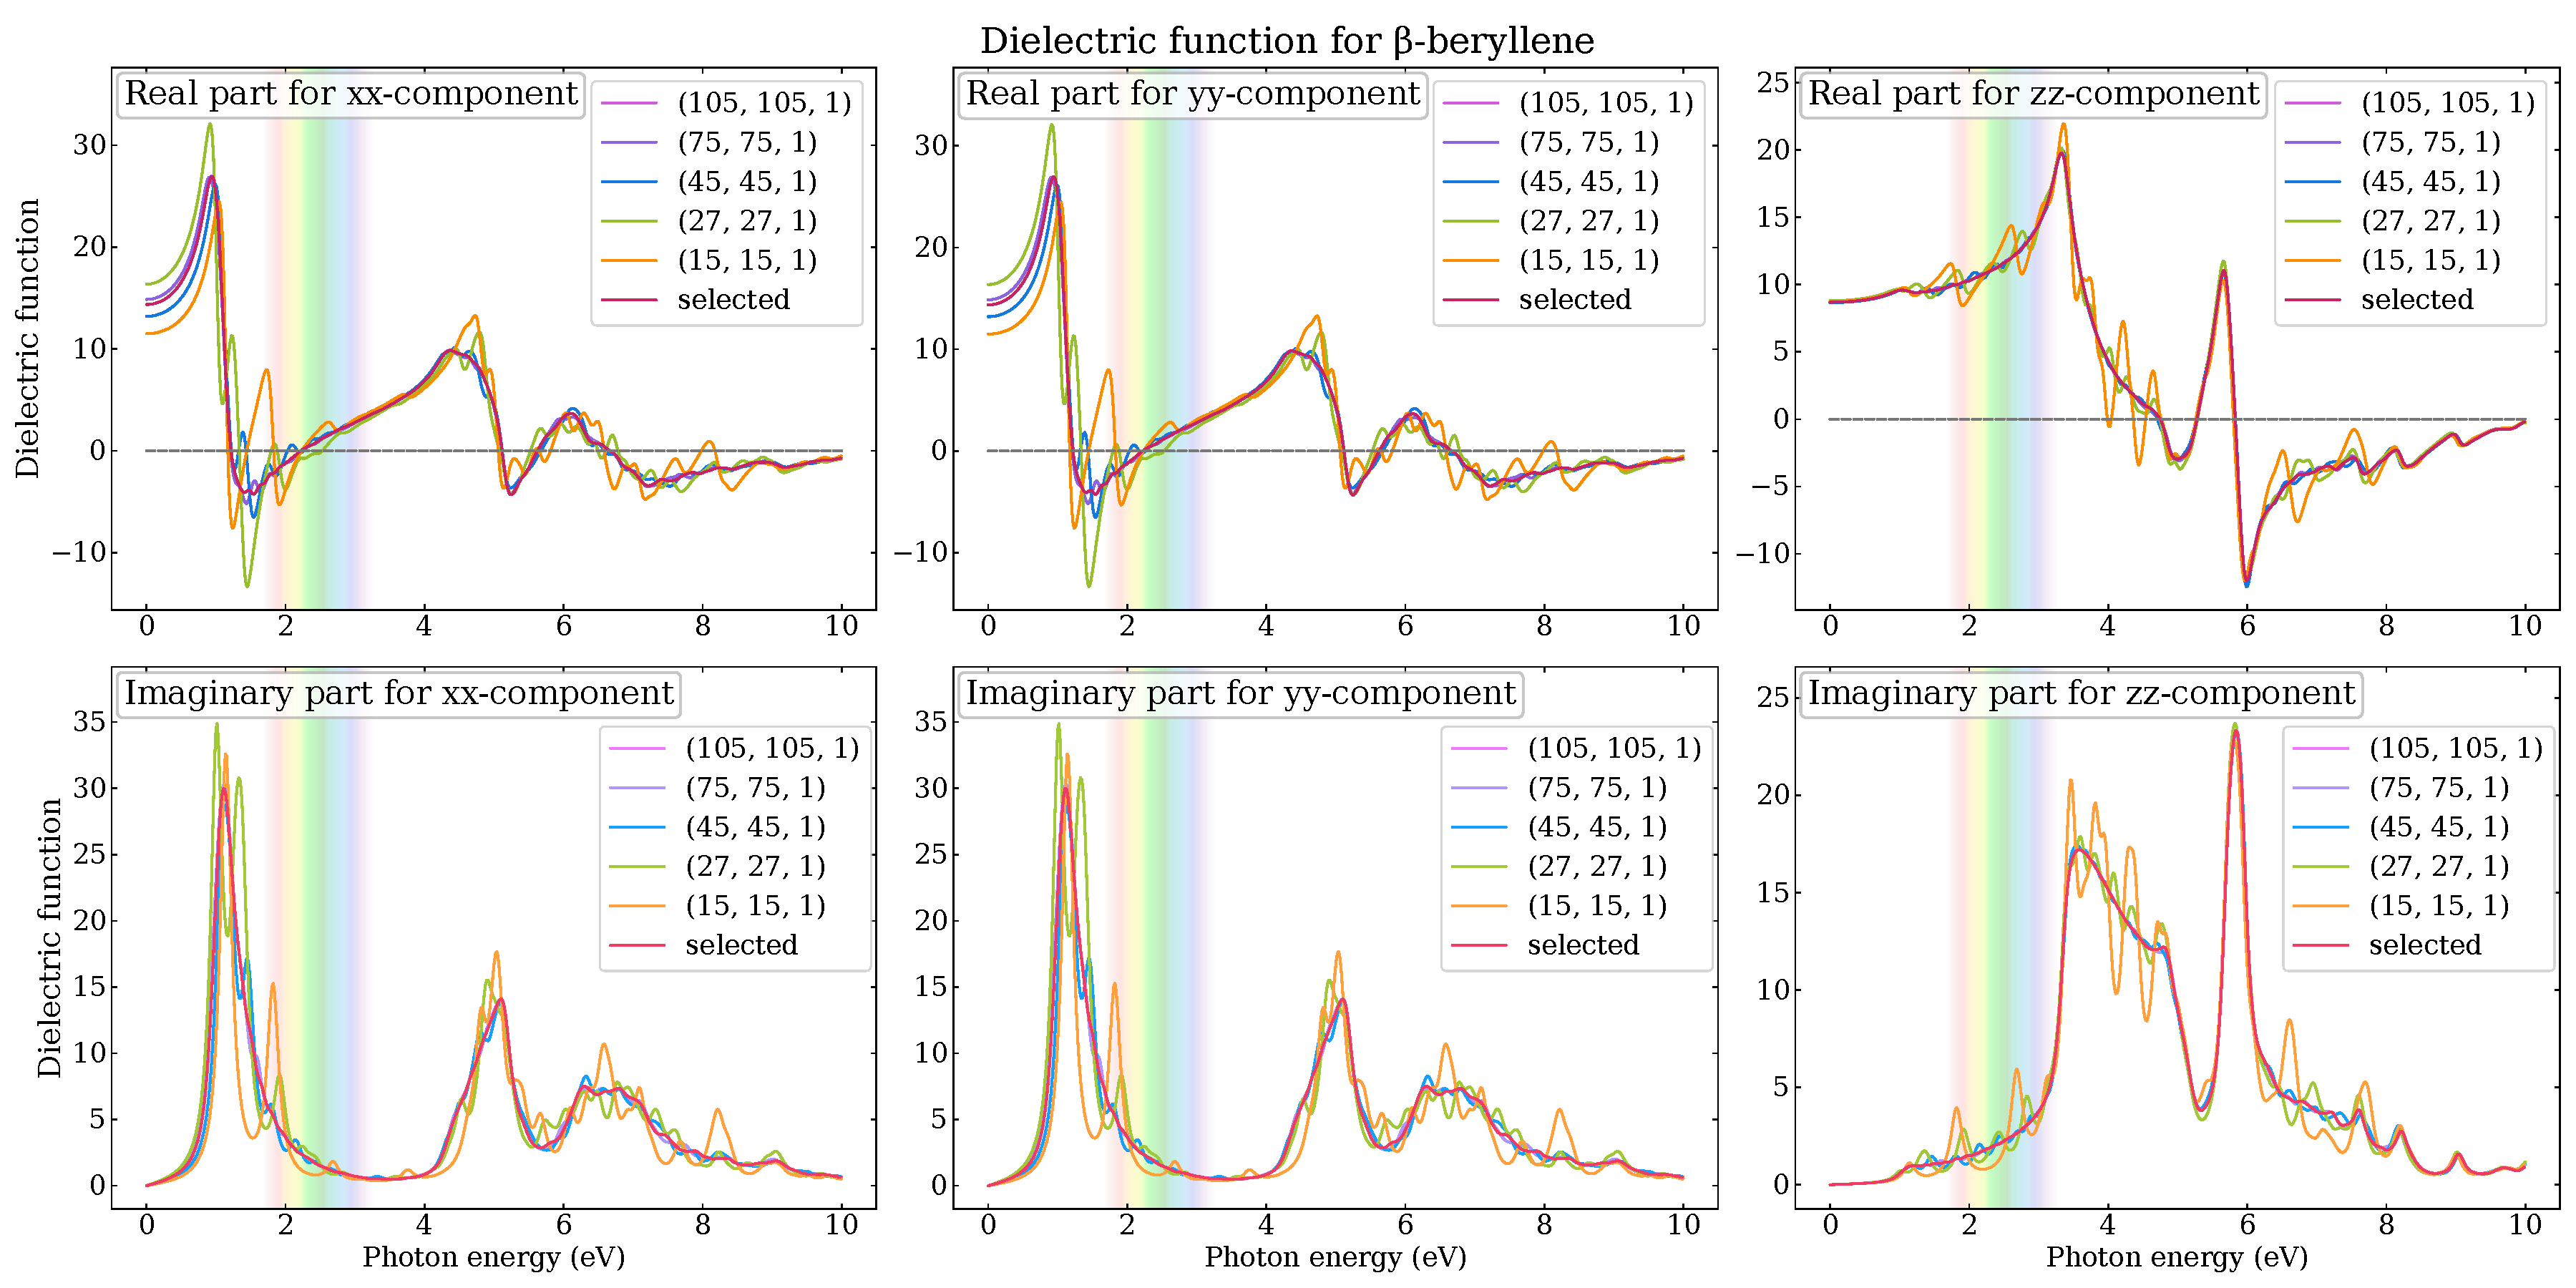
\includegraphics[width=1.0\linewidth]{figures_proj3/convergence_dielectric_kpoints_beta-beryllene_thesis.pdf}
\caption{Real and imaginary parts of the dielectric function for $\beta$-beryllene,
calculated with different k-point meshes.}
\label{fig:proj3_beta_dielectric_kpoint_convergence}
\end{figure}

\begin{figure}[!htbp]
\centering
    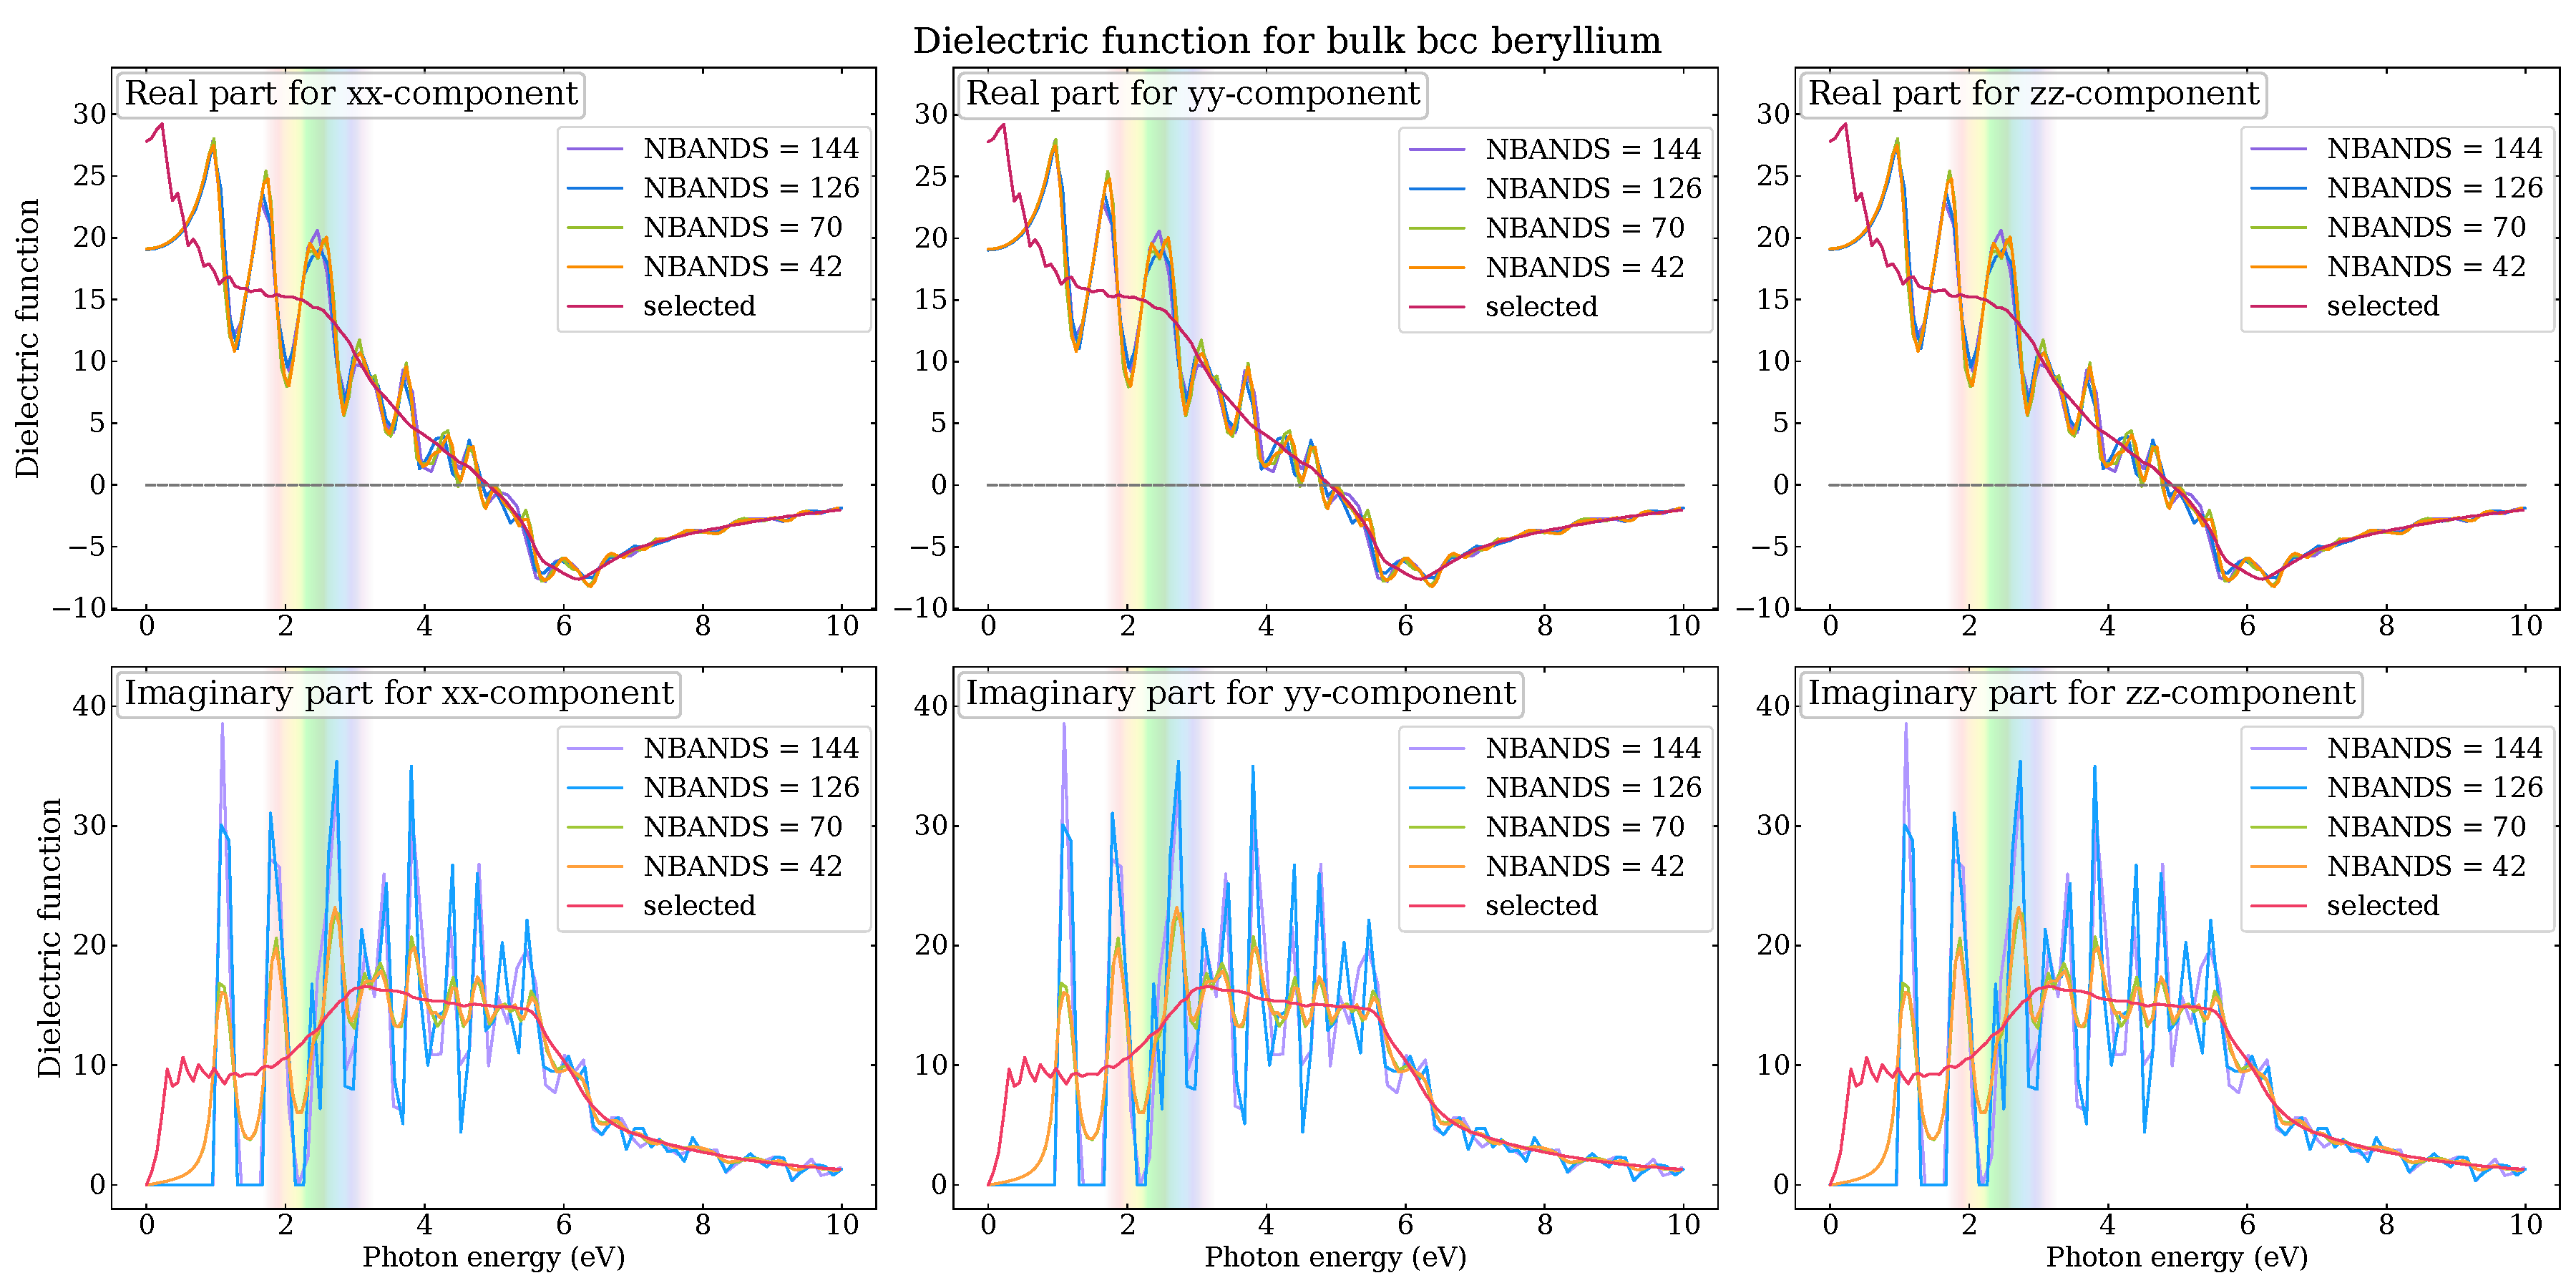
\includegraphics[width=1.0\linewidth]{figures_proj3/convergence_dielectric_nbands_bcc-beryllium_thesis.pdf}
\caption{Real and imaginary parts of the dielectric function for bulk bcc beryllium,
calculated with different total numbers of bands.}
\label{fig:proj3_bcc_dielectric_nbands_convergence}
\end{figure}

\begin{figure}[!htbp]
\centering
    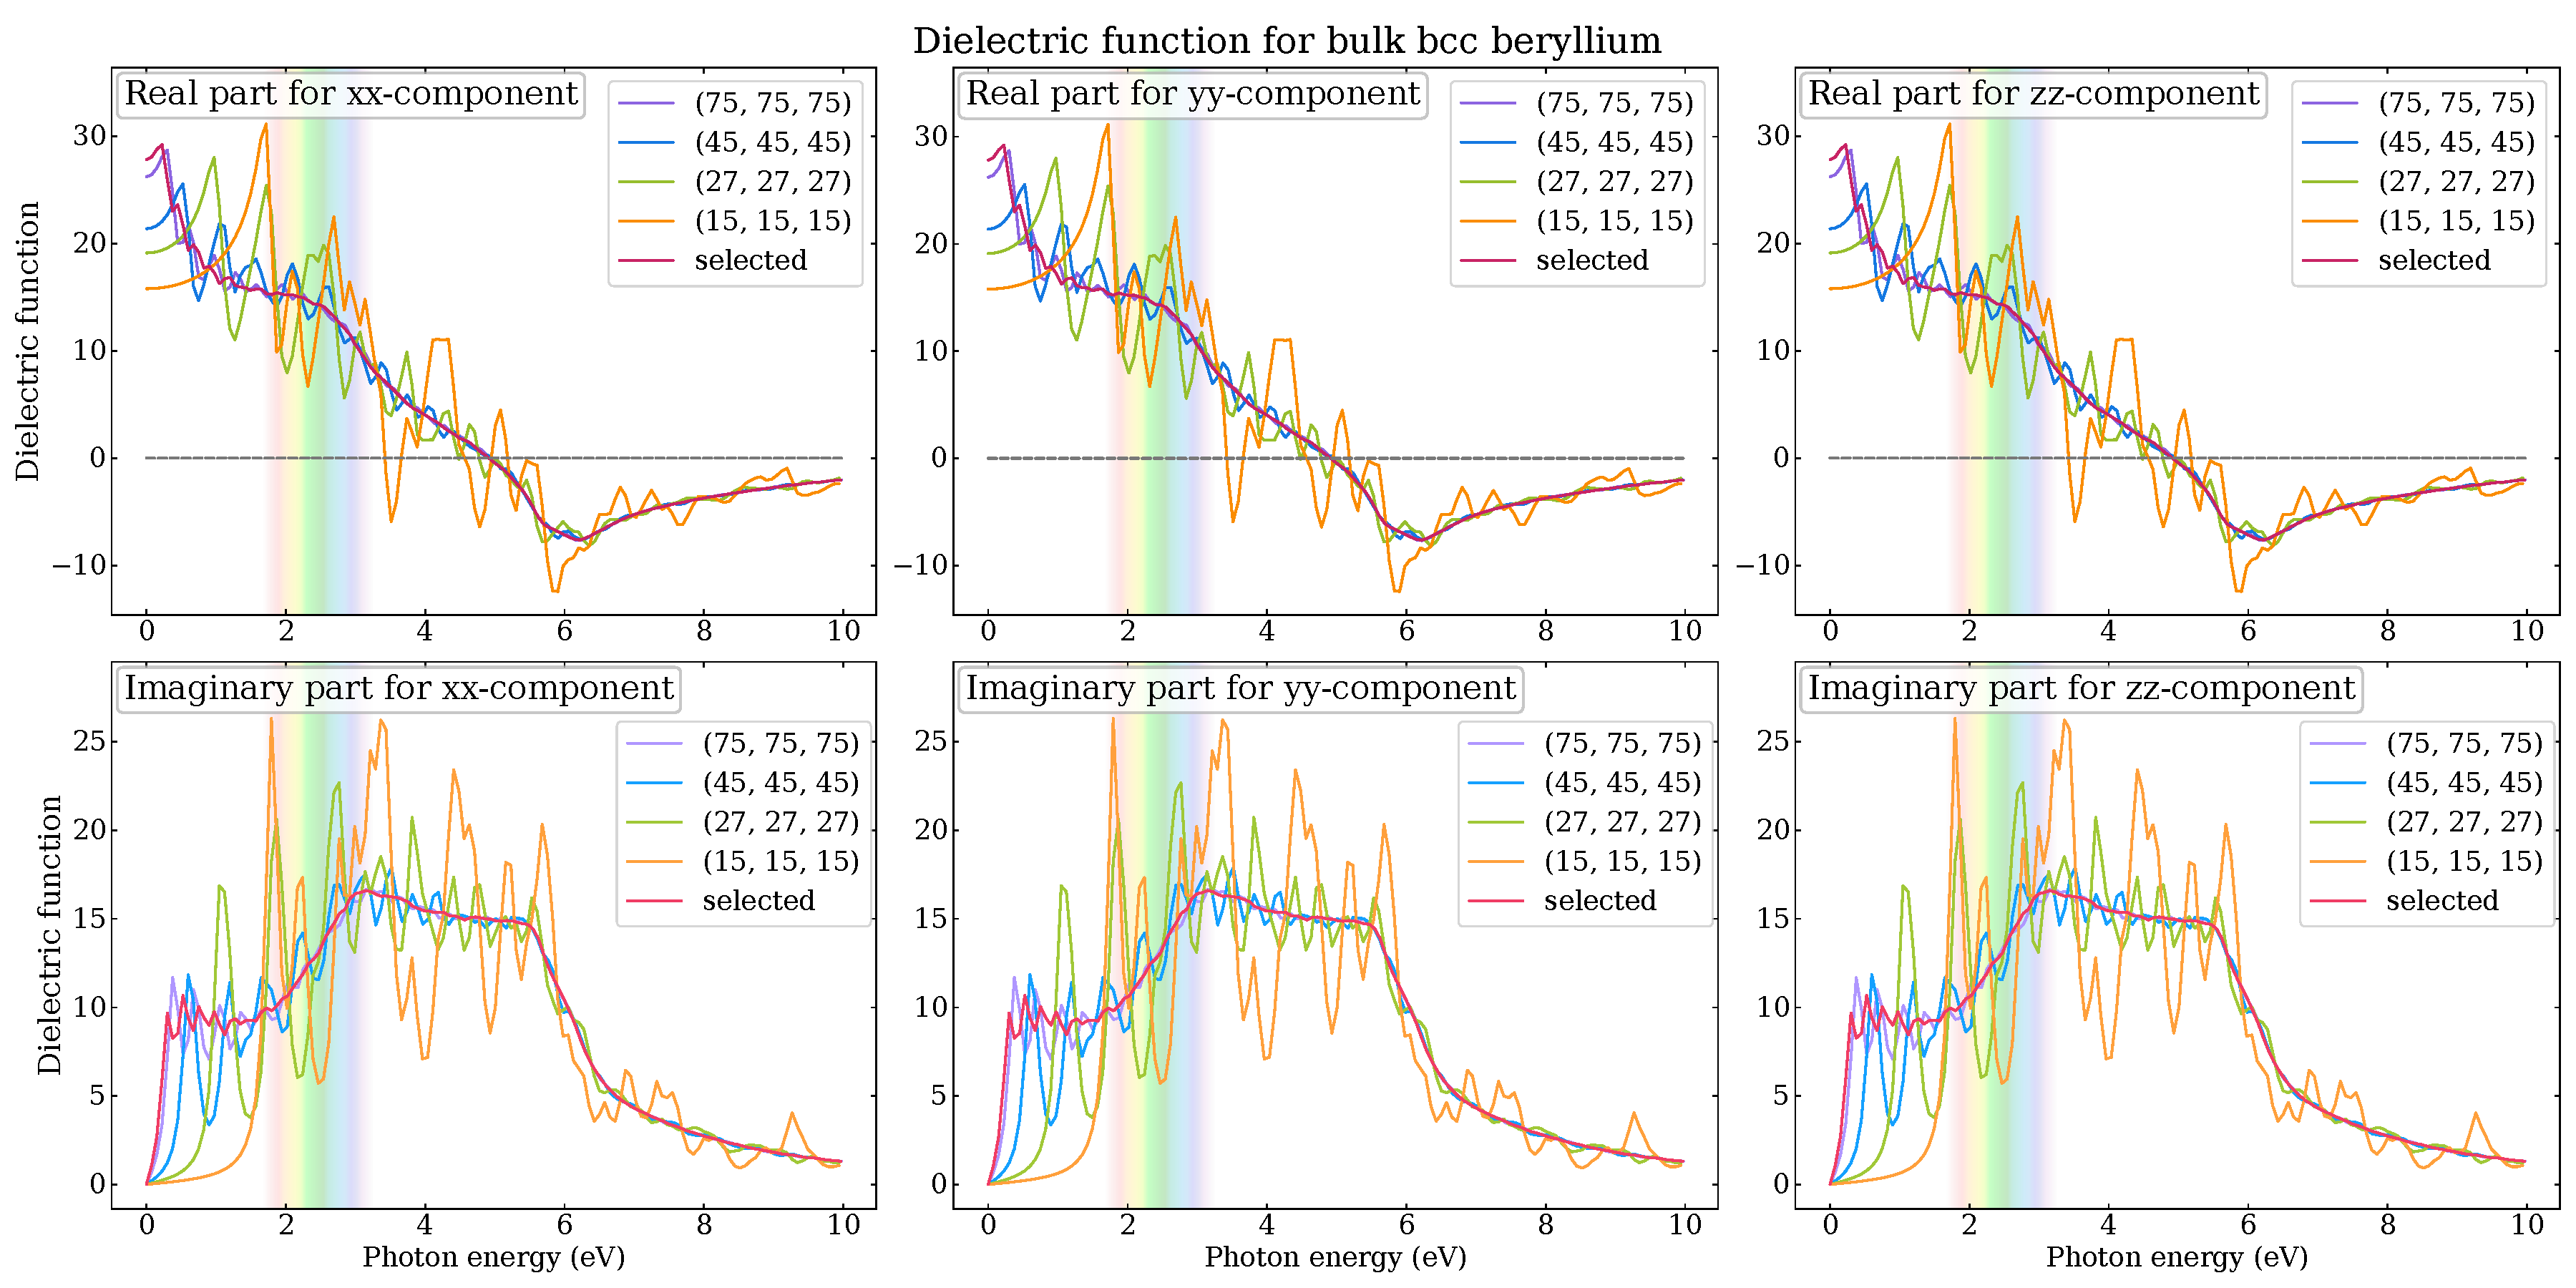
\includegraphics[width=1.0\linewidth]{figures_proj3/convergence_dielectric_kpoints_bcc-beryllium_thesis.pdf}
\caption{Real and imaginary parts of the dielectric function for bulk bcc beryllium,
calculated with different k-point meshes.}
\label{fig:proj3_bcc_dielectric_kpoint_convergence}
\end{figure}

\begin{figure}[!htbp]
\centering
    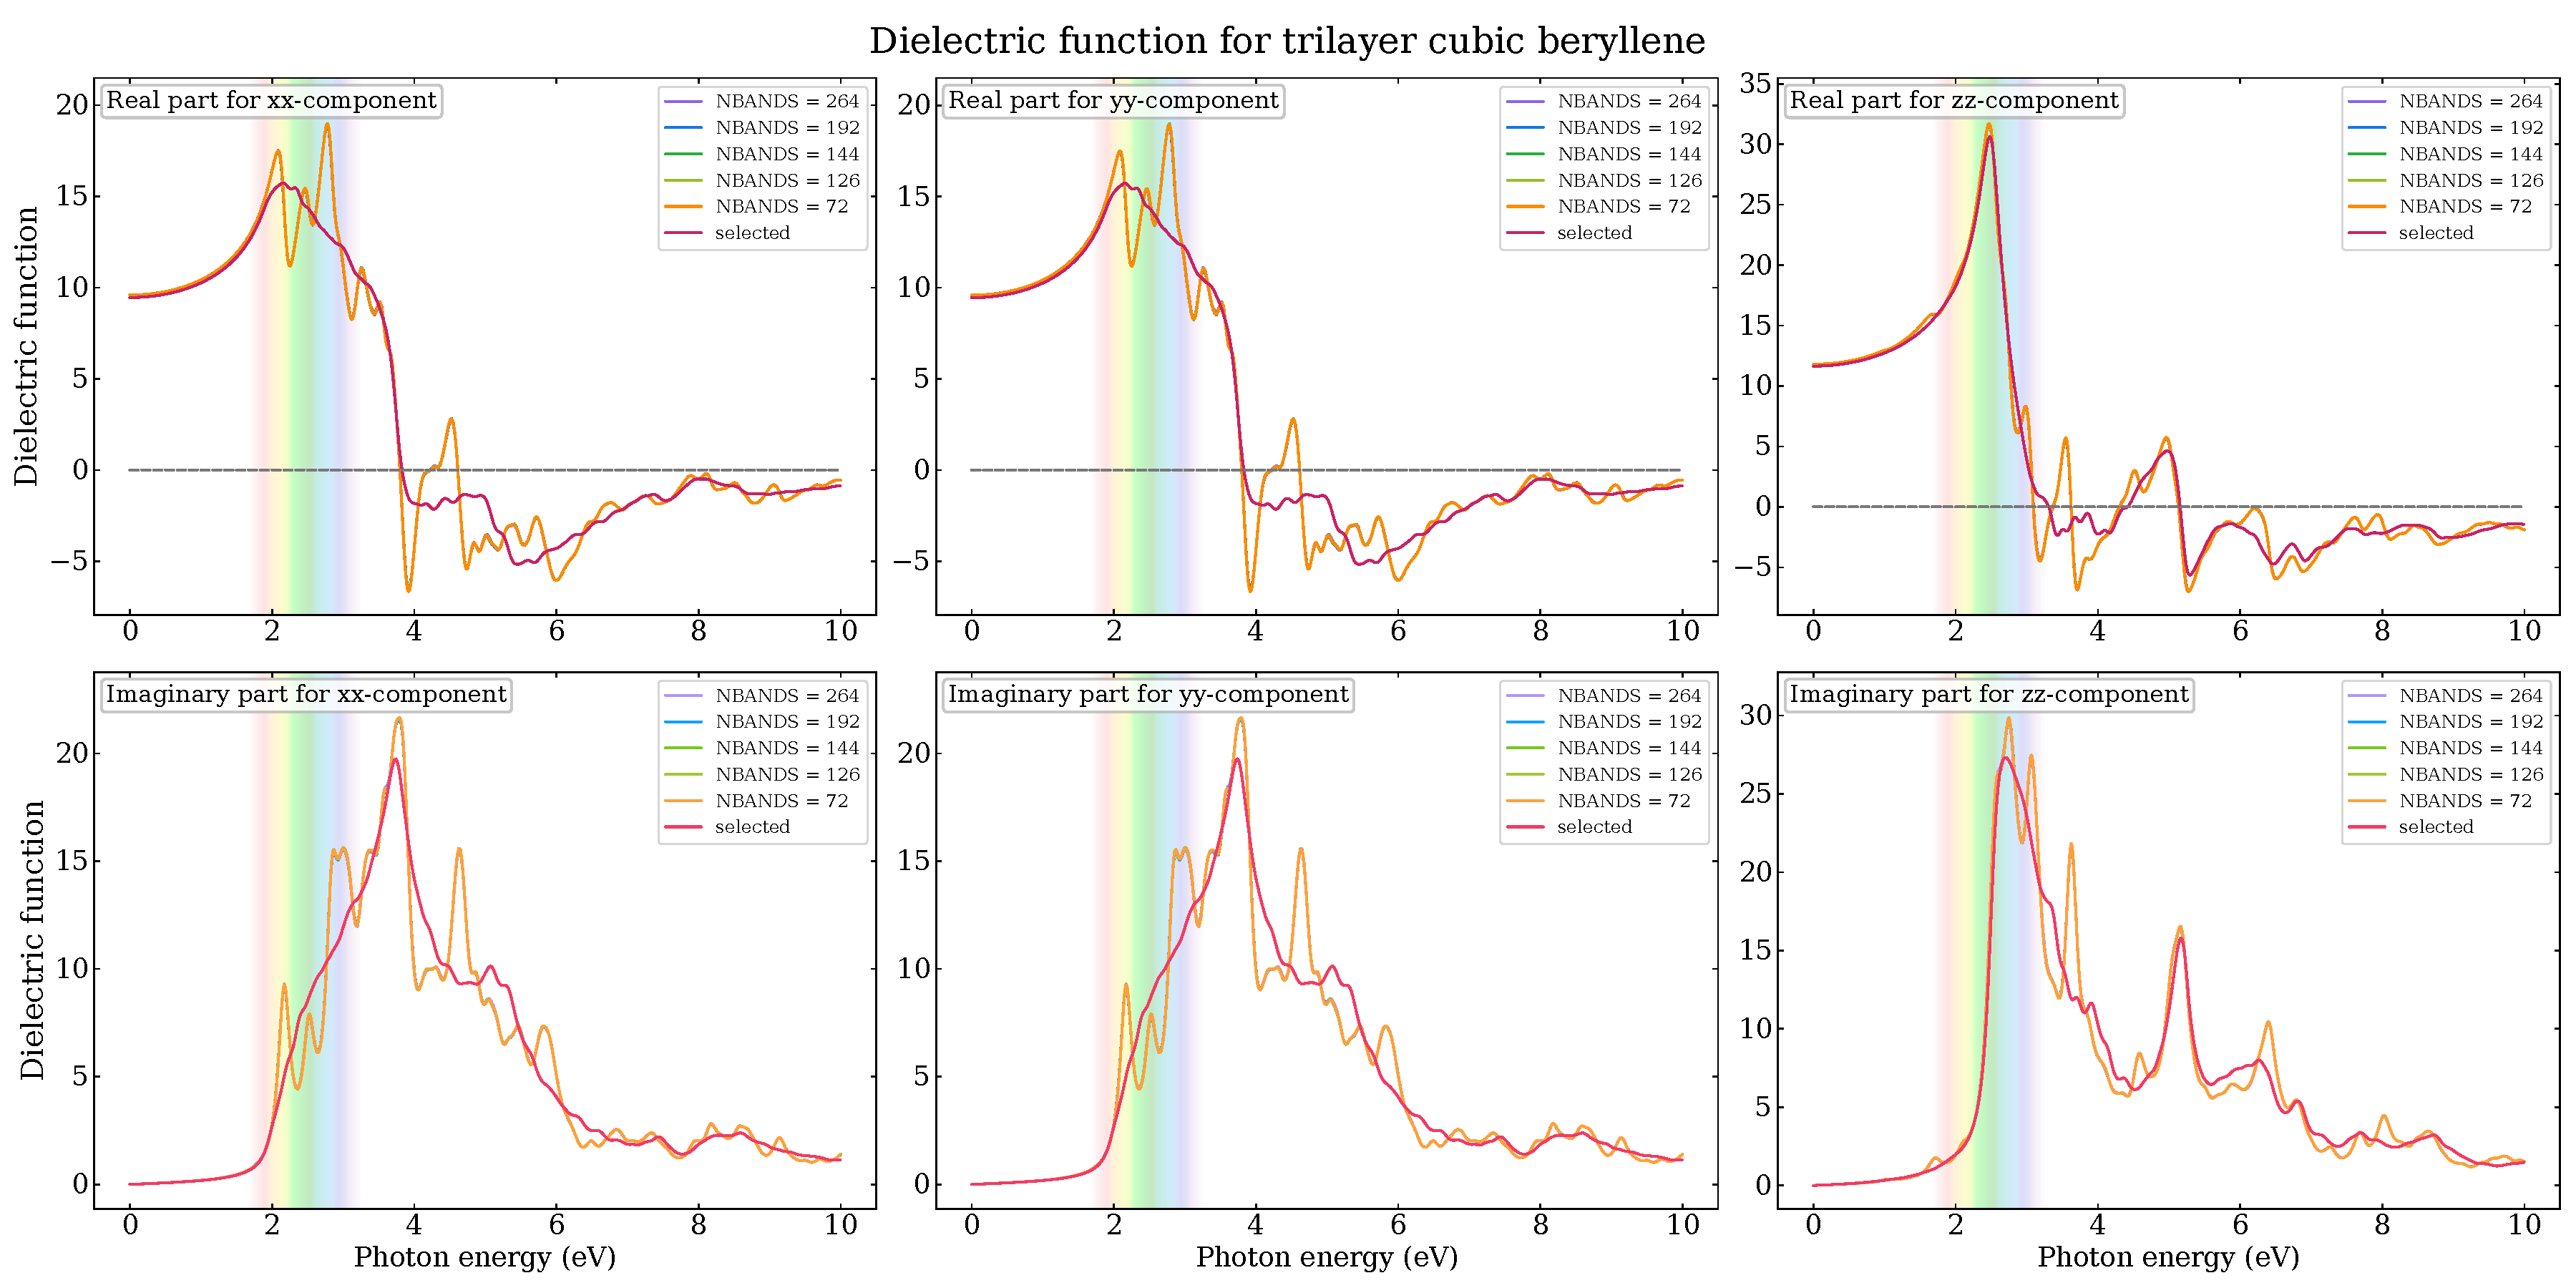
\includegraphics[width=1.0\linewidth]{figures_proj3/convergence_dielectric_nbands_cubic-beryllene-trilayer_thesis.pdf}
\caption{Real and imaginary parts of the dielectric function for trilayer cubic beryllene,
calculated with different total numbers of bands.}
\label{fig:proj3_cubic_dielectric_nbands_convergence}
\end{figure}

\begin{figure}[!htbp]
\centering
    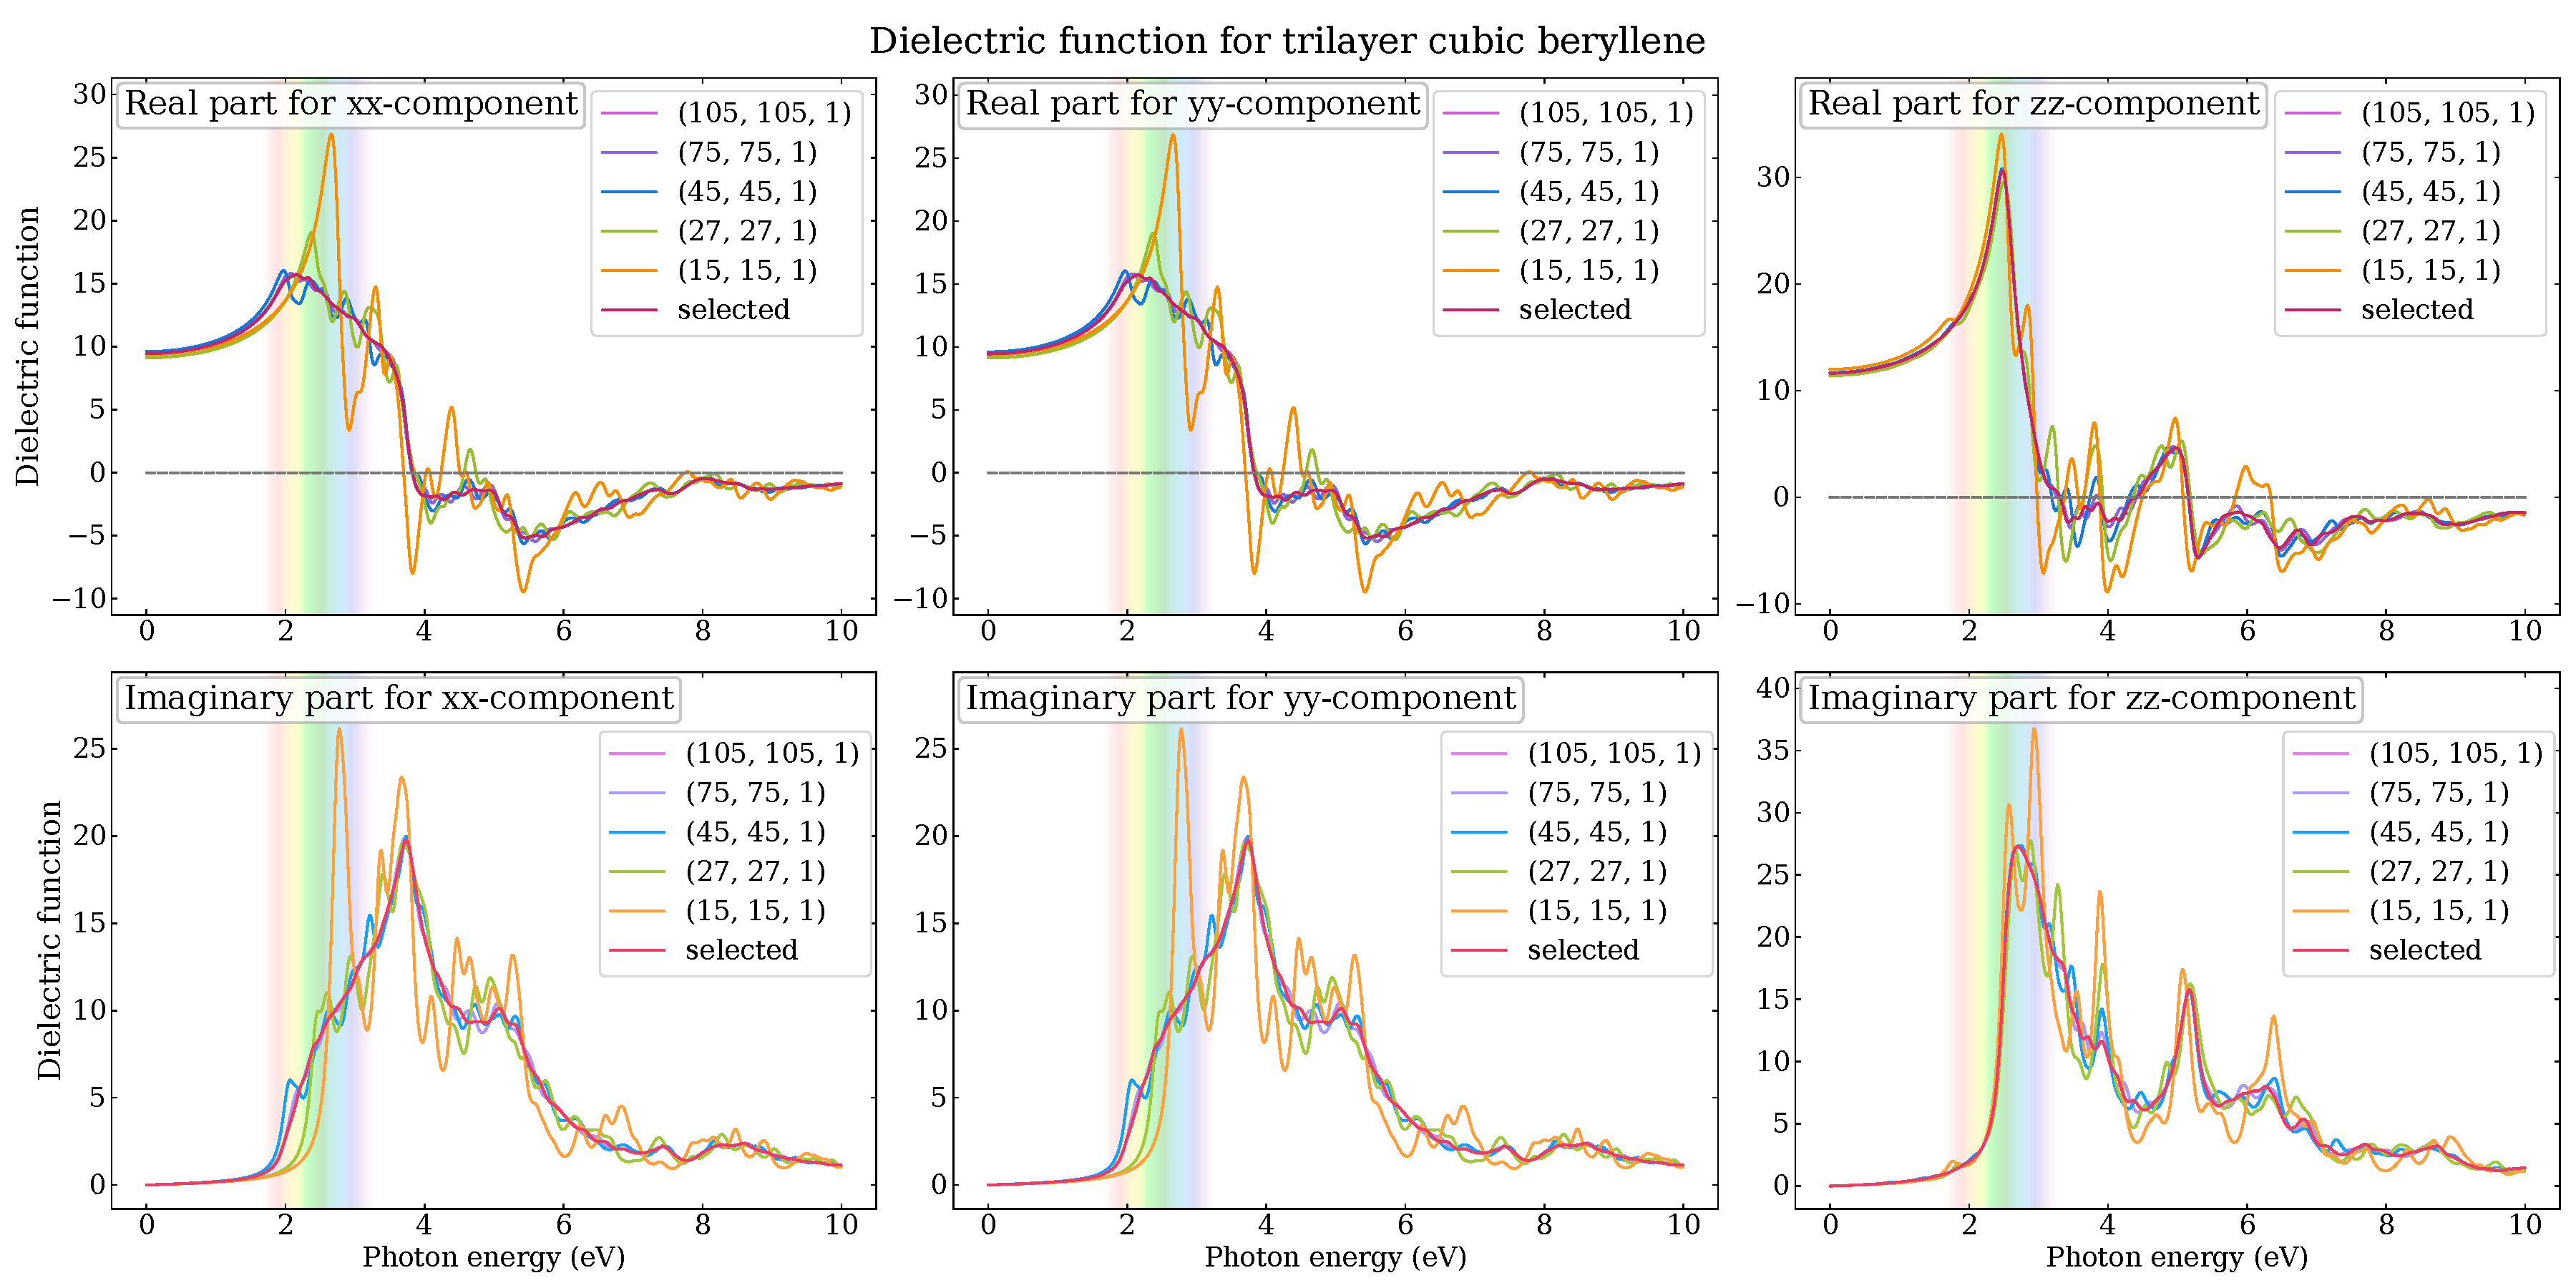
\includegraphics[width=1.0\linewidth]{figures_proj3/convergence_dielectric_kpoints_cubic-beryllene-trilayer_thesis.pdf}
\caption{Real and imaginary parts of the dielectric function for trilayer cubic beryllene,
calculated with different k-point meshes.}
\label{fig:proj3_cubic_dielectric_kpoint_convergence}
\end{figure}

\FloatBarrier
\subsection*{Phonon dispersions, Brillouin zones, and band structures}

Figures~\ref{fig:proj3_phonon_dispersion} and~\ref{fig:proj3_band_structures} show the phonon dispersions and electronic bands of $\alpha$-beryllene, $\beta$-beryllene, and bulk hcp and bcc beryllium.
The phonon force constants come from PBE without D3.
For the electronic bands, we use the fixed PBE geometries and the energy references in section~\ref{3_methods}.
Bulk bcc beryllium has an imaginary frequency of $3.90\mathrm{i}$~\unit{\tera\hertz} at the $\mathrm{N}$ point, which is commensurate with the $4 \times 4 \times 4$ supercell.
The harmonic instability is consistent with the anharmonic stabilization of this phase at high temperatures.

Figure~\ref{fig:proj3_brillouin_zones} shows the reciprocal-space paths for the hexagonal and distorted hexagonal cells.
For 1H-$\beta$-beryllene and 2H-$\beta$-beryllene, the bands and phonon dispersions follow panel~(b).
The respective angles between the lattice vectors are approximately \qty{117}{\degree} and \qty{133}{\degree}.
The distorted zones retain corners $\mathrm{K}$ and $\mathrm{K}'$ derived from the hexagonal zone.
The points $\mathrm{X}$, $\mathrm{Y}$, and $\mathrm{M}$ derive from its three equivalent $\mathrm{M}$ points.
The two cells have strict symmetries $P1$ and $P\bar{1}$, respectively.
Modulo a reciprocal lattice vector, time reversal relates the two halves of each zone edge across its midpoint.
The path includes one half for each of the three edge directions.
At a positional tolerance of \qty{1e-3}{\angstrom}, the two cells have $Cm$ and $C2/m$ symmetry, respectively.
The higher symmetry relates $\Gamma$--$\mathrm{Y}$ to $\Gamma$--$\mathrm{M}$ in 1H-$\beta$-beryllene and $\Gamma$--$\mathrm{X}$ to $\Gamma$--$\mathrm{Y}$ in 2H-$\beta$-beryllene.
The calculated PBE bands along each pair of lines differ by at most \qty{3.3}{\milli\electronvolt} and \qty{7.3}{\milli\electronvolt}, respectively.

\begin{figure}[!htbp]
\centering
\begin{tabular}{@{}cc@{}}
% \begin{tabular}{cc}
    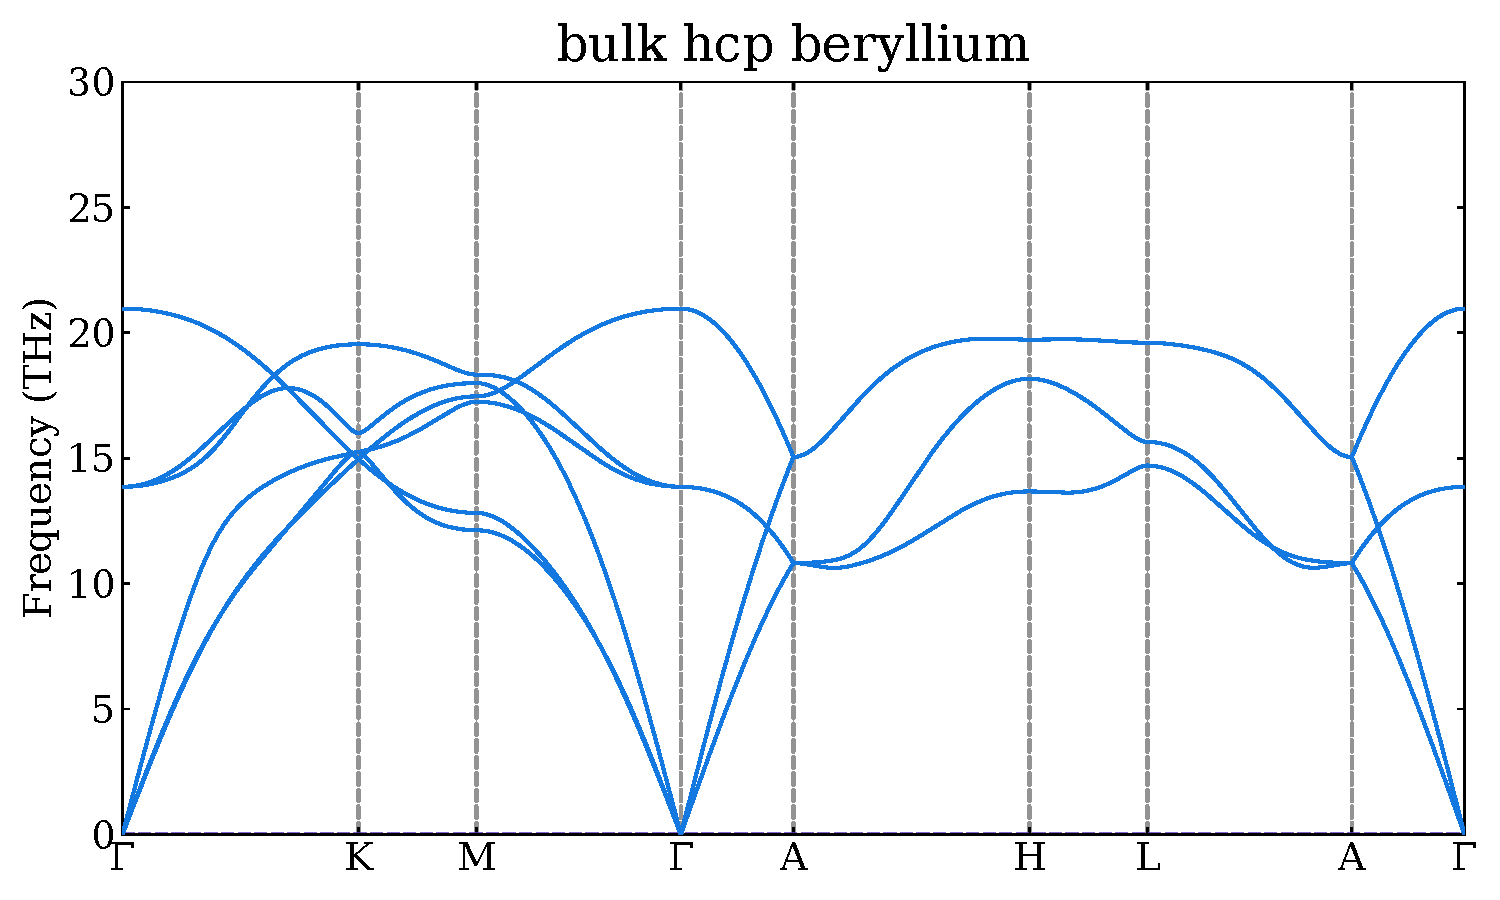
\includegraphics[width=0.40\linewidth]{figures_proj3/phonon/phonon_hcp-beryllium_thesis.pdf}&
    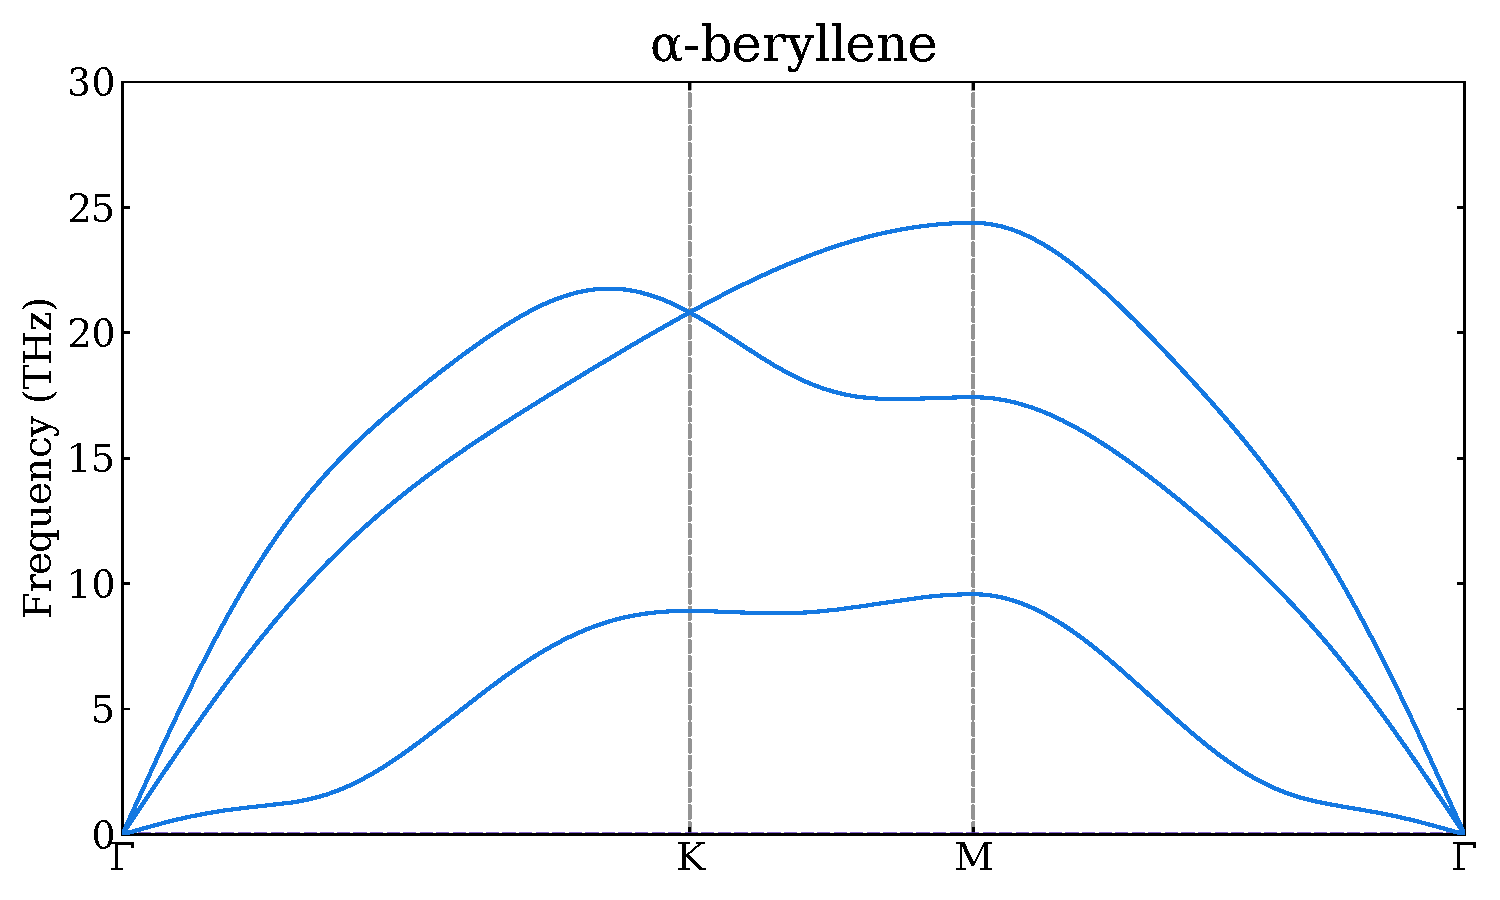
\includegraphics[width=0.40\linewidth]{figures_proj3/phonon/phonon_alpha-beryllene_thesis.pdf}\\
    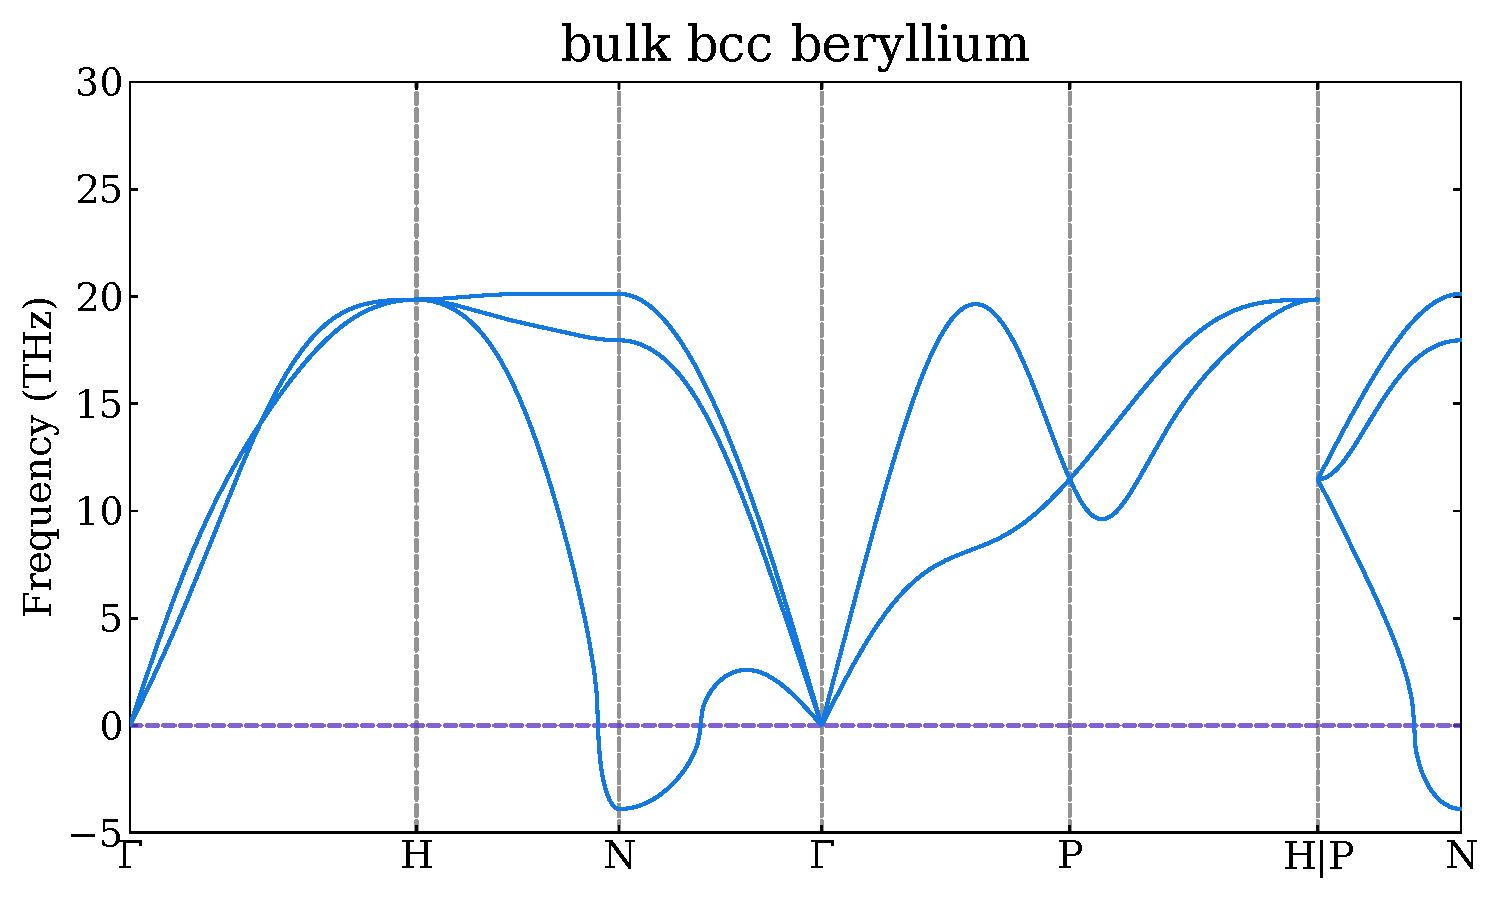
\includegraphics[width=0.40\linewidth]{figures_proj3/phonon/phonon_bcc-beryllium_thesis.pdf}&
    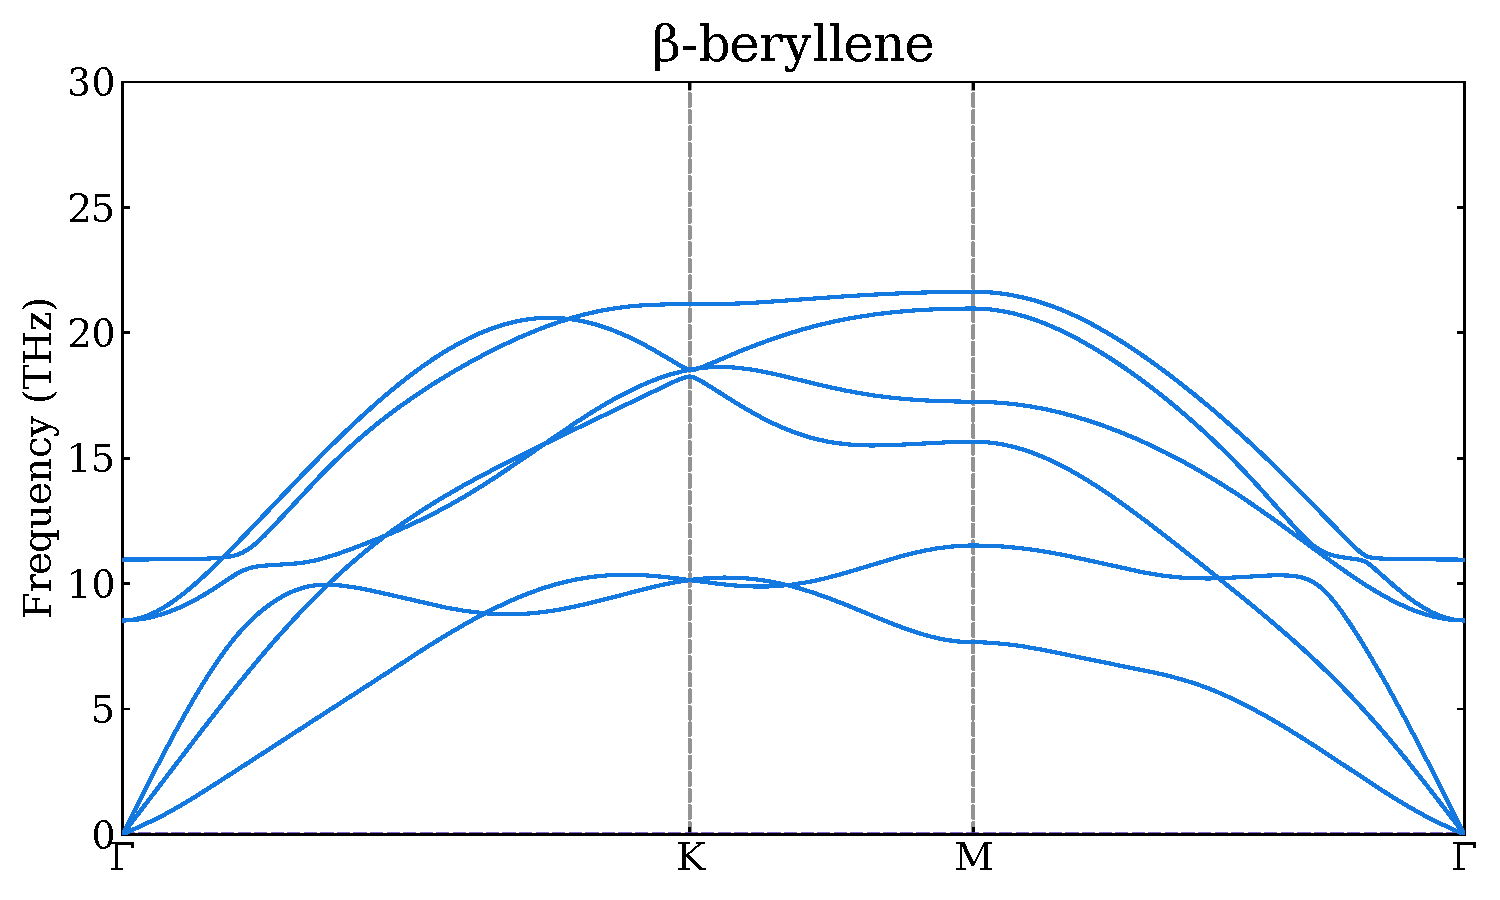
\includegraphics[width=0.40\linewidth]{figures_proj3/phonon/phonon_beta-beryllene_thesis.pdf}
\end{tabular}
\caption{Phonon-dispersion curves for bulk hcp beryllium, $\alpha$-beryllene, bulk bcc beryllium, and $\beta$-beryllene.
Imaginary frequencies are shown as negative values.}
\label{fig:proj3_phonon_dispersion}
\end{figure}

\begin{figure}[!htbp]
\centering
    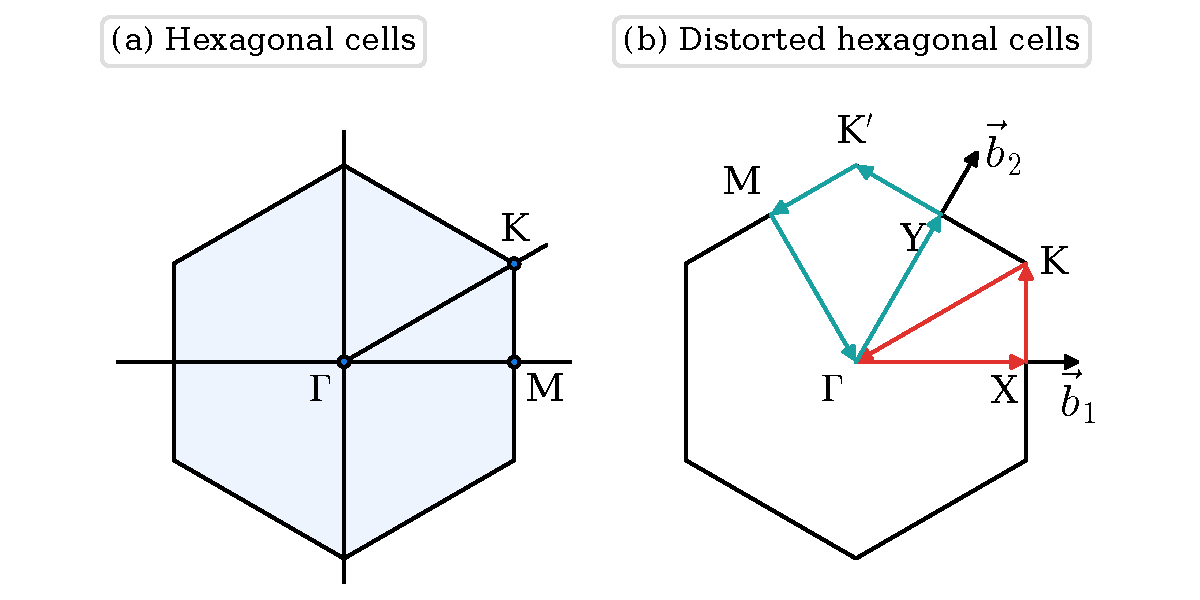
\includegraphics[width=0.80\linewidth]{figures_proj3/brillouin_zone_thesis.pdf}
\caption{Schematic Brillouin zones of the hexagonal and distorted hexagonal cells.
(a) Brillouin zone for the hexagonal unit cells of $\alpha$-beryllene, $\beta$-beryllene, and 2H-$\alpha$-beryllene.
(b) Brillouin zone for the distorted hexagonal cells of 1H-$\beta$-beryllene and 2H-$\beta$-beryllene,
with the path $\Gamma$--$\mathrm{X}$--$\mathrm{K}$--$\Gamma$--$\mathrm{Y}$--$\mathrm{K}'$--$\mathrm{M}$--$\Gamma$ used for their band structures and phonon dispersions.
$\vec{b}_{1}$ and $\vec{b}_{2}$ are the reciprocal lattice vectors of each relaxed cell,
and all coordinates are given in this basis.
$\mathrm{X}=\vec{b}_{1}/2$,
$\mathrm{Y}=\vec{b}_{2}/2$,
and $\mathrm{M}=(\vec{b}_{2}-\vec{b}_{1}\,)/2$,
which is equivalent to $(\vec{b}_{1}+\vec{b}_{2}\,)/2$,
are the time-reversal invariant momenta on the zone boundary.
$\mathrm{K}$ and $\mathrm{K}'=-\mathrm{K}+\vec{b}_{2}$ are the zone corners,
which are related by time reversal,
with $\mathrm{K}=(0.315,\,0.370)$ for 1H-$\beta$-beryllene and $(0.298,\,0.298)$ for 2H-$\beta$-beryllene.}
\label{fig:proj3_brillouin_zones}
\end{figure}

\begin{figure}[!htbp]
\centering
\begin{tabular}{@{}cc@{}}
% \begin{tabular}{cc}
    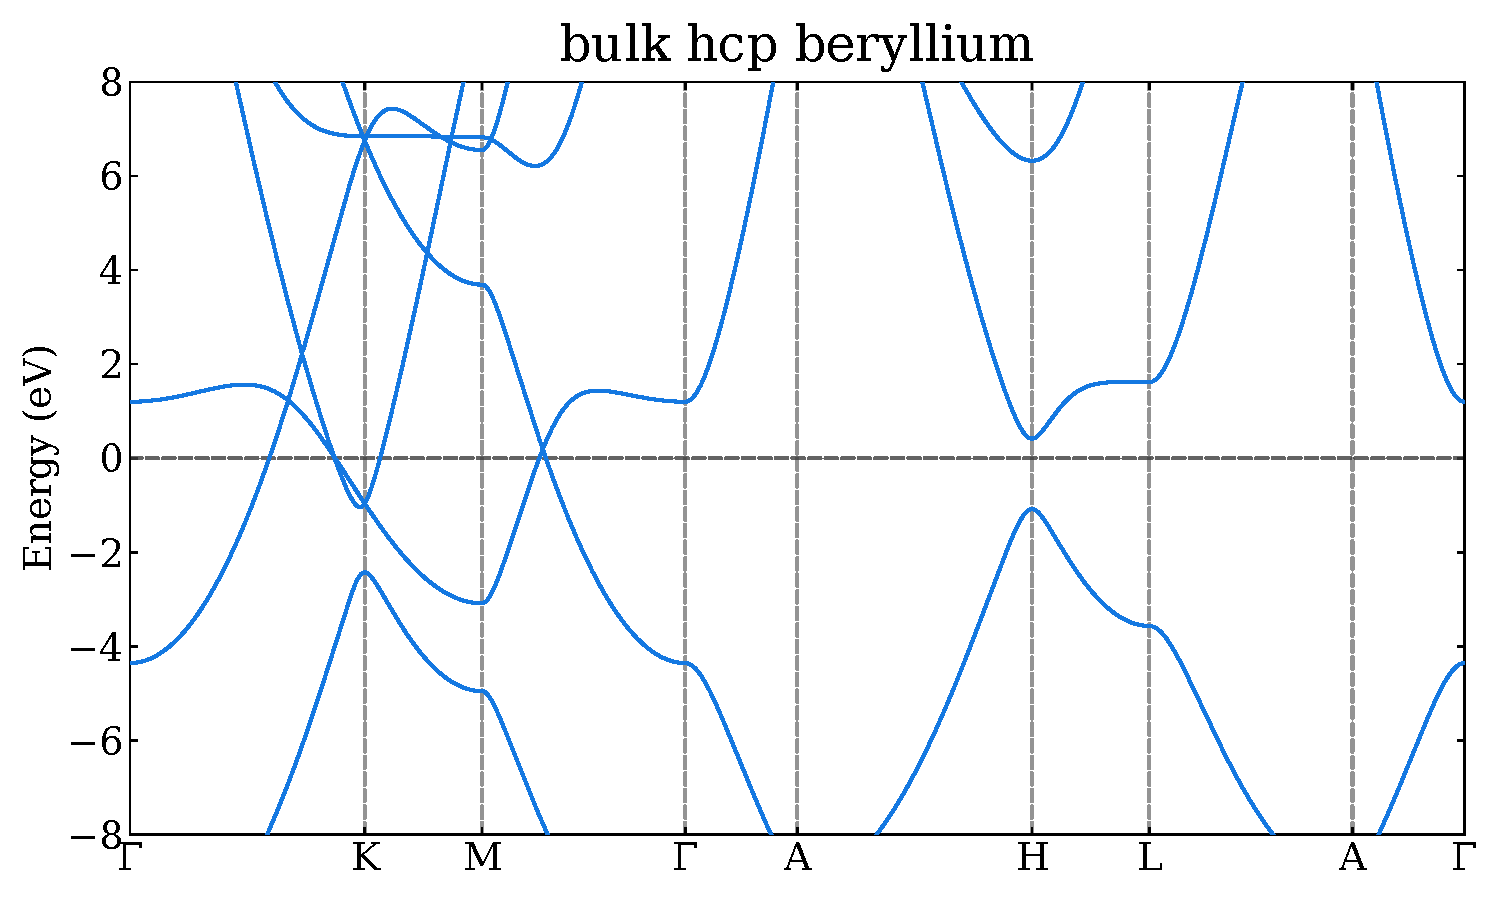
\includegraphics[width=0.40\linewidth]{figures_proj3/bands_hcp-beryllium_thesis.pdf}&
    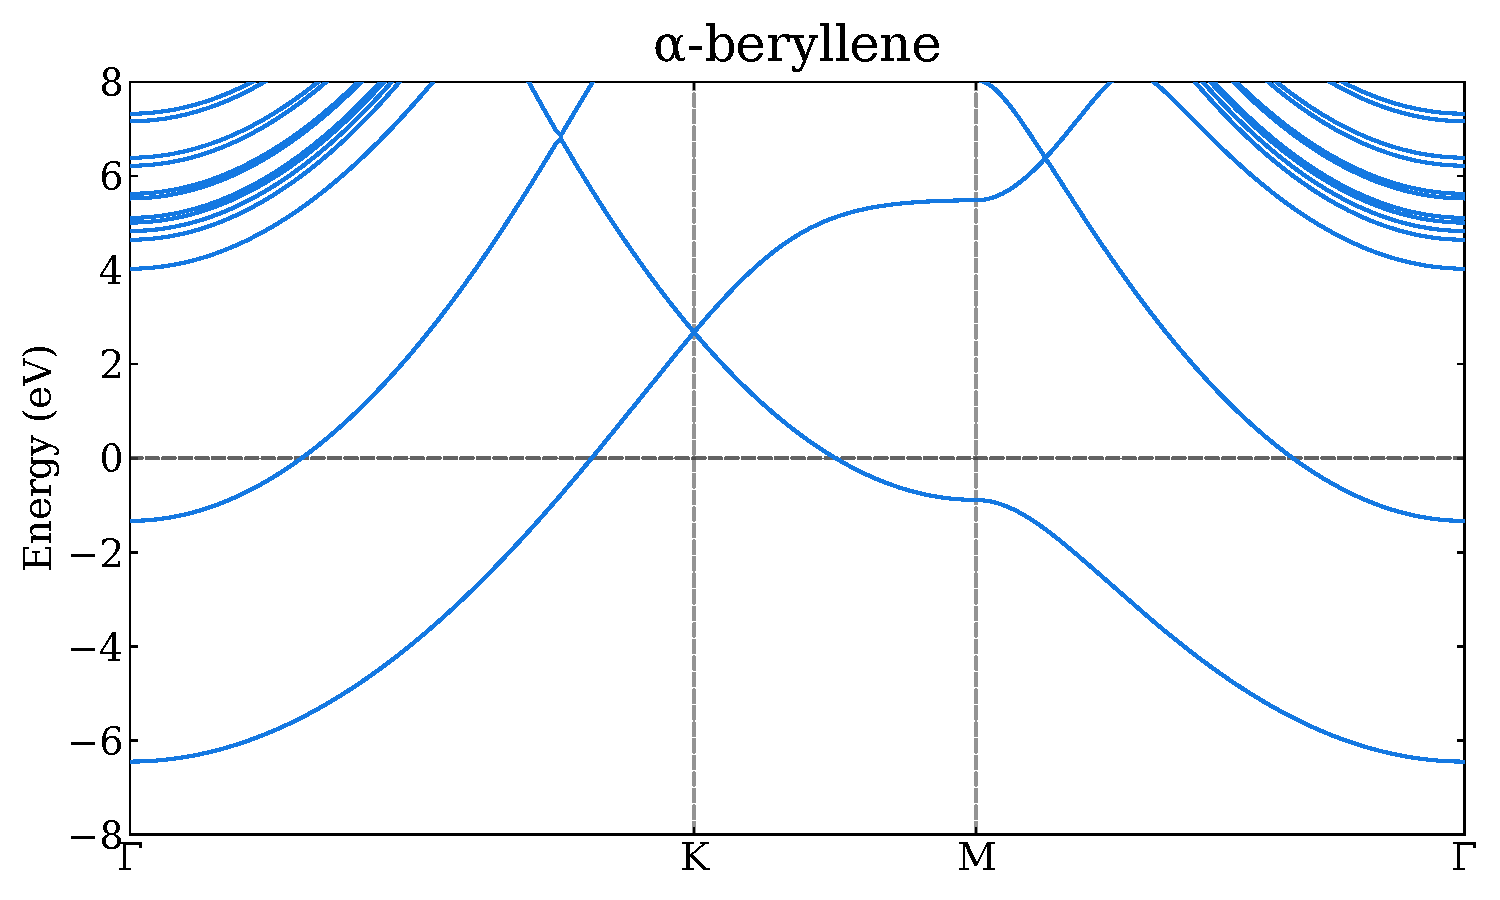
\includegraphics[width=0.40\linewidth]{figures_proj3/bands_alpha-beryllene_thesis.pdf}\\
    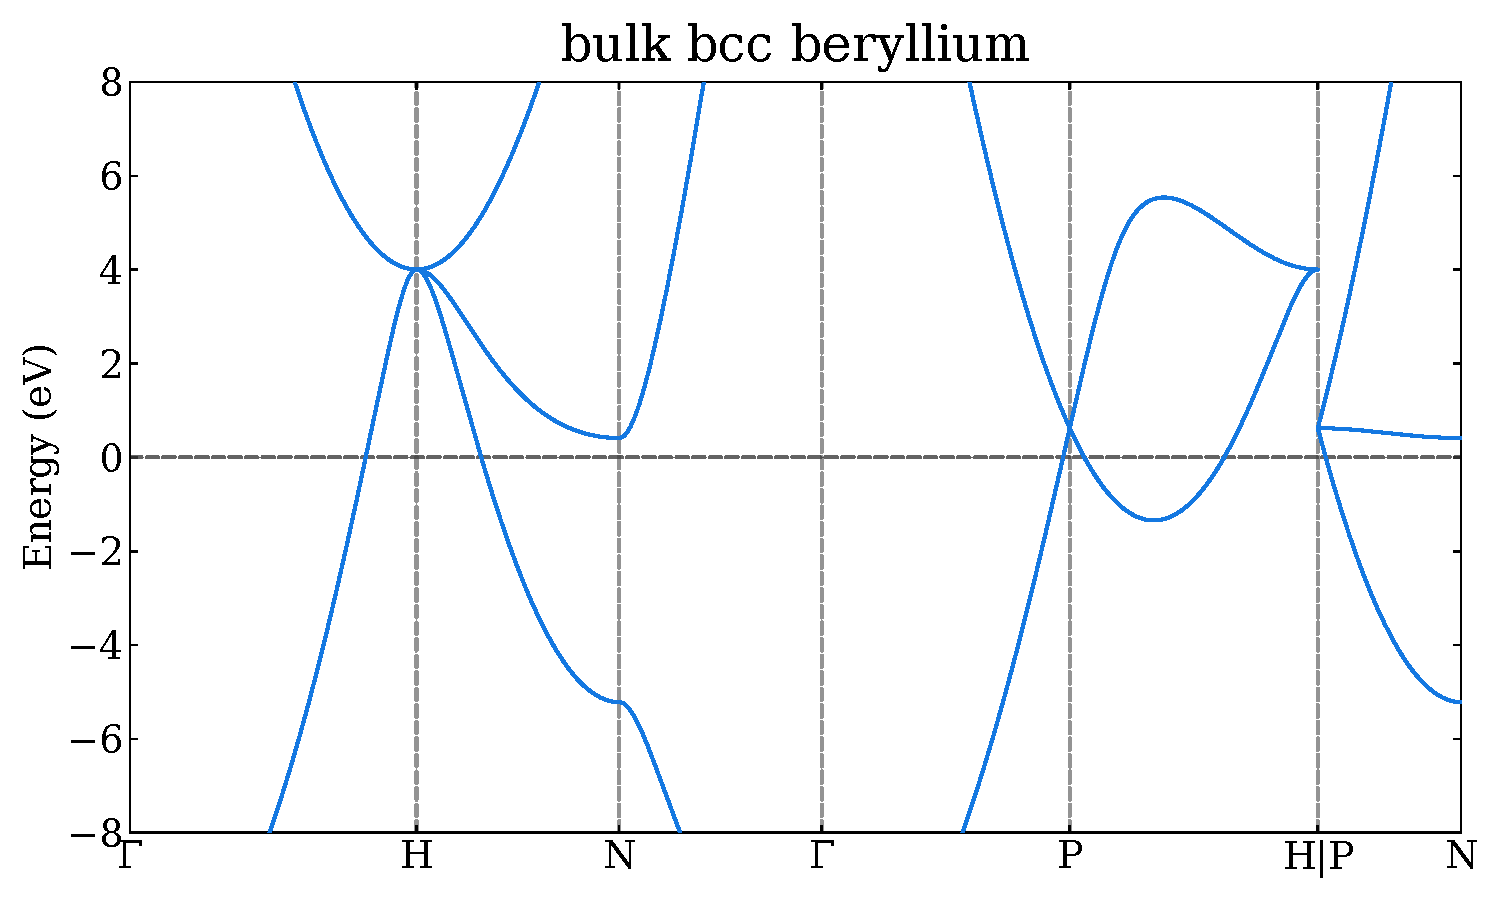
\includegraphics[width=0.40\linewidth]{figures_proj3/bands_bcc-beryllium_thesis.pdf}&
    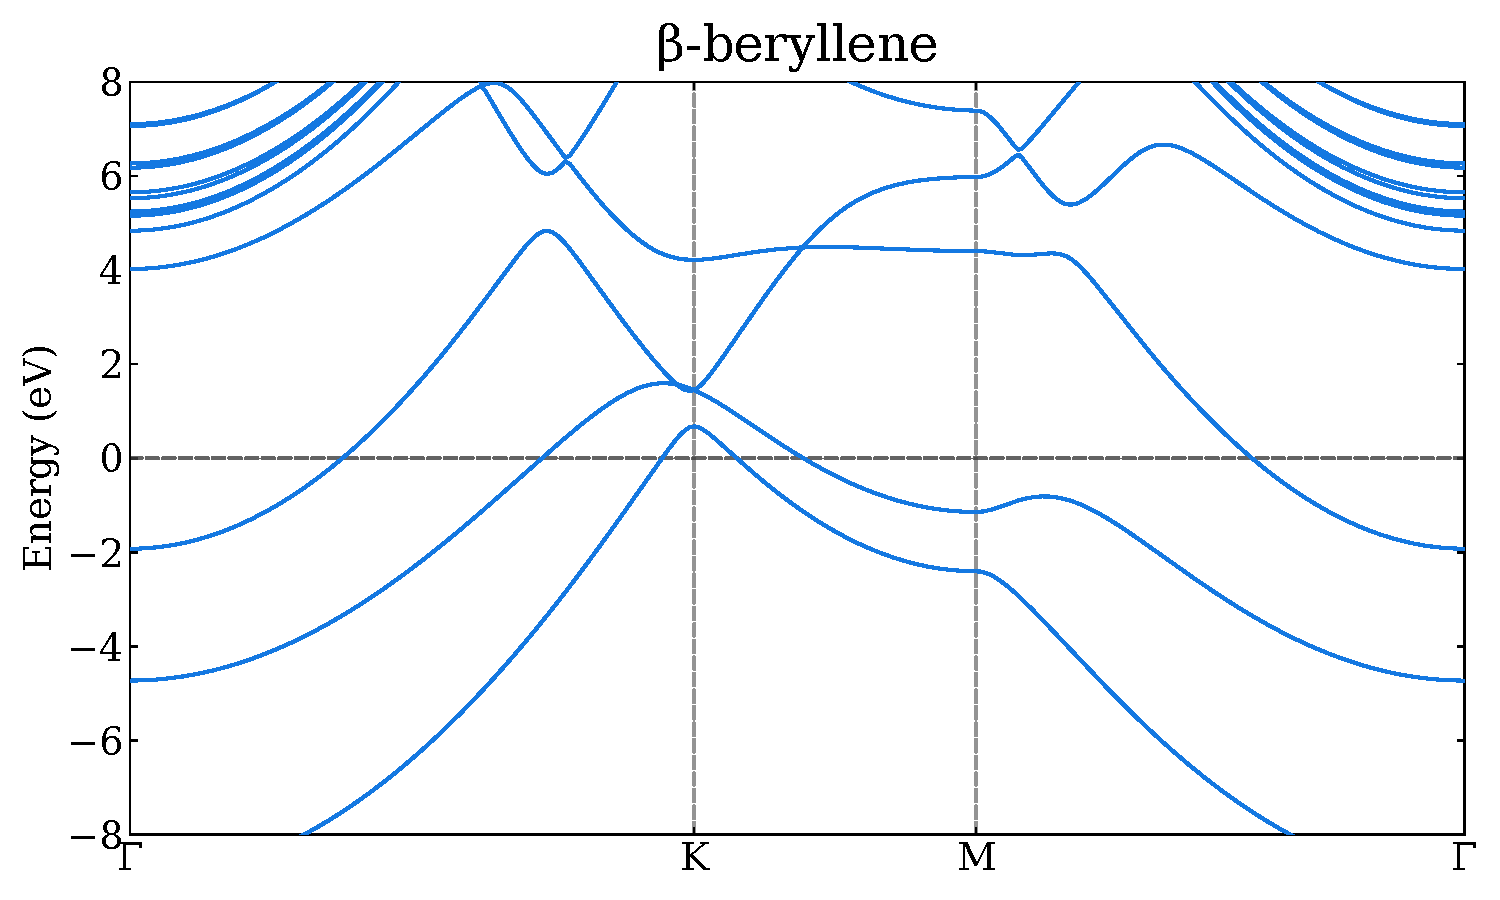
\includegraphics[width=0.40\linewidth]{figures_proj3/bands_beta-beryllene_thesis.pdf}
\end{tabular}
\caption{Band structures of bulk hcp beryllium, $\alpha$-beryllene, bulk bcc beryllium, and $\beta$-beryllene.}
\label{fig:proj3_band_structures}
\end{figure}

\FloatBarrier
\subsection*{Soft mode of 2H-$\beta$-beryllene}

The soft mode of 2H-$\beta$-beryllene occurs at $\vec{q}=(-0.4,0.4)$ in reciprocal-lattice coordinates along $\Gamma$--$\mathrm{M}$.
This wave vector is commensurate with the $5 \times 5$ phonon supercell.
For the frozen-phonon calculations, we use a smaller commensurate cell of 20 atoms with $\vec{A}_{1}=5\vec{a}_{1}$ and $\vec{A}_{2}=\vec{a}_{1}+\vec{a}_{2}$.
We scale the soft-mode eigenvector so that the largest atomic displacement is \qty{0.025}{\angstrom}, \qty{0.049}{\angstrom}, or \qty{0.098}{\angstrom}.
At each amplitude we calculate the energy with the atoms fixed.
For Gaussian smearing of \qty{0.02}{\electronvolt}, we use a $16 \times 97 \times 1$ k-point mesh.
For smearing of \qty{0.05}{\electronvolt} and \qty{0.10}{\electronvolt}, we use an $11 \times 65 \times 1$ mesh.

We fit the energy change to the quartic potential $E(Q)-E(0)=aQ^{2}+bQ^{4}$, with $Q$ the mass-weighted mode amplitude.
The curvature $2a$ at $Q=0$ determines the harmonic frequency.
For $a<0$ and $b>0$, the well depth is $a^{2}/(4b)$.
The fitted imaginary harmonic frequencies range from $1.0\mathrm{i}$ to $1.8\mathrm{i}$~\unit{\tera\hertz}, compared with $1.65\mathrm{i}$~\unit{\tera\hertz} from the phonon calculation.

We estimate the quantum fluctuations by solving the one-dimensional Schr\"odinger equation in the fitted potential.
We also obtain the self-consistent harmonic angular frequency $\Omega$ from $\Omega^{2}=2a+12b\langle Q^{2}\rangle$.
The harmonic variance is $\langle Q^{2}\rangle=\frac{\hbar}{2\Omega}\coth\!\left(\frac{\hbar\Omega}{2\kB T}\right)$ at temperature $T$.
Both estimates treat the soft mode independently of the other phonons.
Table~\ref{tab:proj3_soft_mode} compares the three smearing values.
In each case, the ground state lies approximately \qty{6}{\milli\electronvolt} above the potential minimum, far above the central barrier.
The first excitation energy corresponds to approximately \qty{4}{\tera\hertz}.
The ground-state root-mean-square amplitude is \qtyrange{0.35}{0.36}{\dalton\tothe{1/2}\angstrom}.
This exceeds the displacement of either well minimum from the origin, \qtyrange{0.14}{0.24}{\dalton\tothe{1/2}\angstrom}.
At a smearing of \qty{0.02}{\electronvolt}, the maximum fit residual of \qty{0.16}{\milli\electronvolt} is comparable to the fitted well depth.
The fit therefore resolves the depth poorly at this smearing.

\begin{table}[!htbp]
\centering
\rowcolors{2}{gray!15}{white}
\begin{adjustbox}{max width=1.0\linewidth,center}
\begin{tabular}{lccc}
\hline
\rowcolor{gray!25}
Gaussian smearing (eV) & 0.02 & 0.05 & 0.10 \\
supercell k-point mesh & $16 \times 97 \times 1$ & $11 \times 65 \times 1$ & $11 \times 65 \times 1$ \\
\hline
$\Delta E$ at \qty{0.025}{\angstrom} (meV) & $0.015$ & $-0.013$ & $-0.012$ \\
$\Delta E$ at \qty{0.049}{\angstrom} (meV) & $-0.007$ & $0.578$ & $0.495$ \\
$\Delta E$ at \qty{0.098}{\angstrom} (meV) & $10.029$ & $12.450$ & $11.932$ \\
fitted harmonic frequency (THz) & $1.75\mathrm{i}$ & $1.02\mathrm{i}$ & $1.13\mathrm{i}$ \\
double-well depth (meV) & $0.185$ & $0.021$ & $0.032$ \\
maximum fit residual (meV) & $0.158$ & $0.001$ & $0.018$ \\
\hline
ground state above the well bottom (meV) & $5.88$ & $6.31$ & $6.21$ \\
first excitation frequency (THz) & $3.77$ & $4.00$ & $3.95$ \\
self-consistent frequency at \qty{0}{\kelvin} (THz) & $4.03$ & $4.23$ & $4.18$ \\
self-consistent frequency at \qty{300}{\kelvin} (THz) & $5.54$ & $5.67$ & $5.63$ \\
\hline
\end{tabular}
\end{adjustbox}
\caption{Frozen-phonon energy changes and one-mode quantum estimates for the soft mode of 2H-$\beta$-beryllene.
Each column gives the results for one electronic smearing and k-point mesh.
The energy changes are relative to the undistorted 20-atom supercell.}
\label{tab:proj3_soft_mode}
\end{table}

We test for electronic nesting with the bare static susceptibility $\chi_0(\vec{q}\,)$ and the nesting function $\xi(\vec{q}\,)$ in figure~\ref{fig:proj3_nesting}.
Both quantities peak away from the soft-mode wave vector in the constant-matrix-element approximation.

\begin{figure}[!htbp]
\centering
    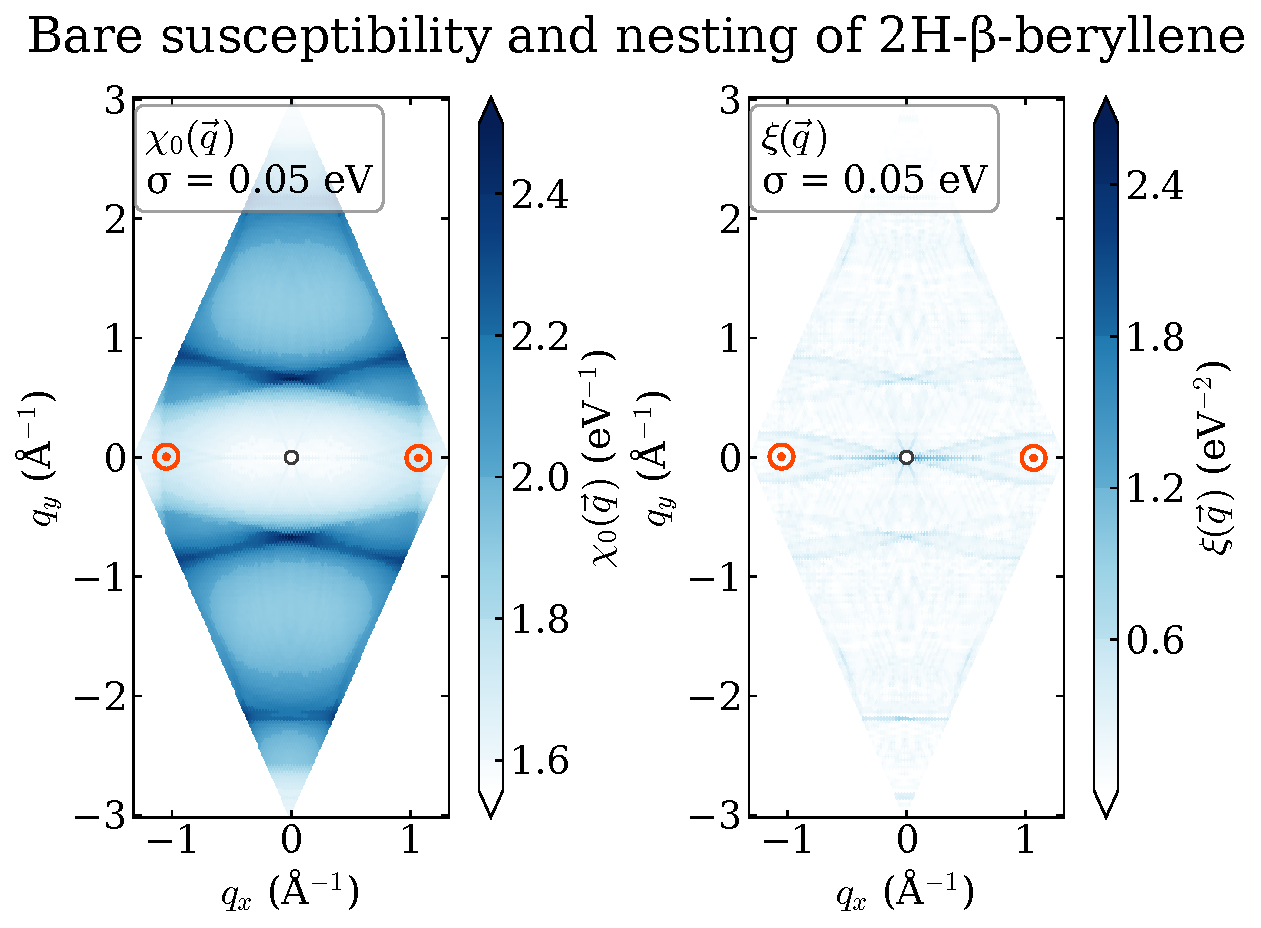
\includegraphics[width=0.80\linewidth]{figures_proj3/nesting_2H-beta-beryllene_thesis.pdf}
\caption{Bare static susceptibility $\chi_{0}(\vec{q}\,)$ (left) and nesting function $\xi(\vec{q}\,)$ (right) of 2H-$\beta$-beryllene,
calculated with constant matrix elements from the spin-orbit-coupled eigenvalues on the $105 \times 105$ mesh,
with Gaussian smearing of \qty{0.05}{\electronvolt}.
The bands with states within \qty{1}{\electronvolt} of the Fermi level are included.
The circled dots mark the soft-mode wave vector and its symmetry images,
and the open circle marks $\vec{q}=0$, whose value is excluded from the colour scale.
Among the 11024 non-zero wave vectors of the mesh,
the soft-mode wave vector ranks between 8723 and 8935 in $\chi_{0}$ and between 3806 and 8405 in $\xi$ for smearing between 0.02 and \qty{0.10}{\electronvolt}.}
\label{fig:proj3_nesting}
\end{figure}

\FloatBarrier
\subsection*{Hydrogenation energetics}

Table~\ref{tab:proj3_hydrogenation_energetics} shows the adsorption energies and free energies per hydrogen atom relative to \ce{H2}.
We use the harmonic phonons on a $40 \times 40$ q-point mesh and the molecular zero-point energy specified in section~\ref{3_methods}.
The zero-point correction raises the adsorption energies by \qtyrange{0.08}{0.09}{\electronvolt} per hydrogen atom.
At \qty{298.15}{\kelvin} and \qty{1}{\bar}, the thermal correction to the gas chemical potential is $H(T)-H(0)-TS=\qty{-0.316}{\electronvolt}$ per \ce{H2} molecule.

For ideal-gas \ce{H2}, the adsorption free energy per H vanishes at $p_{\mathrm{eq}}=p^{\circ}\exp\!\left(\frac{2\Delta G}{\kB T}\right)$.
Here, $\Delta G$ refers to the adsorption free energy per H at the standard pressure $p^{\circ}=\qty{1}{\bar}$.
The factor of two converts the adsorption free energy per H to the corresponding value per \ce{H2} molecule.
The pressure for 1H-$\beta$-beryllene is a formal extrapolation of the ideal-gas relation.

For 2H-$\beta$-beryllene, we omit the imaginary modes, whose wave vectors cover approximately \qty{1.1}{\percent} of the Brillouin zone.
Its free energy and equilibrium pressure are therefore conditional on this harmonic treatment.

\begin{table}[!htbp]
\centering
\rowcolors{2}{gray!15}{white}
\begin{tabular}{ccccc}
\hline
\rowcolor{gray!25}
structure
& $E_{\mathrm{ad}}$ (eV)
& $E_{\mathrm{ad}}+\Delta E_{\mathrm{ZPE}}$ (eV)
& $\Delta G$ (eV)
& $p_{\mathrm{eq}}$ (bar) \\
\hline
2H-$\alpha$-beryllene & $-0.331$ & $-0.243$ & $-0.084$ & $1.4\times10^{-3}$ \\
1H-$\beta$-beryllene & $-0.072$ & $0.012$ & $0.166$ & $4.0\times10^{5}$ \\
2H-$\beta$-beryllene & $-0.173$ & $-0.090$ & $0.058$ & $93$ \\
\hline
\end{tabular}
\caption{Electronic adsorption energy $E_{\mathrm{ad}}$ from equation~\eqref{eq:proj3_hydrogen_adsorption_energy}, zero-point-corrected adsorption energy, and adsorption free energy $\Delta G$, all per hydrogen atom.
At \qty{298.15}{\kelvin}, $\Delta G$ refers to \qty{1}{\bar} of \ce{H2}, and $p_{\mathrm{eq}}$ is the pressure at which the adsorption free energy vanishes.}
\label{tab:proj3_hydrogenation_energetics}
\end{table}

Table~\ref{tab:proj3_beh2_polymorphs} compares the relaxed energies of four \ce{BeH2} monolayers.
We relax all four structures with the same settings and assign space groups with a tolerance of \qty{1e-3}{\angstrom}.
With aligned hollow sites for hydrogen on the two sides, the layer relaxes to a $Cmmm$ structure.
Its energy is \qty{0.74}{\electronvolt} per formula unit above that of the staggered structure.
The comparison concerns relaxed energies, with the dynamical stability of the puckered square layer left open.

\begin{table}[!htbp]
\centering
\rowcolors{2}{gray!15}{white}
\begin{adjustbox}{max width=1.0\linewidth,center}
\begin{tabular}{cccc}
\hline
\rowcolor{gray!25}
structure & space group & Be-H coordination & $\Delta E$ (meV per \ce{BeH2}) \\
\hline
2H-$\alpha$-beryllene, staggered hollows & $P\bar{3}m1$ & 6 H at \qty{1.599}{\angstrom} & $0$ \\
2H-$\alpha$-beryllene, aligned hollows & $Cmmm$ & 4 H at \qty{1.488}{\angstrom} & $740.6$ \\
puckered square layer & $P\bar{4}m2$ & 4 H at \qty{1.468}{\angstrom} & $-38.2$ \\
planar square layer & $P4/mmm$ & 4 H at \qty{1.479}{\angstrom} & $1233.1$ \\
\hline
\end{tabular}
\end{adjustbox}
\caption{Space groups,
coordination of beryllium by hydrogen,
and relaxed total energies per formula unit relative to 2H-$\alpha$-beryllene for the \ce{BeH2} monolayers considered.}
\label{tab:proj3_beh2_polymorphs}
\end{table}

\FloatBarrier
\subsection*{Topological screening}

Figures~\ref{fig:proj3_direct_gap_pristine} and~\ref{fig:proj3_direct_gap_hydrogenated} map the direct gap $E_{N+1}-E_{N}$ above the lowest $N$ spinor bands.
We reconstruct the full $105 \times 105$ mesh from its irreducible part using the symmetries of each structure.
To refine the minima, we calculate spinor eigenvalues on denser local meshes at fixed self-consistent charge density.

The smallest sampled gaps in the pristine structures are approximately \qty{1}{\milli\electronvolt}.
We therefore refine each local minimum on successively smaller $9 \times 9$ patches, as shown in figure~\ref{fig:proj3_gap_zoom}.
After four refinements, the minimum for $\alpha$-beryllene lies within $5\times10^{-6}$ of $\mathrm{K}$ in each fractional reciprocal coordinate.
The minimum for $\beta$-beryllene stays at $\mathrm{K}$, and that of the cubic trilayer stays on $\Gamma$--$\mathrm{M}$ through five levels.
At each level, we subtract the largest sampled gap slope times the sampling radius from the smallest sampled gap.
On the finest patches this gives \qty{1.07}{\milli\electronvolt} for $\alpha$-beryllene, \qty{0.65}{\milli\electronvolt} for $\beta$-beryllene, and \qty{0.71}{\milli\electronvolt} for the cubic trilayer.
These local estimates depend on the sampled slopes and leave open the possibility of a gap closing between sampled points.
Convergence with respect to the plane-wave cutoff and the self-consistent k-point mesh also remains to be tested directly for these gaps.

The smallest sampled direct gap of the hydrogen-functionalized structures is \qty{0.177}{\electronvolt}.
Figure~\ref{fig:proj3_wcc} shows the Wannier charge centres for the lowest four and lowest six bands of 1H-$\beta$-beryllene.
The Wilson-loop analysis over half of the Brillouin zone gives $\nu=0$ for each of these two subspaces.

Table~\ref{tab:proj3_hse_parity} compares parities from HSE06 without spin-orbit coupling and from PBE with spin-orbit coupling.
At each time-reversal invariant momentum, the number of odd states among the lowest $N/2$ spinless HSE06 bands matches the number of odd PBE Kramers pairs.
The matching counts give the same parity products at these four momenta.
For 2H-$\beta$-beryllene, the scalar-relativistic gap at $\mathrm{M}$ is \qty{0.171}{\electronvolt} with HSE06 and \qty{0.178}{\electronvolt} with PBE in the same cell.

We test the time-reversal assumption against the magnetization density and band energies.
The converged spin-orbit-coupled states have a maximum magnetization density below $3\times10^{-7}~\mu_{\mathrm{B}}\,\text{\AA}^{-3}$.
The Kramers splittings at time-reversal invariant momenta are at most \qty{3.8e-6}{\electronvolt}.
For 1H-$\beta$-beryllene, the eigenvalues at $\vec{k}$ and $-\vec{k}$ agree within \qty{4.0e-7}{\electronvolt} across all 5512 pairs on the mesh.
We start collinear spin-polarized calculations from ferromagnetic and antiferromagnetic configurations, with additional inversion-odd configurations for trilayer cubic beryllene.
All 11 calculations converge to site moments below $10^{-3}~\mu_{\mathrm{B}}$.

\begin{table}[!htbp]
\centering
\rowcolors{2}{gray!15}{white}
\begin{adjustbox}{max width=1.0\linewidth,center}
\begin{tabular}{ccccc}
\hline
\rowcolor{gray!25}
structure
& $N$
& odd pairs at $\Gamma$, $\mathrm{X}$, $\mathrm{Y}$, $\mathrm{M}$
& $\nu$
& smallest gap (eV), HSE06 / PBE \\
\hline
$\alpha$-beryllene & 2 & 0, 1, 1, 1 & 1 & $\Gamma$: 6.209 / 5.169 \\
$\beta$-beryllene & 4 & 1, 1, 1, 1 & 0 & $\Gamma$: 3.471 / 2.795 \\
trilayer cubic beryllene & 6 & 1, 1, 1, 2 & 1 & $\mathrm{M}$: even-parity doublet \\
2H-$\alpha$-beryllene & 4 & 1, 1, 1, 1 & 0 & $\mathrm{X}$: 6.847 / 5.644 \\
2H-$\beta$-beryllene & 6 & 1, 1, 2, 2 & 0 & $\mathrm{M}$: 0.171 / 0.178 \\
\hline
\end{tabular}
\end{adjustbox}
\caption{Numbers of odd-parity Kramers pairs among the lowest $N$ bands at the time-reversal invariant momenta,
$\mathbb{Z}_2$ indices,
and smallest gaps $E_{N+1}-E_{N}$ at the time-reversal invariant momenta.
The counts are the same for the lowest $N/2$ spinless HSE06 states and the lowest $N/2$ PBE Kramers pairs.
The listed $\mathbb{Z}_2$ indices are conditional PBE results with spin-orbit coupling.
The HSE06 and PBE gaps are calculated in the same \qty{20}{\angstrom} cell without spin-orbit coupling.
For trilayer cubic beryllene,
the boundary of the lowest six bands at $\mathrm{M}$ lies within an orbital doublet of even parity,
which is split only by spin-orbit coupling.}
\label{tab:proj3_hse_parity}
\end{table}

\begin{figure}[!htbp]
\centering
    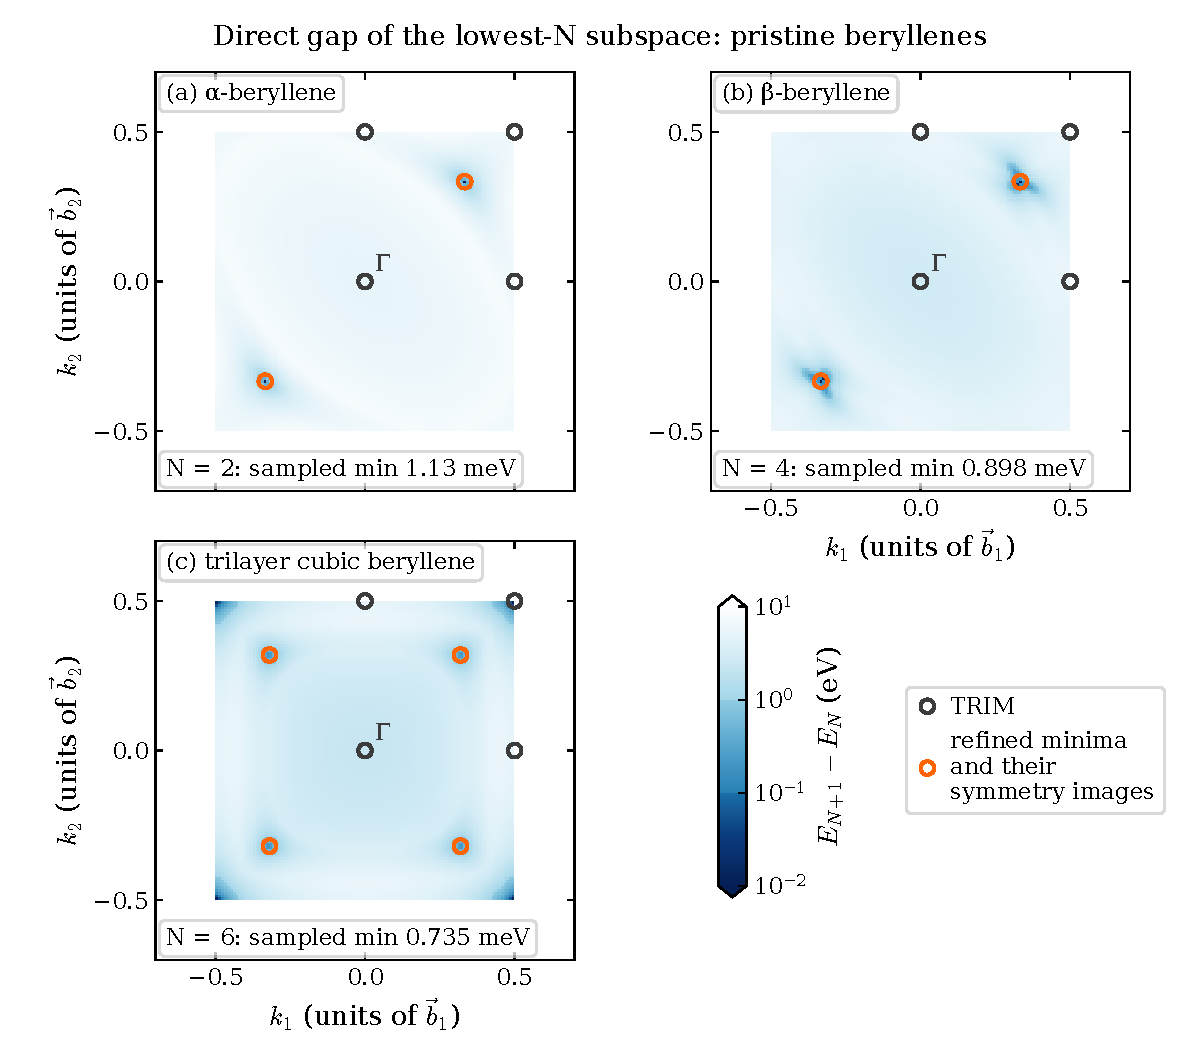
\includegraphics[width=0.80\linewidth]{figures_proj3/topology_direct-gap_pristine_thesis.pdf}
\caption{Direct gap $E_{N+1}-E_{N}$ of the lowest-$N$ subspace over the Brillouin zone for (a) $\alpha$-beryllene,
(b) $\beta$-beryllene,
and (c) trilayer cubic beryllene,
on a logarithmic scale.
The time-reversal invariant momenta,
the refined minima,
and their symmetry images are marked.}
\label{fig:proj3_direct_gap_pristine}
\end{figure}

\begin{figure}[!htbp]
\centering
    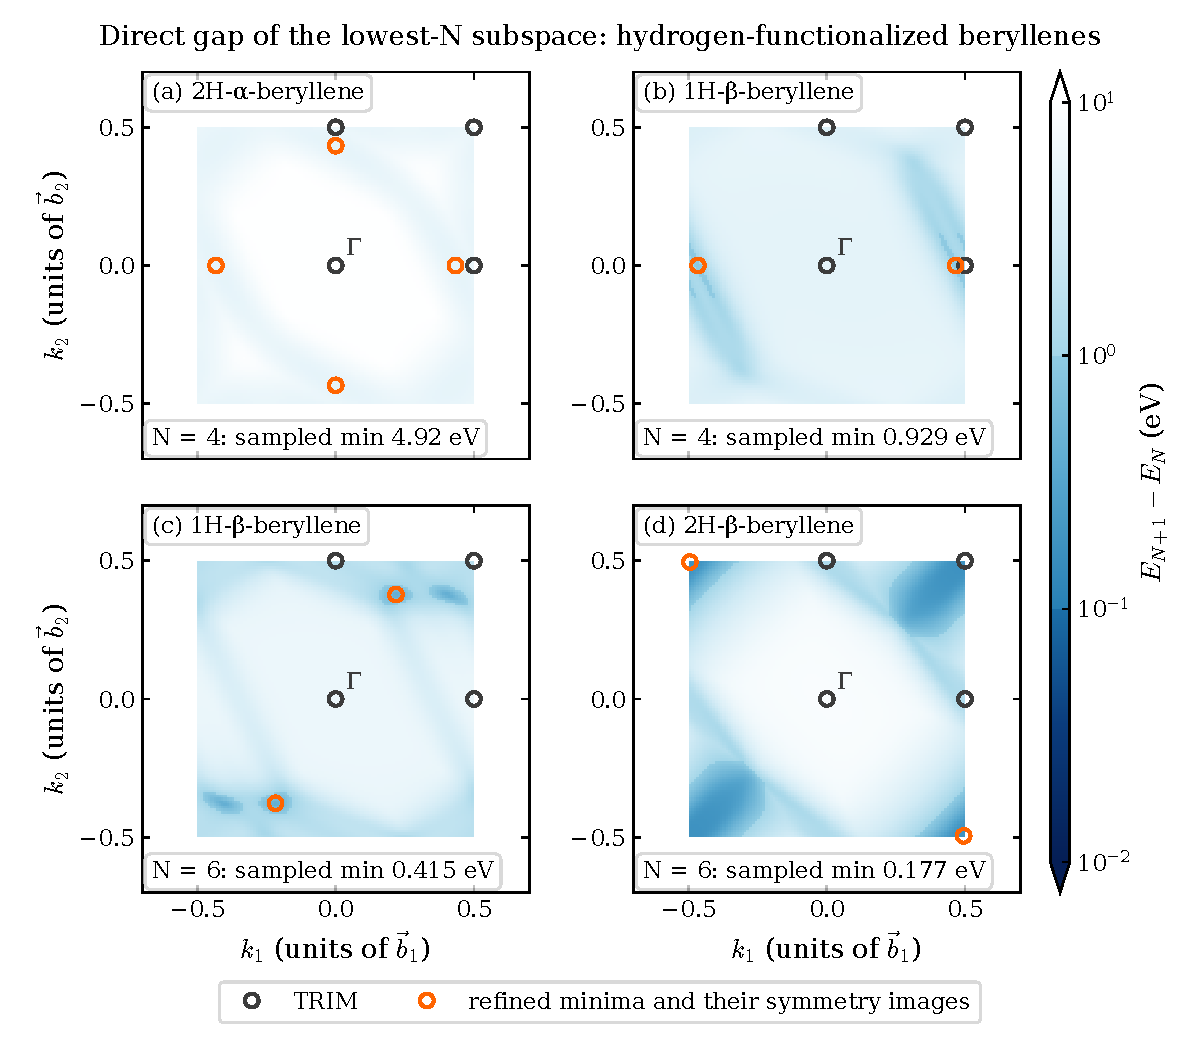
\includegraphics[width=0.80\linewidth]{figures_proj3/topology_direct-gap_hydrogenated_thesis.pdf}
\caption{Direct gap $E_{N+1}-E_{N}$ of the lowest-$N$ subspace over the Brillouin zone for (a) 2H-$\alpha$-beryllene,
(b, c) 1H-$\beta$-beryllene with $N=4$ and $N=6$,
and (d) 2H-$\beta$-beryllene,
shown as in figure~\ref{fig:proj3_direct_gap_pristine}.}
\label{fig:proj3_direct_gap_hydrogenated}
\end{figure}

\begin{figure}[!htbp]
\centering
    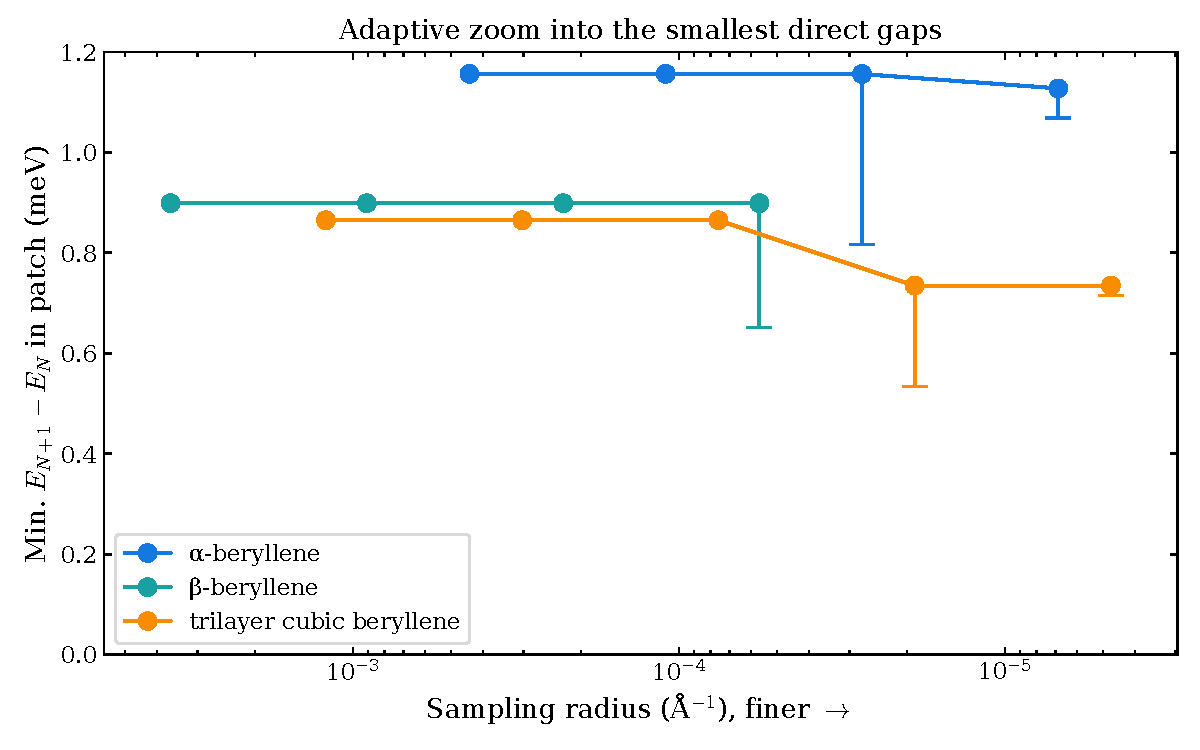
\includegraphics[width=0.80\linewidth]{figures_proj3/topology_gap-zoom_thesis.pdf}
\caption{Minimum direct gap in each refinement patch as a function of the sampling radius for $\alpha$-beryllene,
$\beta$-beryllene,
and trilayer cubic beryllene.
Where the local estimate from the sampled gap slopes is positive, a bar extends down from the sampled minimum to that estimate.}
\label{fig:proj3_gap_zoom}
\end{figure}

\begin{figure}[!htbp]
\centering
    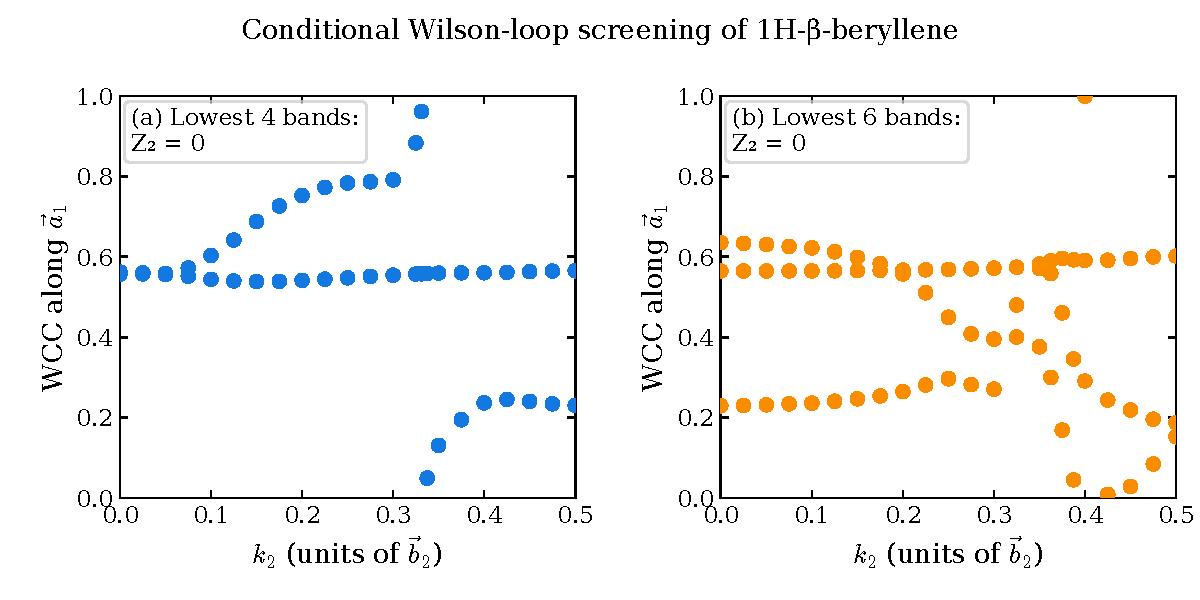
\includegraphics[width=0.80\linewidth]{figures_proj3/topology_wcc_1H-beta-beryllene_thesis.pdf}
\caption{Wannier charge centres of 1H-$\beta$-beryllene along $\vec{a}_{1}$ as functions of $k_{2}$ over half of the Brillouin zone,
for (a) the lowest four bands and (b) the lowest six bands.}
\label{fig:proj3_wcc}
\end{figure}

\FloatBarrier
\subsection*{Structures for the \texttt{Quantum ESPRESSO} calculations}

Table~\ref{tab:proj3_qe_structures} lists the PBE geometries used to cross-check the topology in \texttt{Quantum ESPRESSO}.
The phonon and electron-phonon calculations for 2H-$\beta$-beryllene use the PBE+D3 geometry in the last row.
With D3 included, the residual forces on this geometry are below \qty{0.03}{\electronvolt\per\angstrom}.

\begin{table}[!htbp]
\centering
\rowcolors{2}{gray!15}{white}
\begin{adjustbox}{max width=1.0\linewidth,center}
\begin{tabular}{ccccccc}
\hline
\rowcolor{gray!25}
system
& cell content
& $a$
& $b$
& angle
& thickness
& electronic nature \\
\hline
trilayer cubic beryllene
& \ce{Be3} & 2.18 & 2.18 & $90.00^{\circ}$ & 3.04 & metallic \\
2H-$\alpha$-beryllene
& \ce{BeH2} & 2.32 & 2.32 & $120.00^{\circ}$ & 1.74 & semiconductor \\
2H-$\beta$-beryllene
& \ce{Be2H2} & 2.62 & 2.62 & $133.12^{\circ}$ & 3.78 & metallic \\
1H-$\beta$-beryllene
& \ce{Be2H} & 2.32 & 2.11 & $117.01^{\circ}$ & 2.85 & metallic \\
\hline
2H-$\beta$-beryllene, PBE+D3
& \ce{Be2H2} & 2.53 & 2.53 & $131.88^{\circ}$ & 3.79 & metallic \\
\hline
\end{tabular}
\end{adjustbox}
\caption{Cell content,
lattice constants $a$ and $b$,
angle between the in-plane lattice vectors, thickness, and electronic character of the relaxed structures.
Thickness denotes the separation of the outermost atomic centres along the surface normal.
The lattice constants and thickness are in \unit{\angstrom}.
The last row gives the PBE+D3 geometry for the phonon and electron-phonon calculations of 2H-$\beta$-beryllene.}
\label{tab:proj3_qe_structures}
\end{table}

\FloatBarrier
\subsection*{Phonon and electron-phonon calculations}

On the $12 \times 12 \times 1$ q-point mesh, the density functional perturbation theory calculations give imaginary frequencies only at $\Gamma$.
The lowest values there are $0.14\mathrm{i}$, $0.24\mathrm{i}$, and $0.20\mathrm{i}$~\unit{\tera\hertz} for trilayer cubic beryllene, 2H-$\beta$-beryllene, and 1H-$\beta$-beryllene, respectively.
For these three structures, we interpolate with 12, 10, and 9 Wannier functions, respectively.
The upper edges of their frozen windows lie \qtyrange{3.0}{3.6}{\electronvolt} above the Fermi level.

Table~\ref{tab:proj3_epw_threshold} and figure~\ref{fig:proj3_a2f} compare the electron-phonon results for different meshes and lower phonon frequency thresholds.
For trilayer cubic beryllene and 2H-$\beta$-beryllene, frequencies from \qty{5}{\per\centi\metre} to \qty{40}{\per\centi\metre} account for approximately half of $\lambda$ on the $40 \times 40 \times 1$ fine meshes.
Integrating these same spectral functions above \qty{40}{\per\centi\metre} gives $\lambda=0.44$ for the trilayer and $\lambda=1.50$ for 2H-$\beta$-beryllene.
The corresponding results on the $80 \times 80 \times 1$ meshes are 0.46 and 1.40.
This comparison tests the mesh sensitivity of the contribution above the higher threshold.
For 1H-$\beta$-beryllene, both fine meshes include frequencies above \qty{5}{\per\centi\metre} and give similar couplings.

\begin{table}[!htbp]
\centering
\rowcolors{2}{gray!15}{white}
\begin{adjustbox}{max width=1.0\linewidth,center}
\begin{tabular}{cccccc}
\hline
\rowcolor{gray!25}
structure
& fine meshes
& threshold (\unit{\per\centi\metre})
& $\lambda$
& $\hbar\omega_\mathrm{log}$ (meV)
& $T_\mathrm{c}^{\mathrm{AD}}$ (K) \\
\hline
trilayer cubic beryllene & $40 \times 40 \times 1$ & 5 & 1.00 & 4.0 & 2.8 \\
trilayer cubic beryllene & $80 \times 80 \times 1$ & 40 & 0.46 & 36.0 & 2.0 \\
2H-$\beta$-beryllene & $40 \times 40 \times 1$ & 5 & 3.06 & 7.5 & 15.1 \\
2H-$\beta$-beryllene & $80 \times 80 \times 1$ & 40 & 1.40 & 19.5 & 21.9 \\
1H-$\beta$-beryllene & $40 \times 40 \times 1$ & 5 & 0.60 & 41.0 & 7.8 \\
1H-$\beta$-beryllene & $80 \times 80 \times 1$ & 5 & 0.61 & 40.7 & 8.1 \\
\hline
\end{tabular}
\end{adjustbox}
\caption{Electron-phonon coupling strength $\lambda$,
logarithmic average phonon energy $\hbar\omega_\mathrm{log}$,
and Allen--Dynes transition temperature $T_\mathrm{c}^{\mathrm{AD}}$ for $\mu^*=0.13$,
calculated with different fine meshes and lower phonon frequency thresholds.}
\label{tab:proj3_epw_threshold}
\end{table}

\begin{figure}[!htbp]
\centering
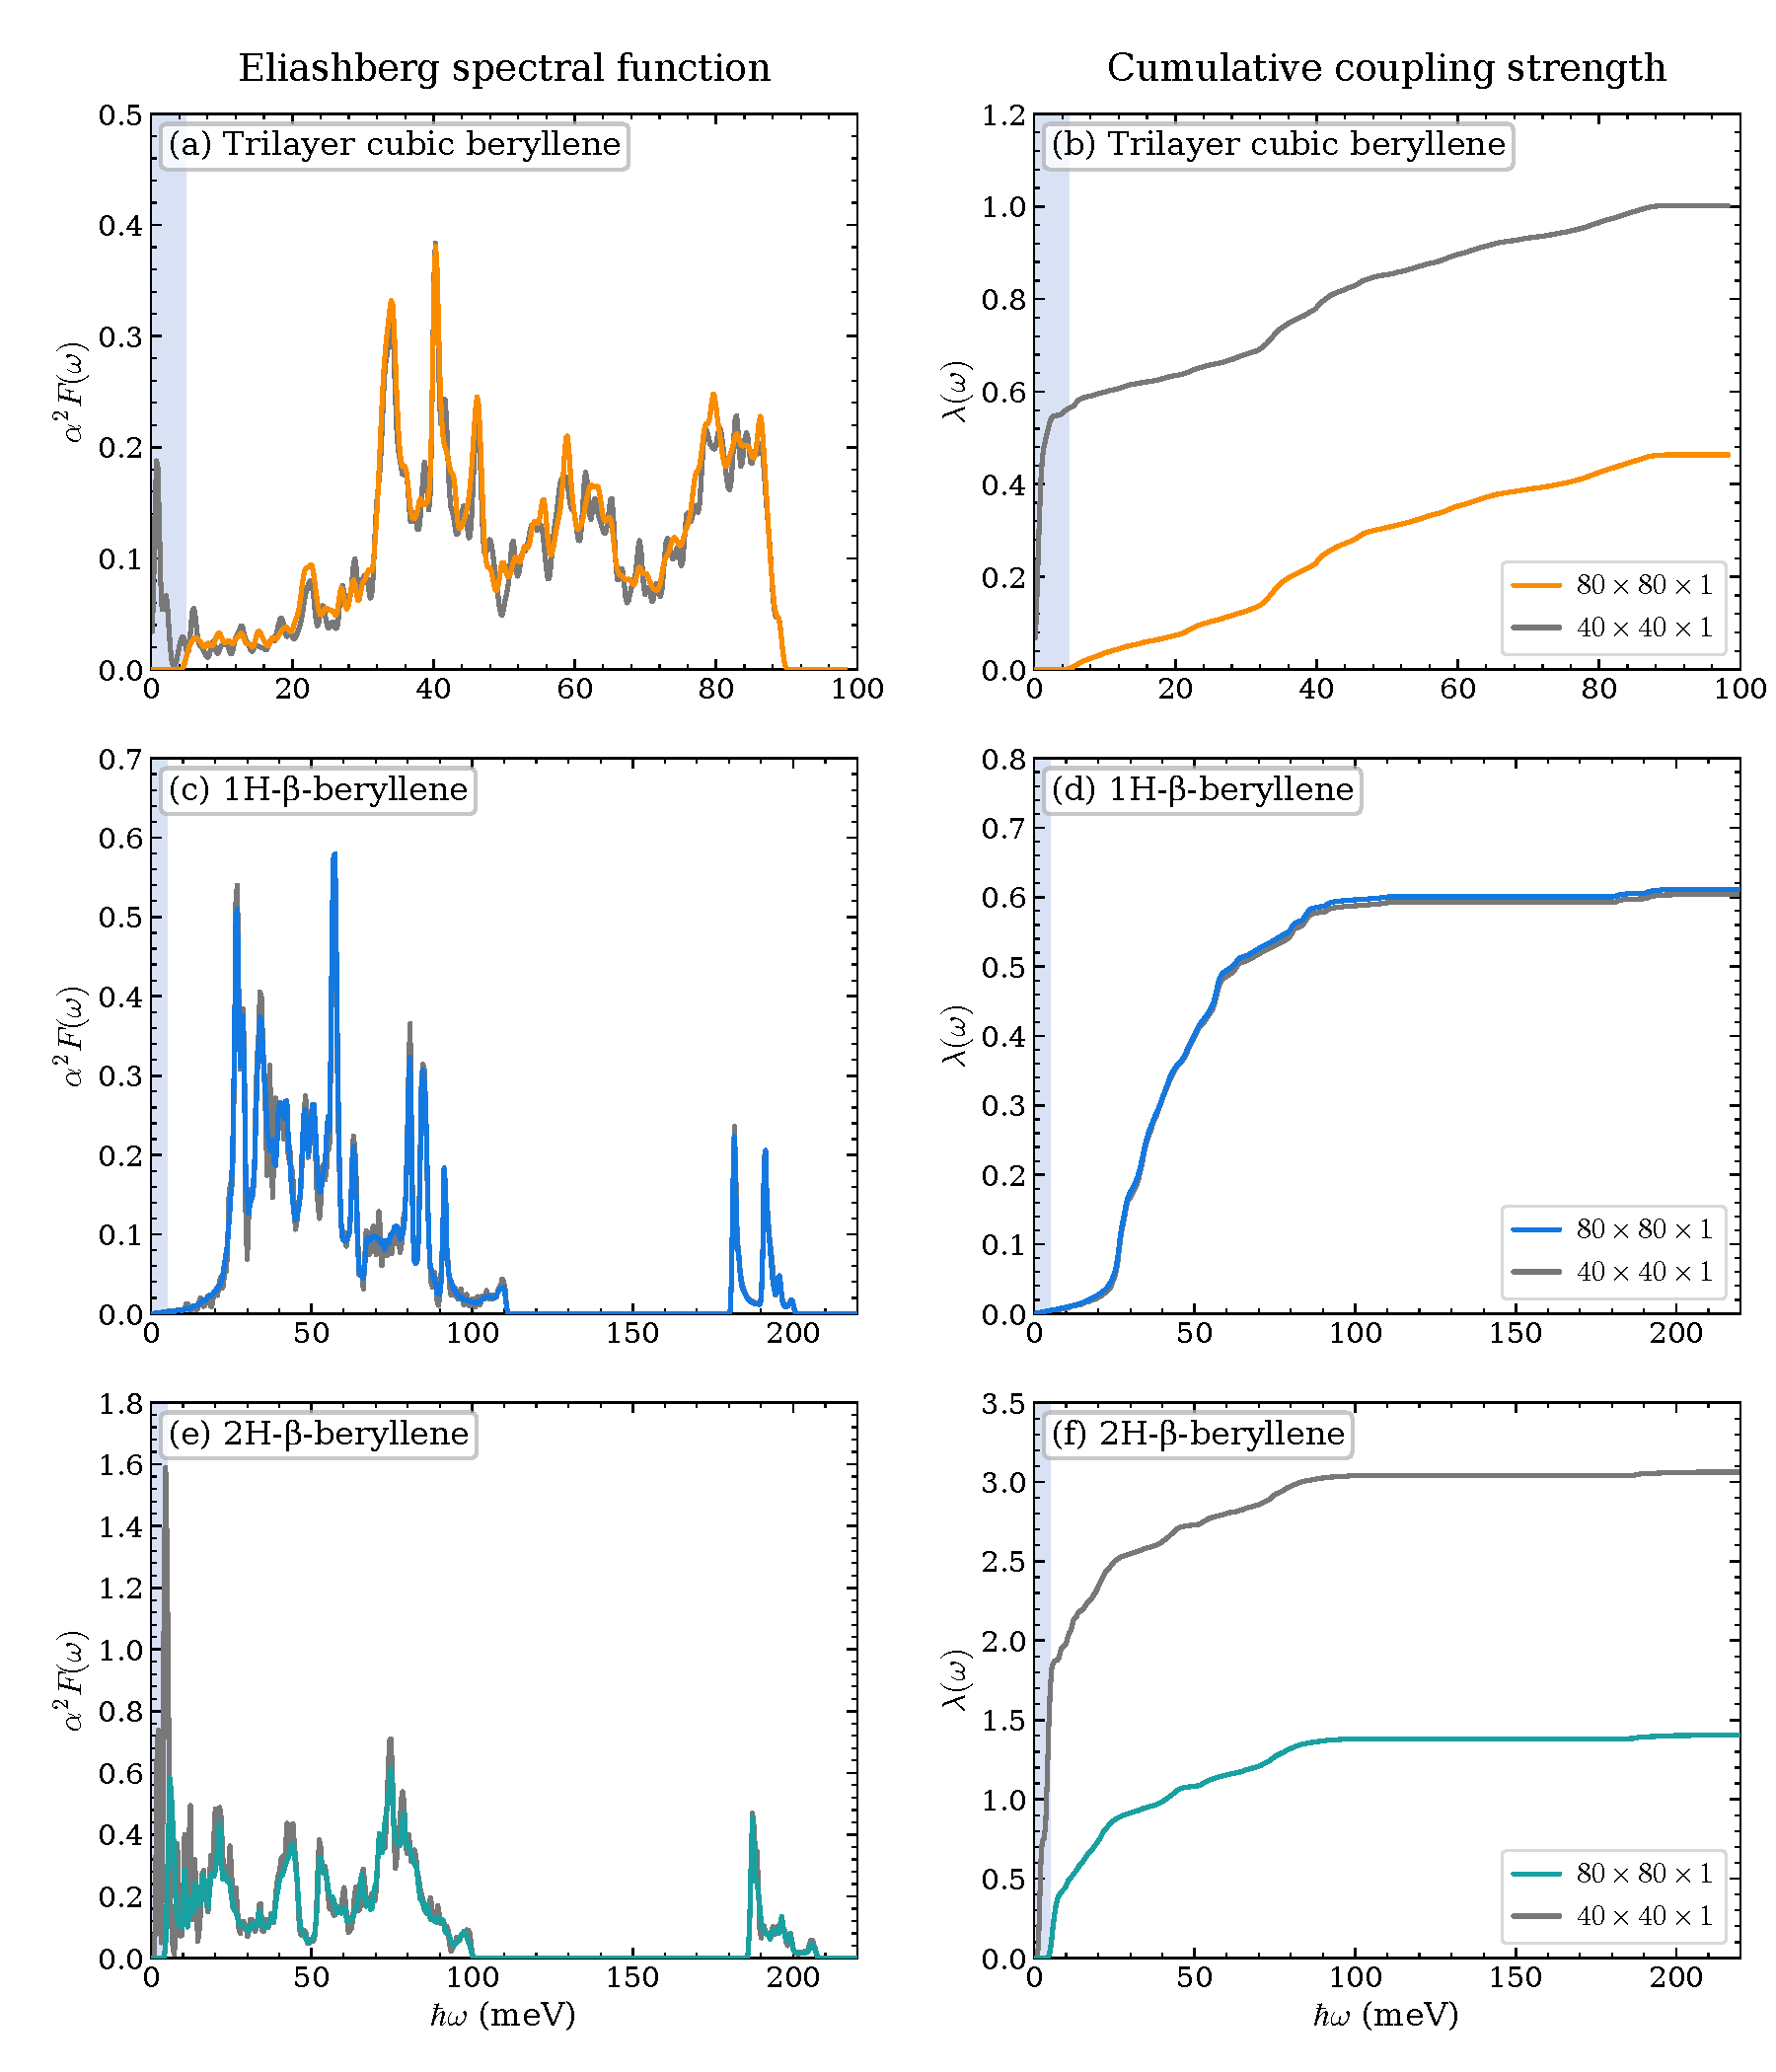
\includegraphics[width=0.80\linewidth]{figures_proj3/superconductivity/superconductivity_a2f.pdf}
\caption{Eliashberg spectral function $\alpha^2F(\omega)$ and cumulative coupling strength $\lambda(\omega)$ of trilayer cubic beryllene, 1H-$\beta$-beryllene, and 2H-$\beta$-beryllene.
(a), (c), and (e) show $\alpha^2F(\omega)$.
(b), (d), and (f) show $\lambda(\omega)$, obtained from equation~\eqref{electron_phonon_spectral_moments} with the integration ending at $\omega$.
Coloured lines correspond to the $80 \times 80 \times 1$ fine meshes with the thresholds given in section~\ref{3_methods},
and grey lines correspond to the $40 \times 40 \times 1$ fine meshes with a threshold of \qty{5}{\per\centi\metre}.
The shaded region marks phonon energies below \qty{4.96}{\milli\electronvolt}, corresponding to \qty{40}{\per\centi\metre}.}
\label{fig:proj3_a2f}
\end{figure}

\FloatBarrier
\subsection*{Additional optical spectra}

Figures~\ref{fig:proj3_reflectivity_alpha_beta} and~\ref{fig:proj3_energy_loss_alpha_beta} show the reflectivity and energy-loss spectra of pristine $\alpha$- and $\beta$-beryllene.
Figures~\ref{fig:proj3_optical_clean}--\ref{fig:proj3_optical_clean_extinction} compare the pristine bulk and two-dimensional structures.
Figures~\ref{fig:proj3_optical_hydrogenated}--\ref{fig:proj3_optical_hydrogenated_extinction} compare the pristine beryllene phases with their hydrogen-functionalized counterparts.
Each spectrum uses the scalar relation for a single Cartesian diagonal component of the dielectric tensor, as described in section~\ref{3_methods}.
The spectra of 1H-$\beta$-beryllene and 2H-$\beta$-beryllene therefore describe the diagonal response, with off-diagonal coupling omitted.

\begin{figure}[!htbp]
\centering
    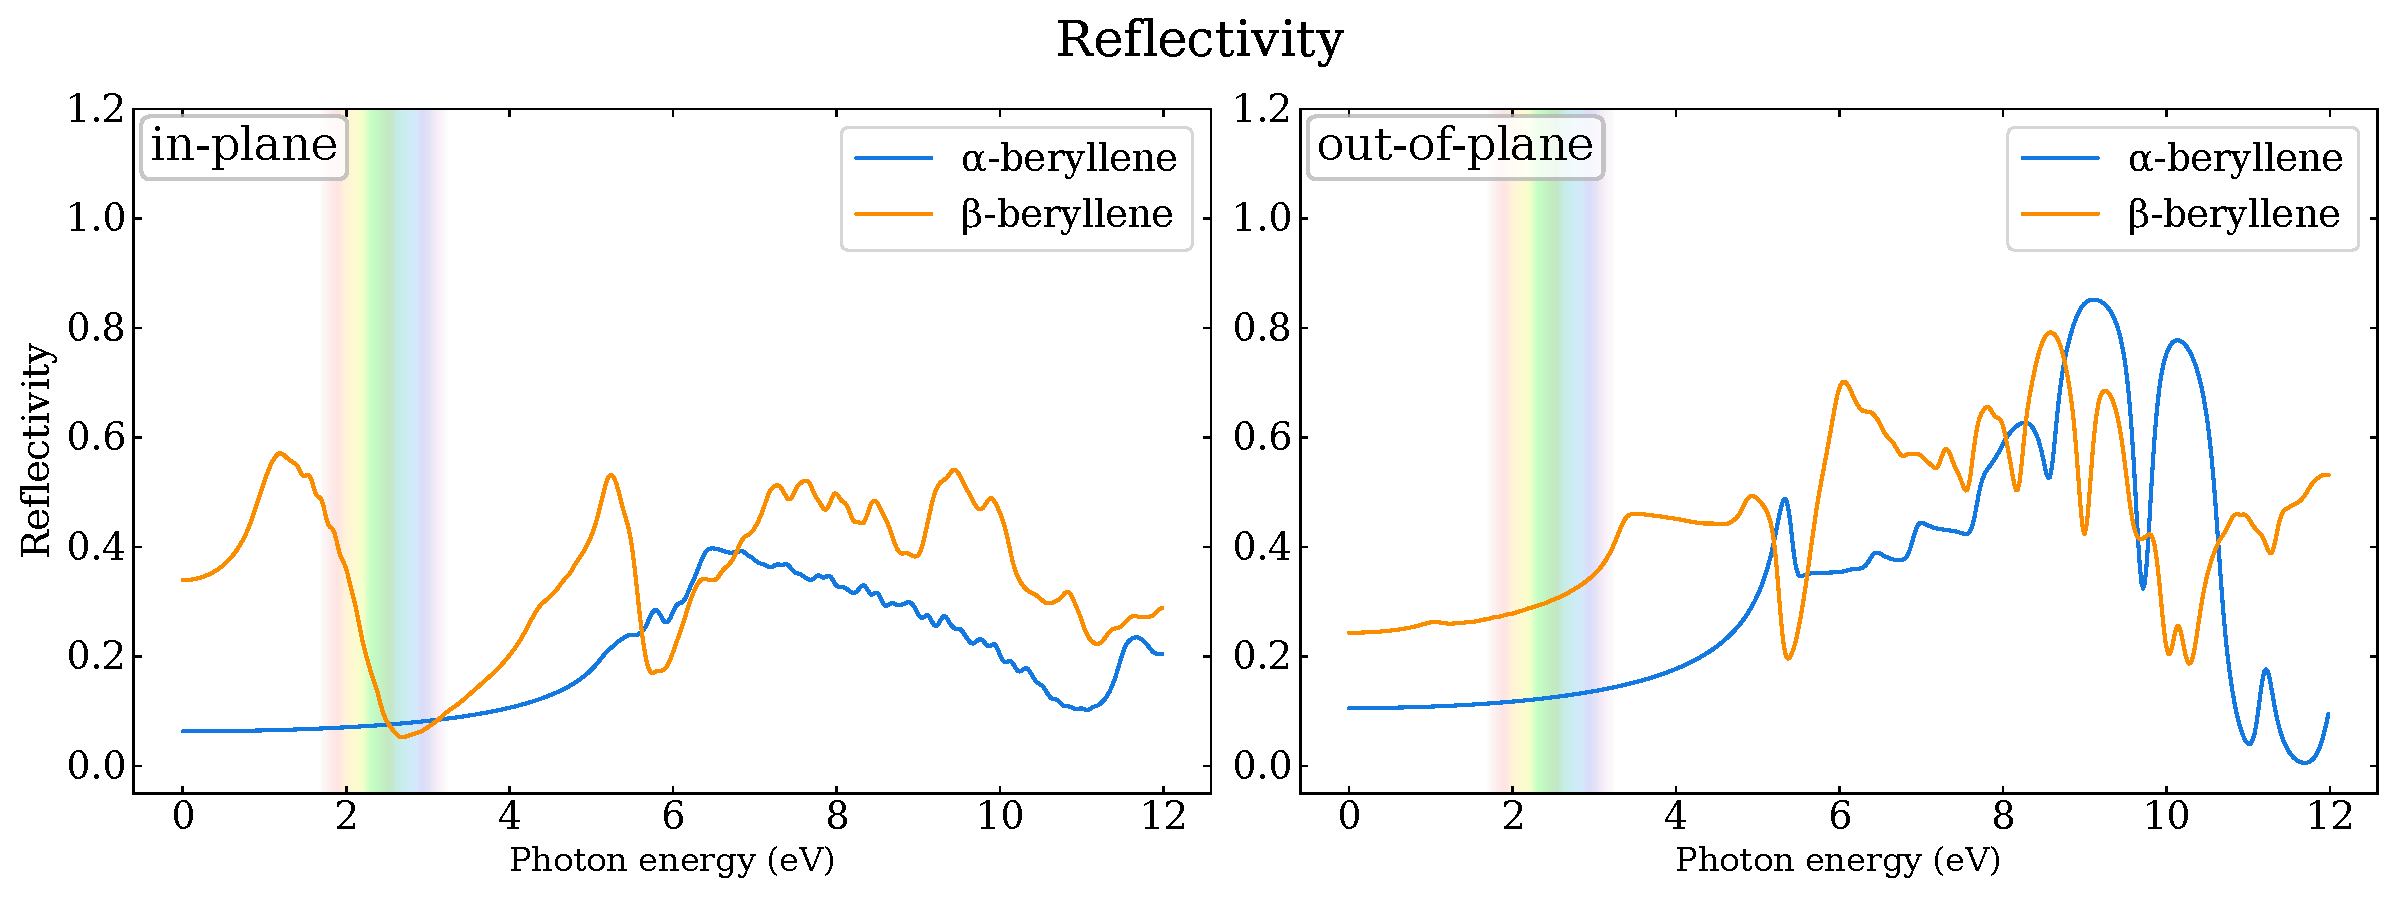
\includegraphics[width=0.80\linewidth]{figures_proj3/optics_alpha-beta_reflectivity_thesis.pdf}
\caption{Reflectivity for the in-plane and out-of-plane directions as a function of photon energy for $\alpha$-beryllene and $\beta$-beryllene.
The in-plane and out-of-plane curves correspond to the $xx$ and $zz$ components, respectively.}
\label{fig:proj3_reflectivity_alpha_beta}
\end{figure}

\begin{figure}[!htbp]
\centering
    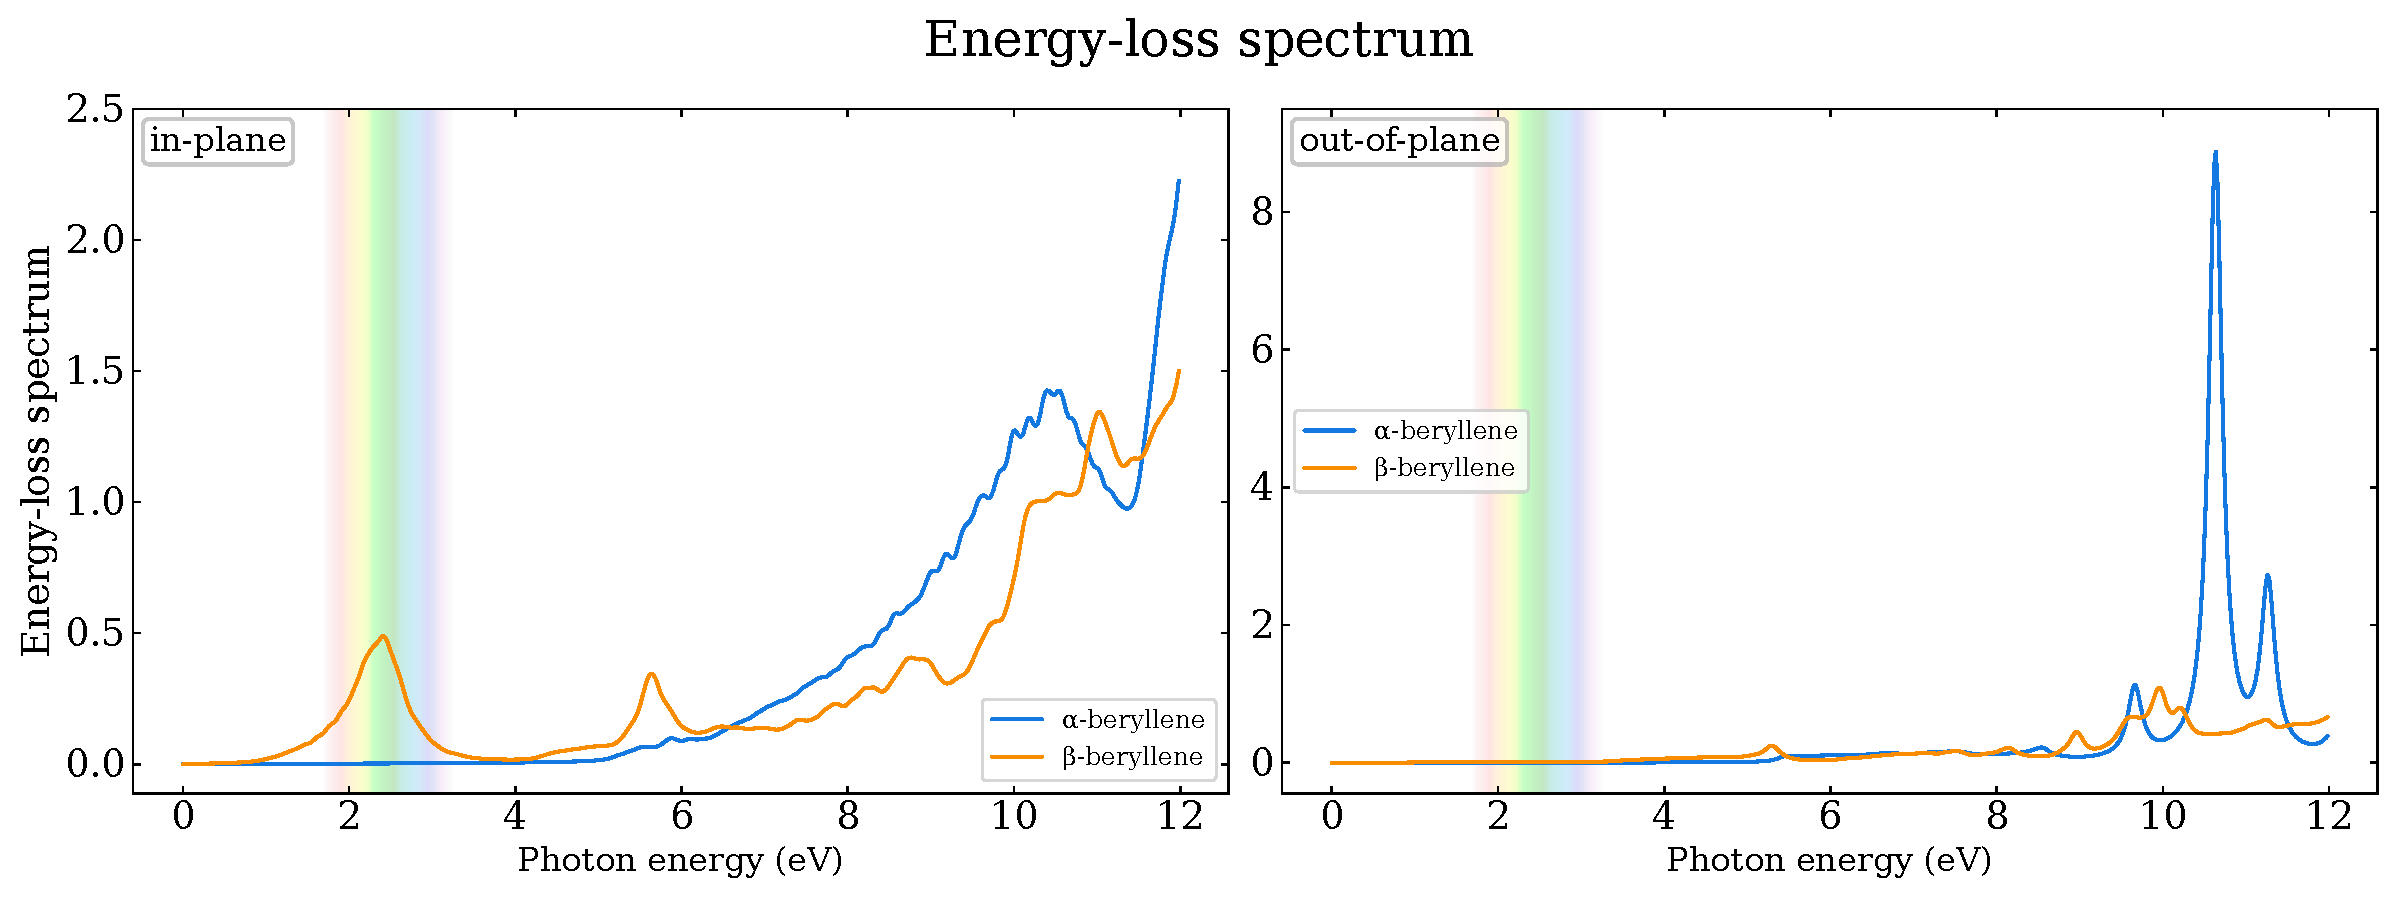
\includegraphics[width=0.80\linewidth]{figures_proj3/optics_alpha-beta_energy-loss_thesis.pdf}
\caption{Energy-loss spectrum for the in-plane and out-of-plane directions as a function of photon energy for $\alpha$-beryllene and $\beta$-beryllene.
The in-plane and out-of-plane curves correspond to the $xx$ and $zz$ components, respectively.}
\label{fig:proj3_energy_loss_alpha_beta}
\end{figure}

\begin{figure}[!htbp]
\centering
    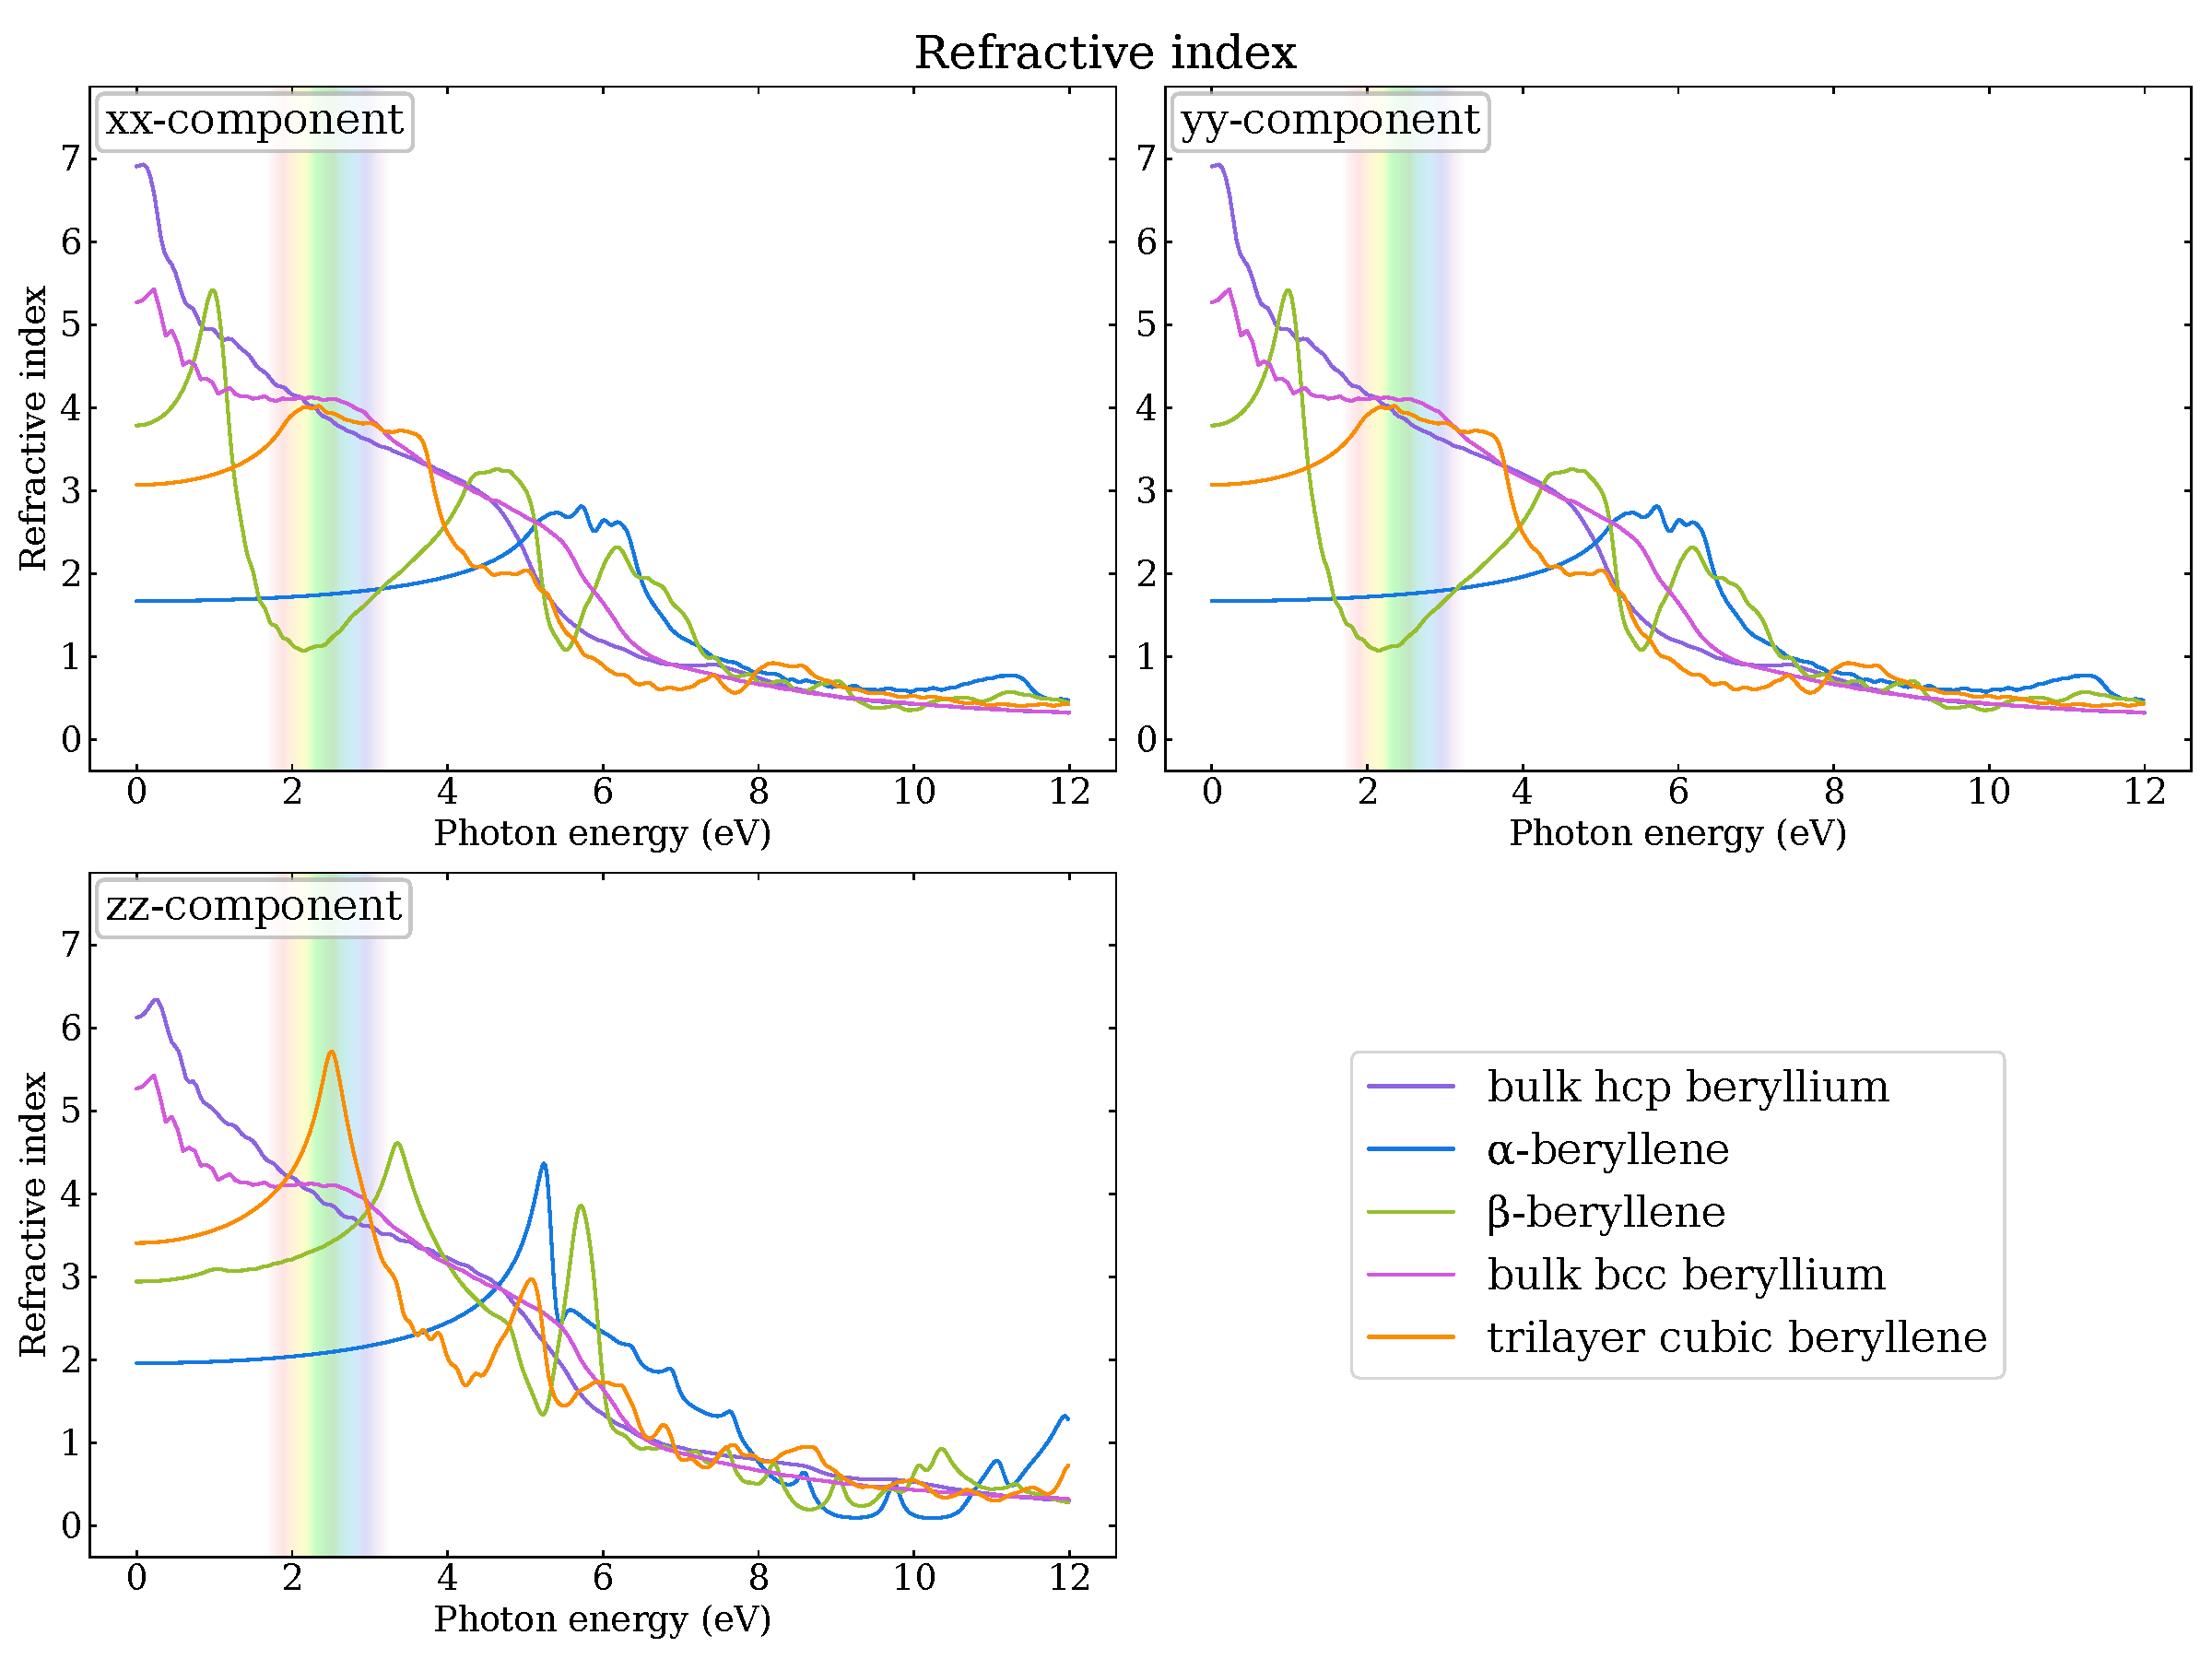
\includegraphics[width=0.80\linewidth]{figures_proj3/optics_pristine_refractive_thesis.pdf}
\caption{Refractive index for bulk hcp beryllium, $\alpha$-beryllene, $\beta$-beryllene,
bulk bcc beryllium, and trilayer cubic beryllene.
The spectra are shown for the $xx$,
$yy$,
and $zz$ components as functions of photon energy.}
\label{fig:proj3_optical_clean}
\end{figure}

\begin{figure}[!htbp]
\centering
    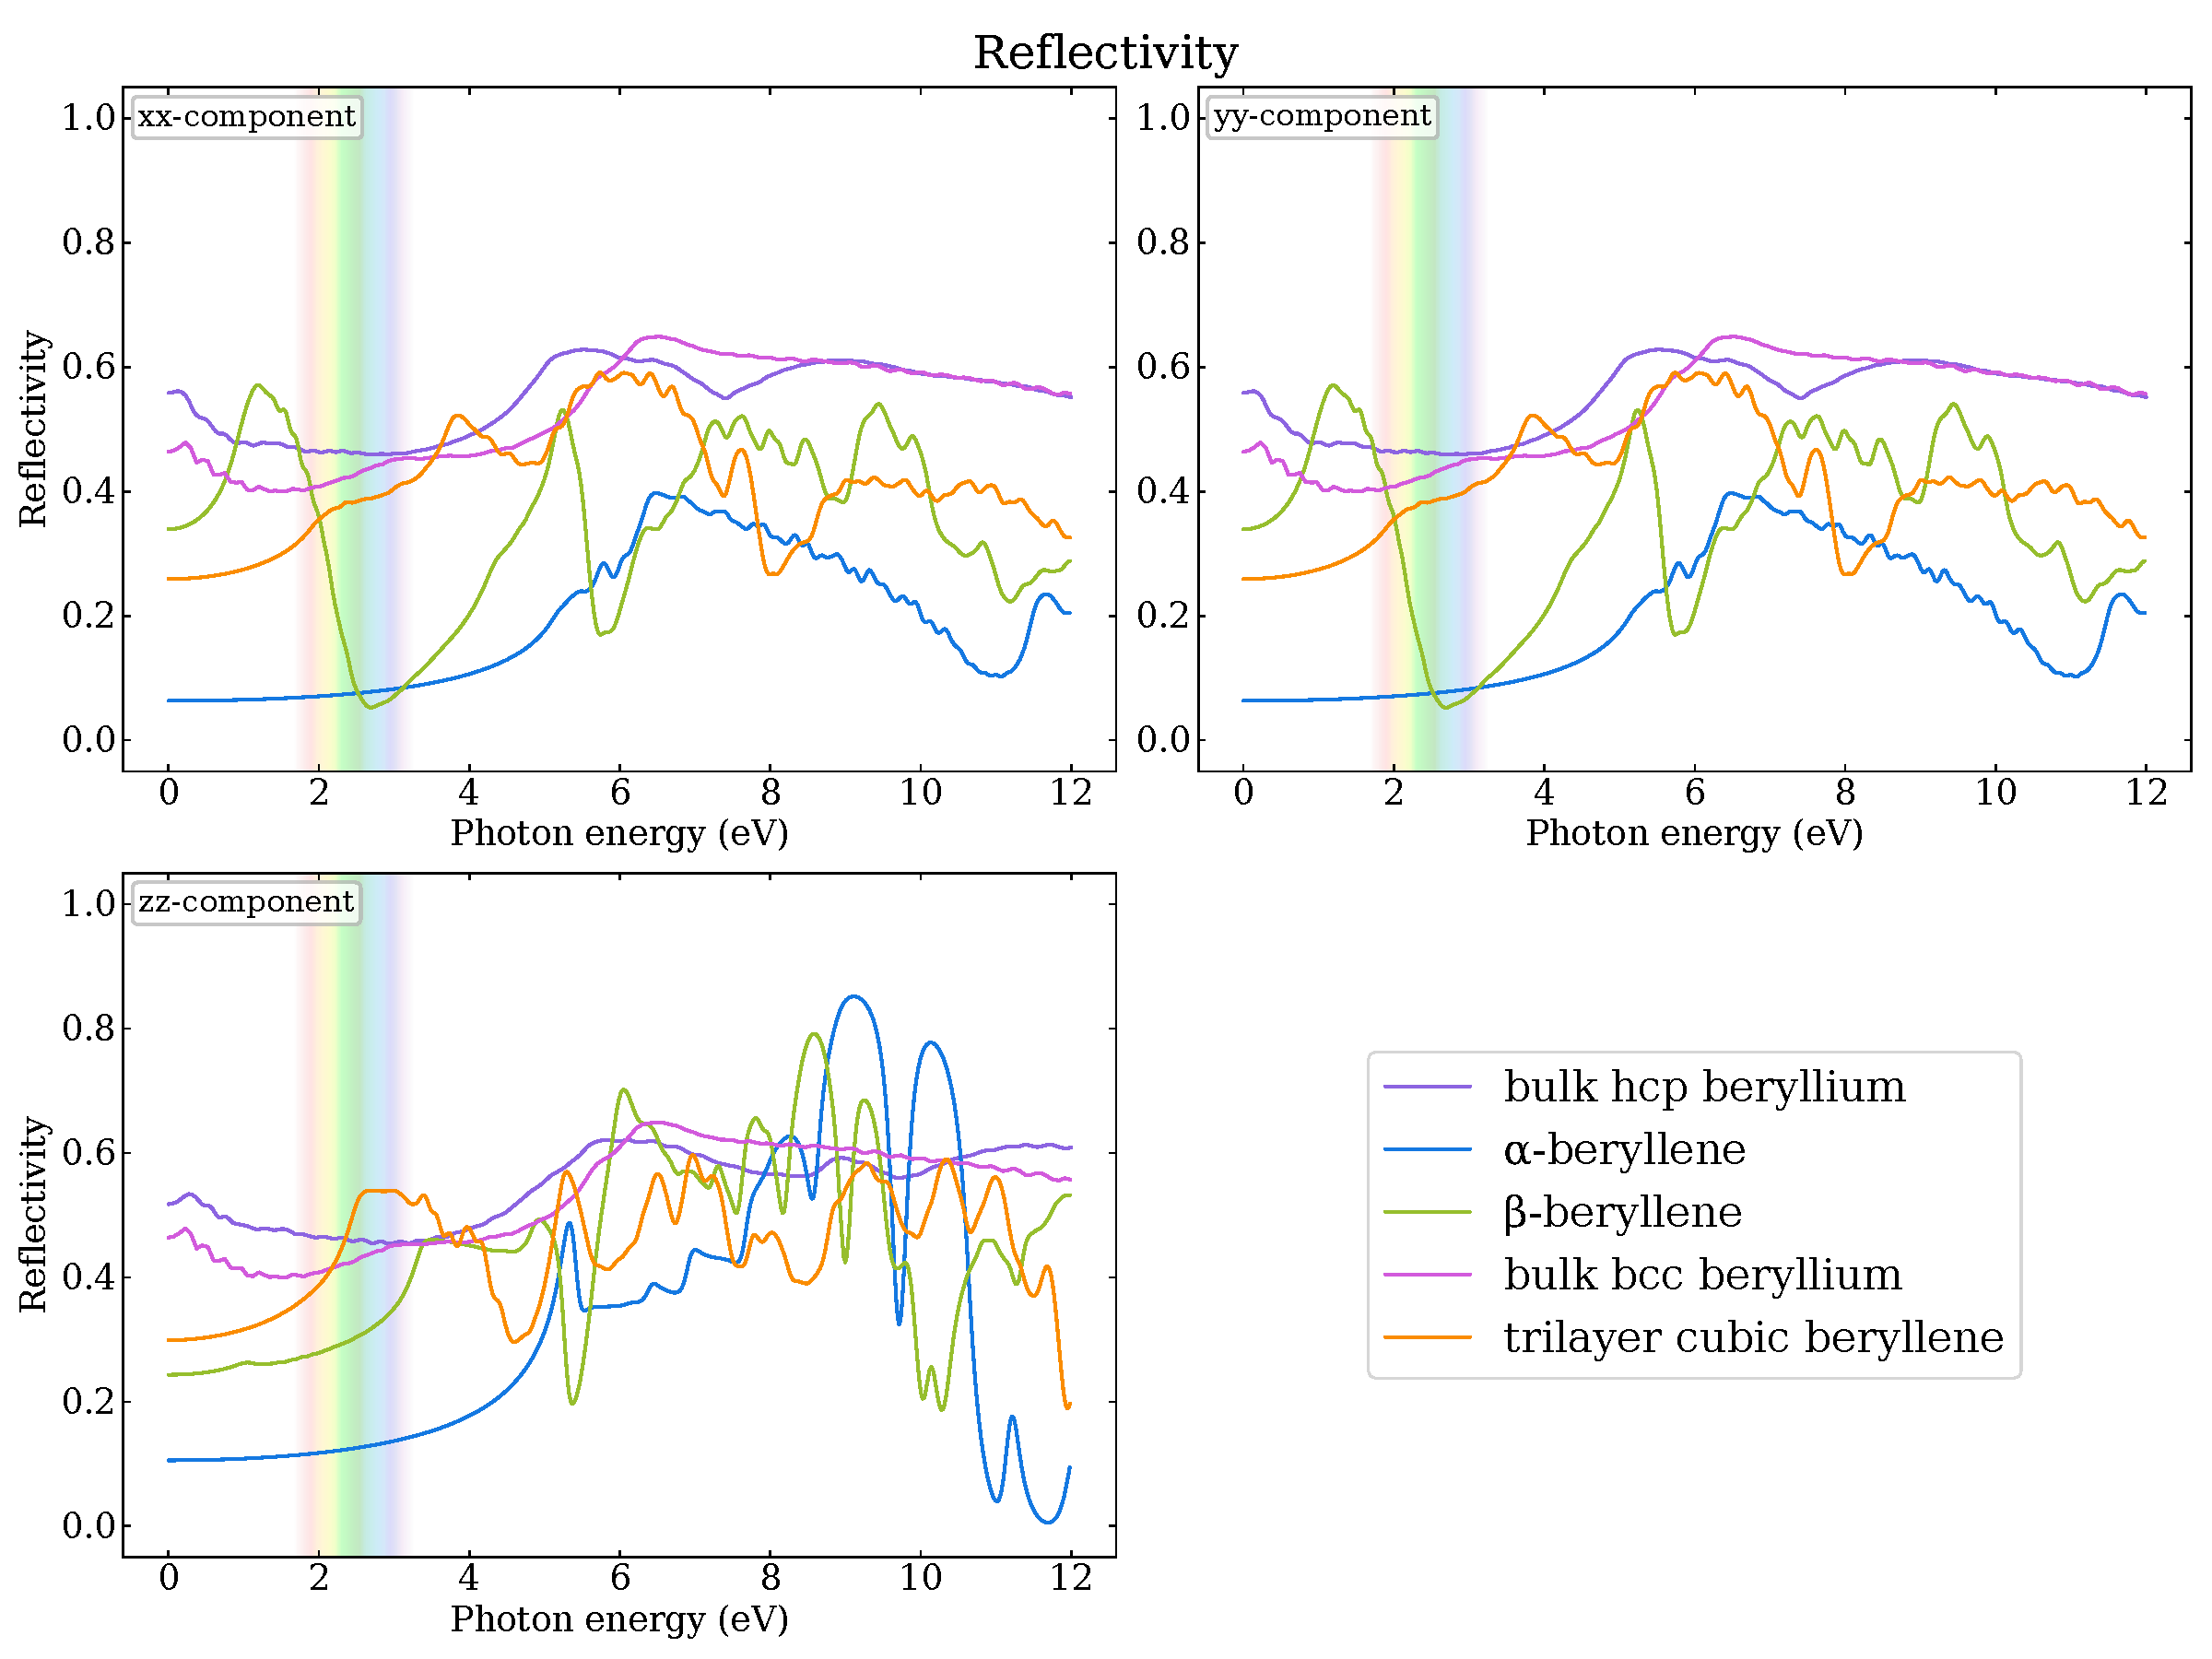
\includegraphics[width=0.80\linewidth]{figures_proj3/optics_pristine_reflectivity_thesis.pdf}
\caption{Reflectivity for bulk hcp beryllium, $\alpha$-beryllene, $\beta$-beryllene,
bulk bcc beryllium, and trilayer cubic beryllene.
The spectra are shown for the $xx$, $yy$,
and $zz$ components as functions of photon energy.}
\label{fig:proj3_optical_clean_reflectivity}
\end{figure}

\begin{figure}[!htbp]
\centering
    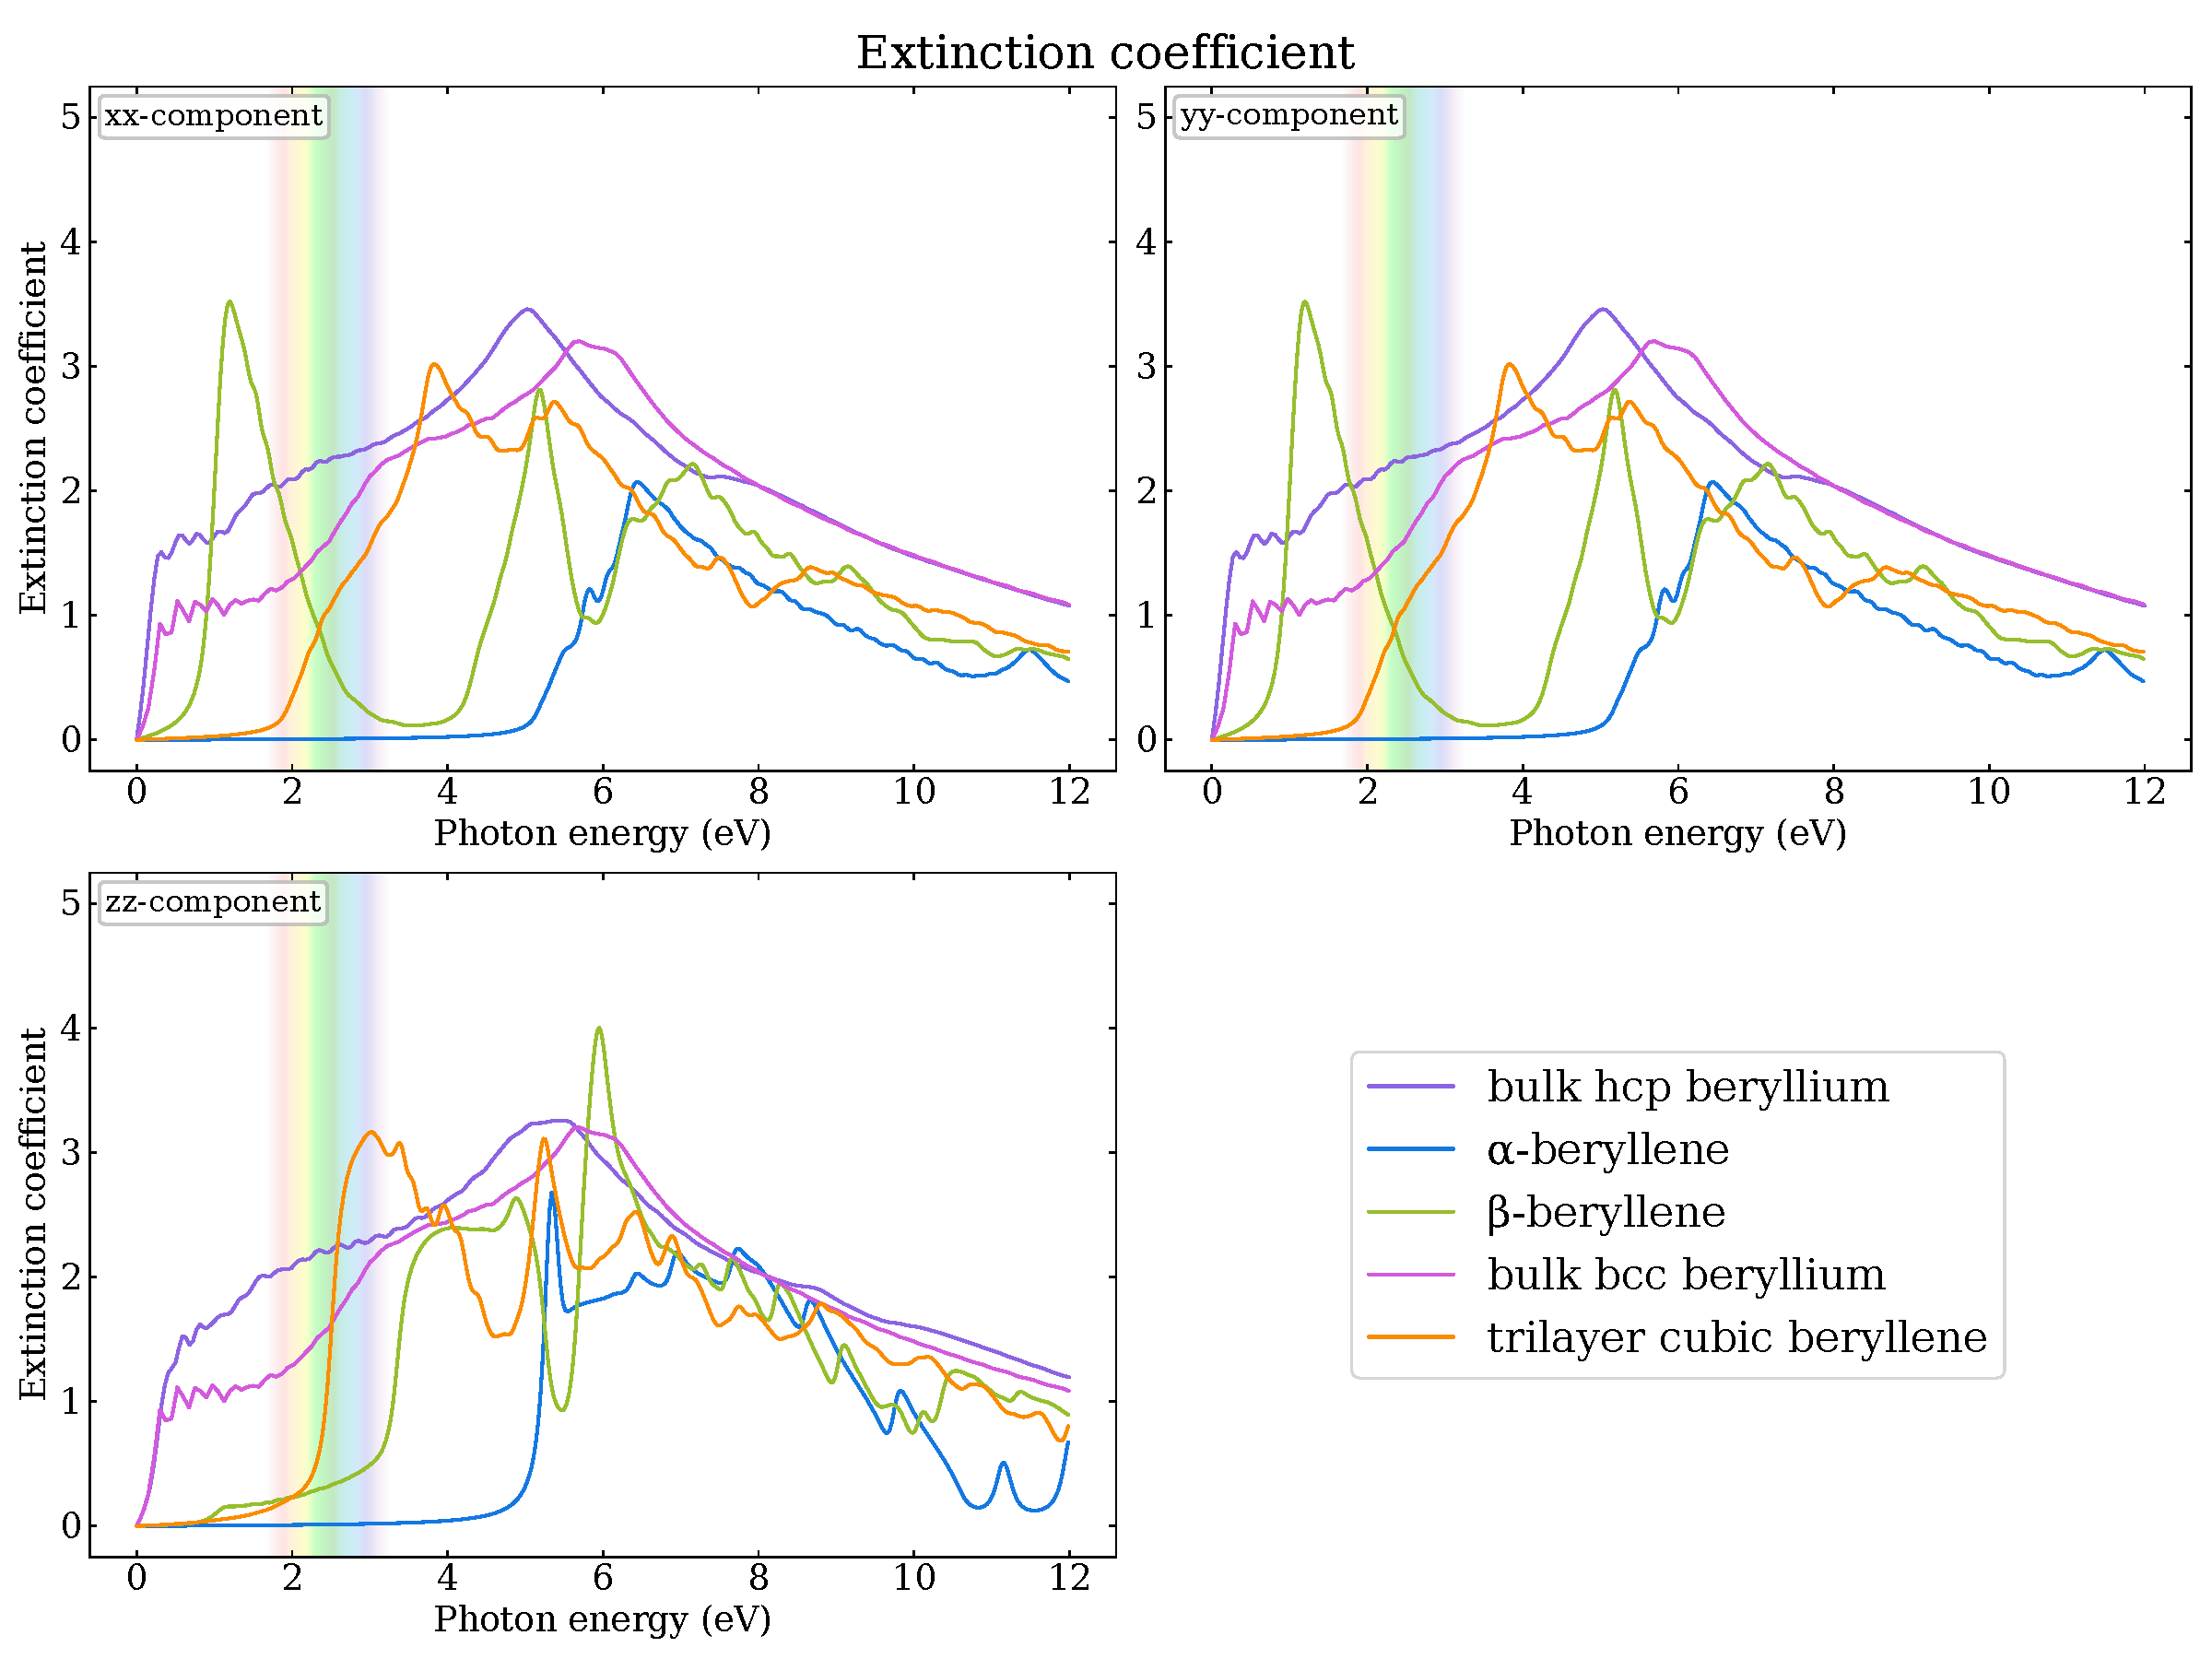
\includegraphics[width=0.80\linewidth]{figures_proj3/optics_pristine_extinction_thesis.pdf}
\caption{Extinction coefficient for bulk hcp beryllium, $\alpha$-beryllene, $\beta$-beryllene,
bulk bcc beryllium, and trilayer cubic beryllene.
The spectra are shown for the $xx$, $yy$,
and $zz$ components as functions of photon energy.}
\label{fig:proj3_optical_clean_extinction}
\end{figure}

\begin{figure}[!htbp]
\centering
    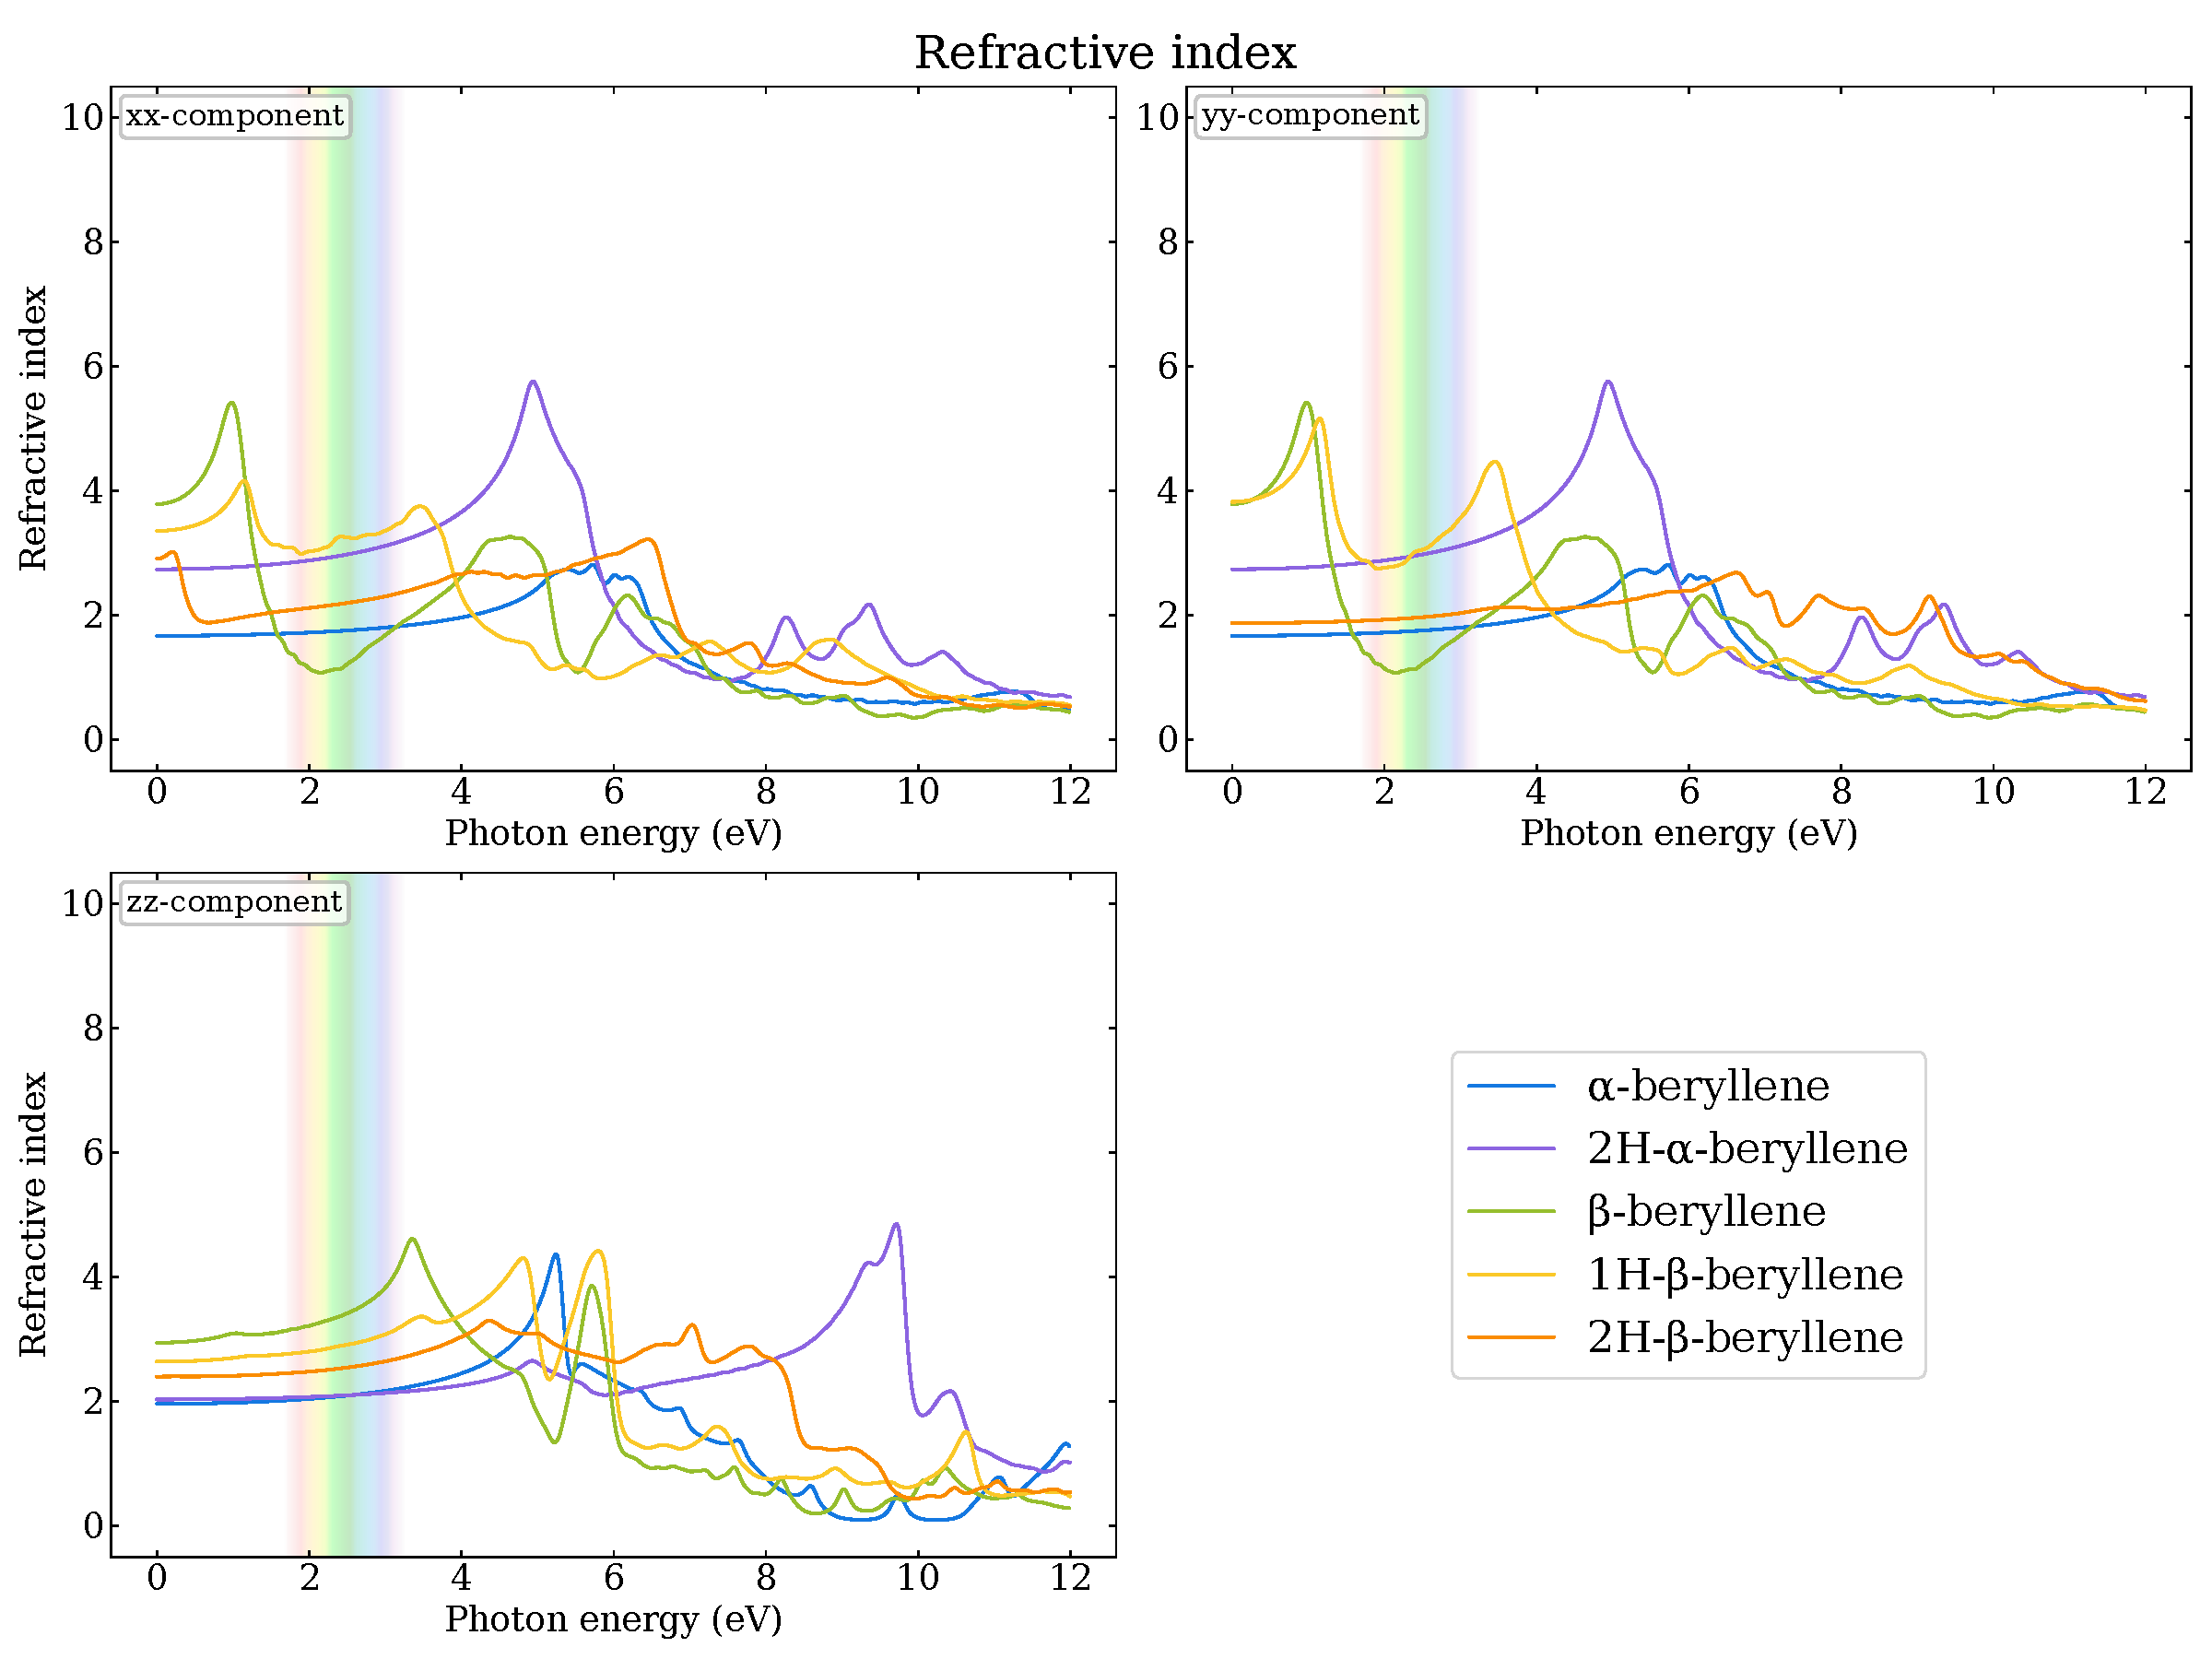
\includegraphics[width=0.80\linewidth]{figures_proj3/optics_hydrogenated_refractive_thesis.pdf}
\caption{Refractive index for pristine and hydrogen-functionalized $\alpha$-beryllene and $\beta$-beryllene structures.
The spectra are shown for the $xx$, $yy$,
and $zz$ components as functions of photon energy.}
\label{fig:proj3_optical_hydrogenated}
\end{figure}

\begin{figure}[!htbp]
\centering
    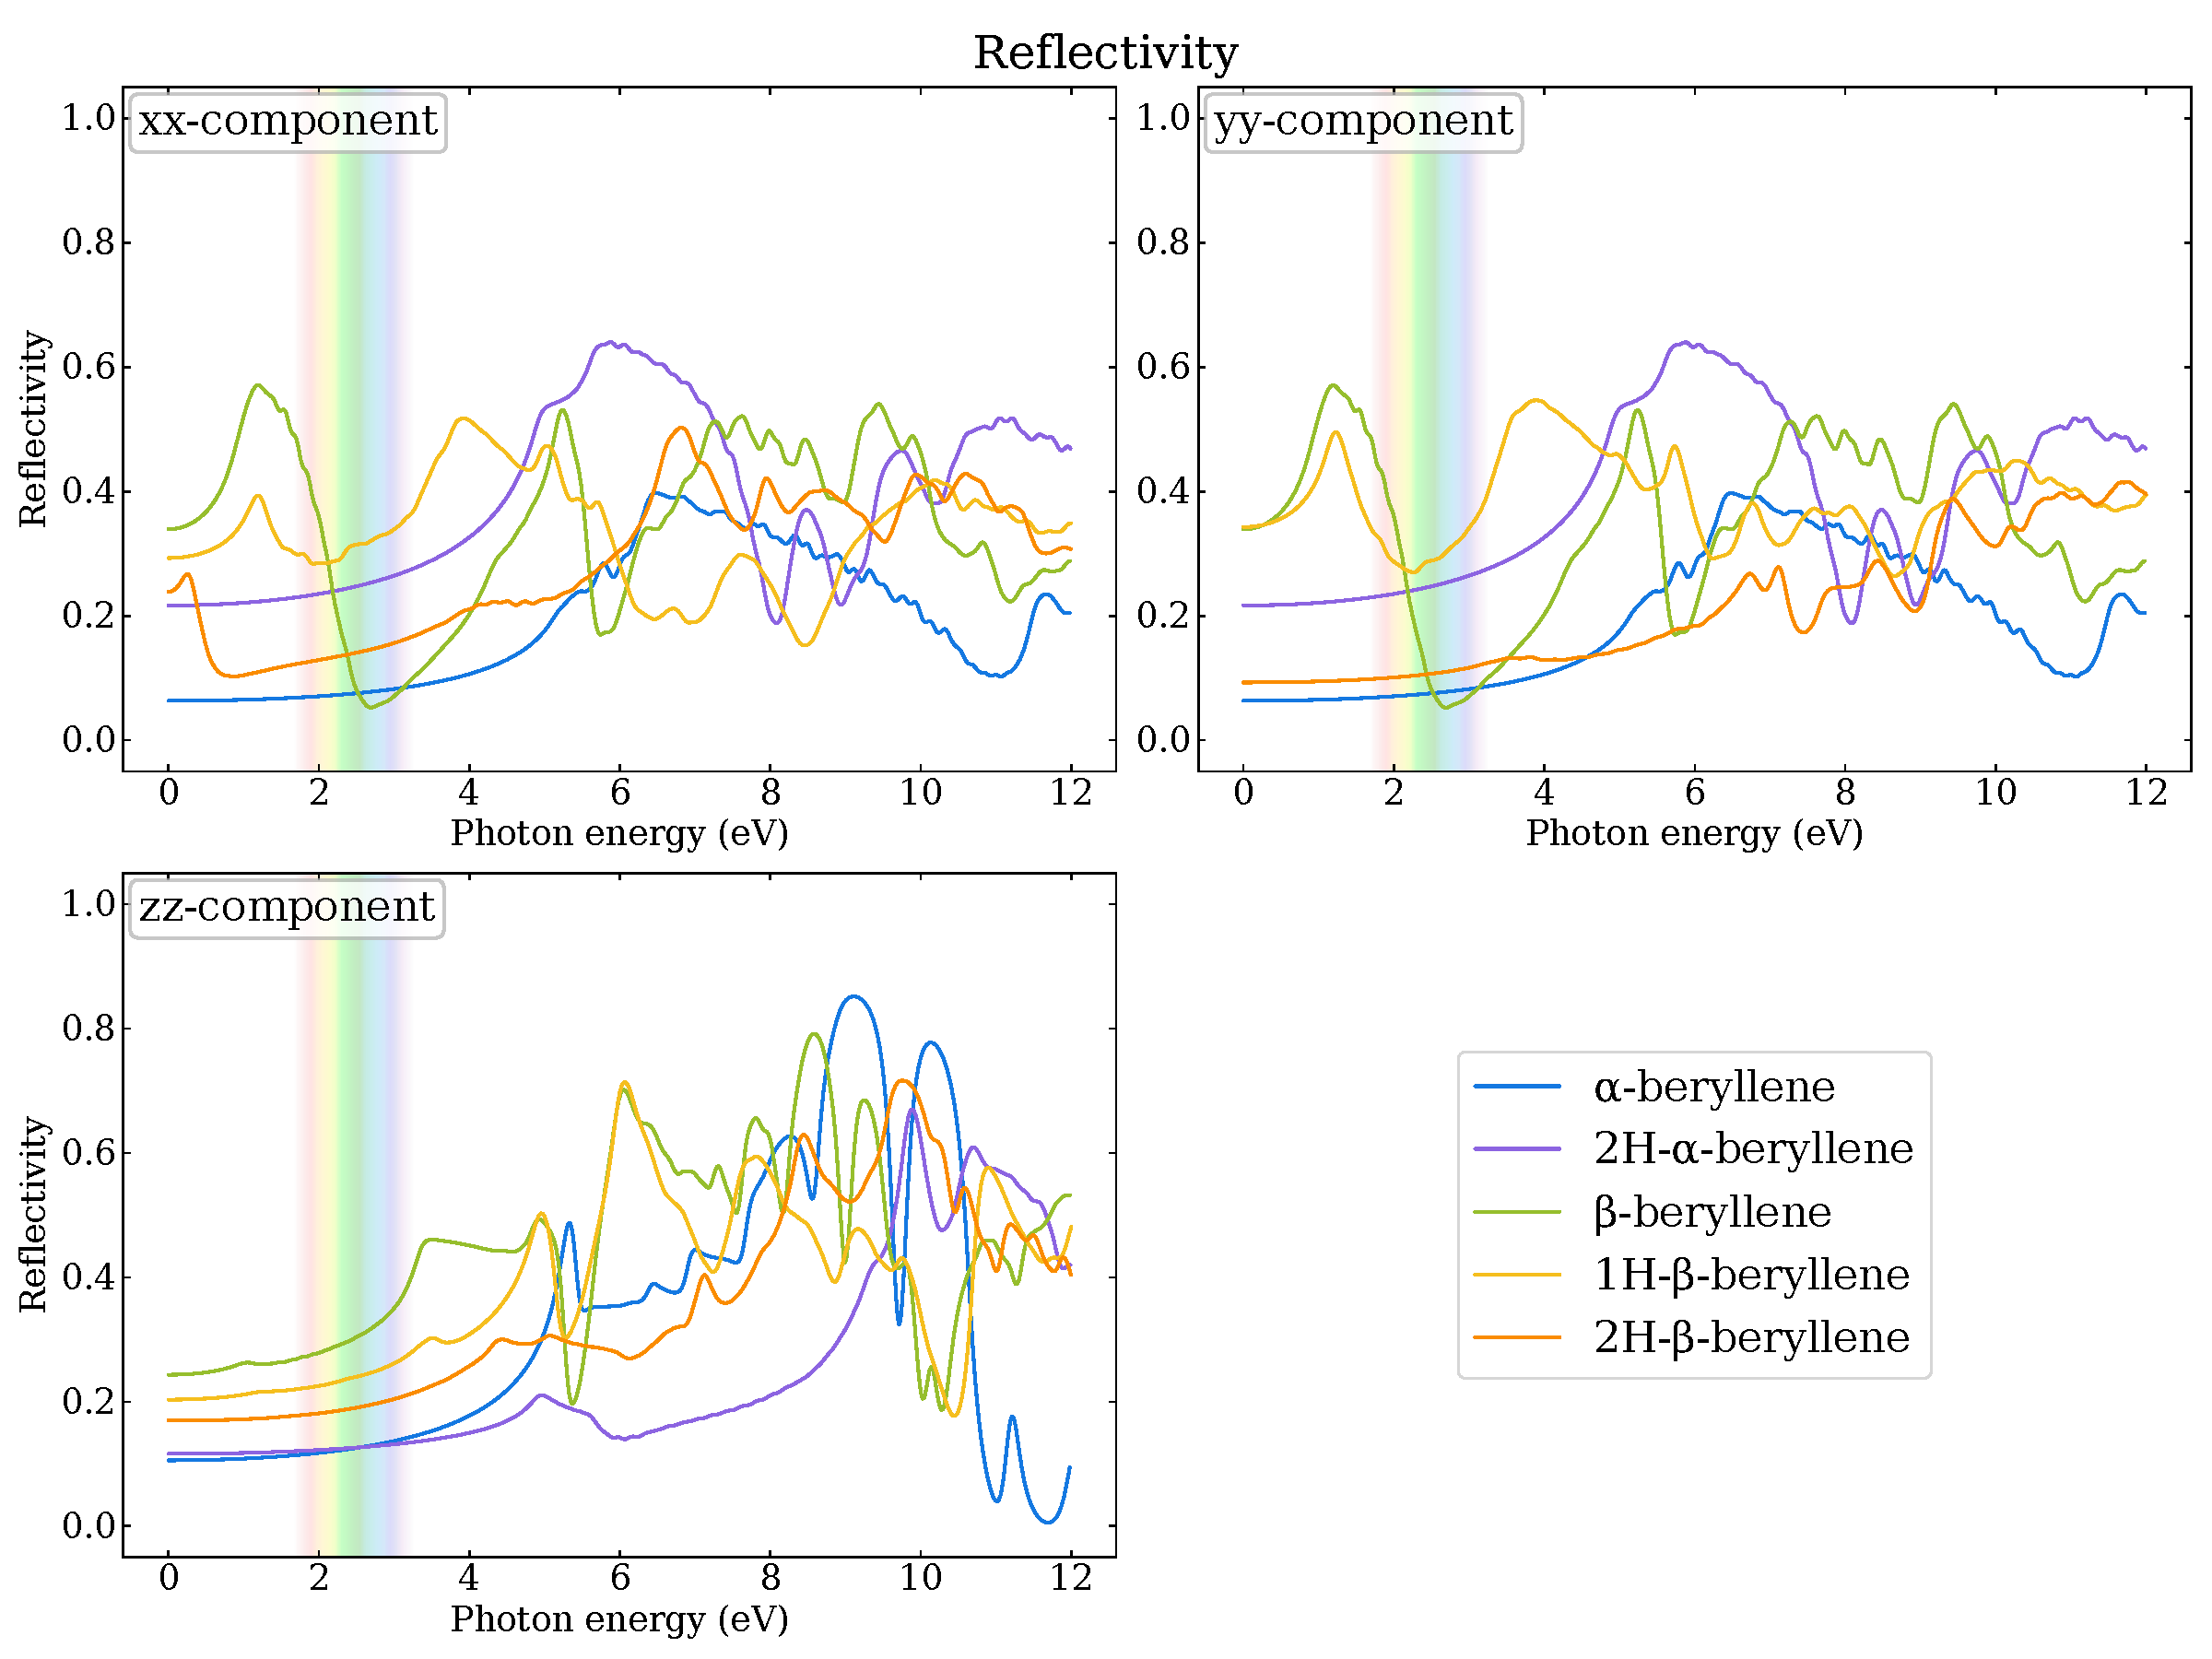
\includegraphics[width=0.80\linewidth]{figures_proj3/optics_hydrogenated_reflectivity_thesis.pdf}
\caption{Reflectivity for pristine and hydrogen-functionalized $\alpha$-beryllene and $\beta$-beryllene structures.
The spectra are shown for the $xx$, $yy$,
and $zz$ components as functions of photon energy.}
\label{fig:proj3_optical_hydrogenated_reflectivity}
\end{figure}

\begin{figure}[!htbp]
\centering
    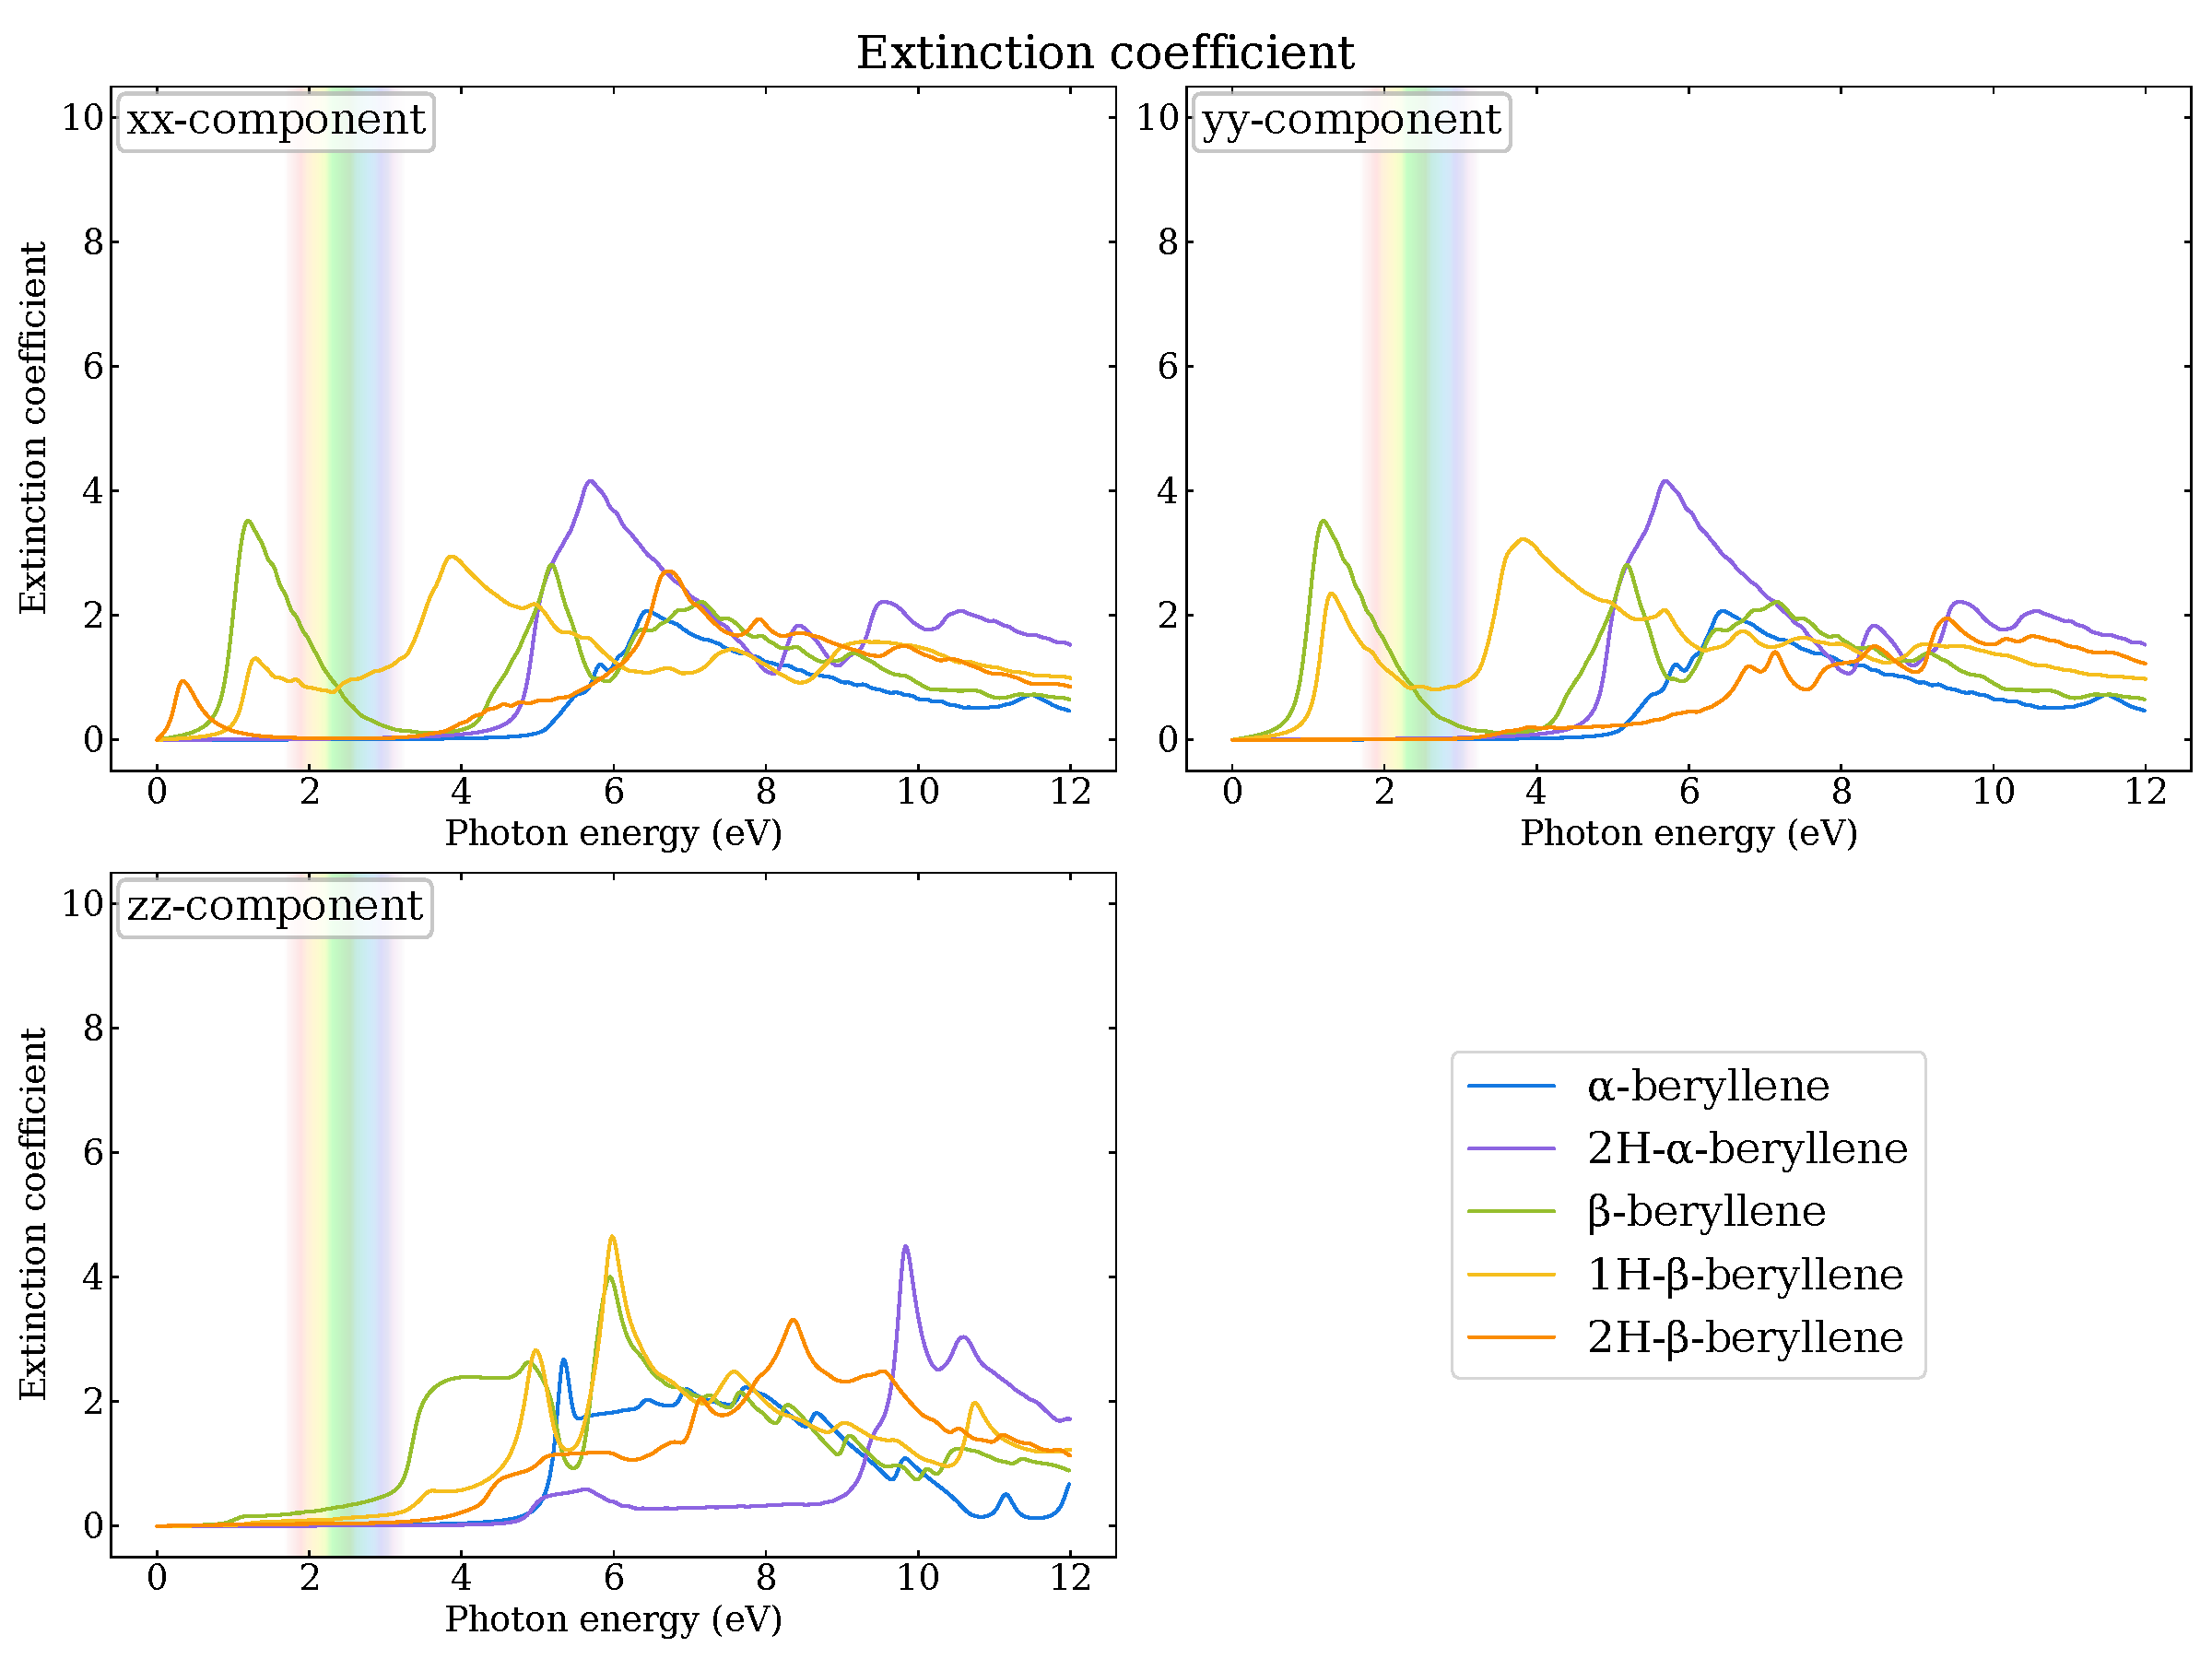
\includegraphics[width=0.80\linewidth]{figures_proj3/optics_hydrogenated_extinction_thesis.pdf}
\caption[Extinction coefficient for pristine and hydrogen-functionalized $\alpha$-beryllene and $\beta$-beryllene structures.
The spectra are shown for the $xx$, $yy$,
and $zz$ components as functions of photon energy.]{Extinction coefficient for pristine and\\
hydrogen-functionalized $\alpha$-beryllene and $\beta$-beryllene structures.
The spectra are shown for the $xx$, $yy$,
and $zz$ components as functions of photon energy.}
\label{fig:proj3_optical_hydrogenated_extinction}
\end{figure}
